%!TEX root = ../thesis.tex
%*******************************************************************************
%****************************** Third Chapter **********************************
%*******************************************************************************
\chapter{Germline and somatic mutational processes across the Tree of Life}

% **************************** Define Graphics Path **************************
\ifpdf
    \graphicspath{{Chapter3/Figs/Raster/}{Chapter3/Figs/PDF/}{Chapter3/Figs/}}
\else
    \graphicspath{{Chapter3/Figs/Vector/}{Chapter3/Figs/}}
\fi

\textit{Both in space and time, we seem to be brought somewhat near to that great fact—the mystery of mysteries—the first appearance of new beings on this earth}
\begin{flushright} [Charles Darwin] \cite{Darwin1859} \end{flushright}

\section{Introduction}

All forms of life are believed to share a common ancestor, from which their genomes are derived. The Tree of Life elegantly symbolises how various species have spawned from a single ancestor and how they are interconnected, despite their apparent physical differences. Each terminal leaf on the Tree of Life represents a species that has evolved over billions of years through the process of natural selection.

In a population, individuals exhibit a range of phenotypic diversity, and those with a selective advantage have a better chance of surviving and reproducing than others in the ongoing struggle for existence.  Somatic mutational processes and meiotic recombination are the two main mechanisms that generate genetic diversity and ultimately, phenotypic diversity.  Despite their importance in generating the genetic diversity that natural selection acts upon, research on somatic mutational process and meiotic recombination across the Tree of Life has been limited to model organisms such as \textit{C. elegans} \cite{Meier2018-cj}, \textit{D. melanogaster} \cite{McKim2002-hm} and \textit{S. cerevisiae} \cite{Gerton2000-lw}. In addition, the most recent study on somatic mutation rate in mammals with different lifespans required LCM and sequencing of colonic crypts, a clonal unit of cells, to detect somatic mutation in normal tissues \cite{Cagan2022-yn}.  This approach may not be suitable where the clonal structure of tissues is unknown, and prior knowledge of the tissue anatomy is not available. 

Above all, the lack of high-quality reference genomes and challenges associated with somatic mutation detection in bulk normal tissue have been the two critical factors that prevented the study of somatic mutational process across the Tree of Life. However, recent advances in long-read sequencing technologies, \textit{de novo} assembly and scaffolding algorithms have made it possible to construct chromosome-length scaffolds with unparalleled contiguity and completeness at a fraction of the cost and time of the hierarchical shotgun sequencing method. In chapter \ref{chapter:chapter2}, I also describe a method that leverages the base accuracy of CCS reads for somatic mutation detection in bulk normal tissue. These two developments together enable the detection of somatic mutations and the identification of new mutational signatures across the Tree of Life.  


\subsection{The Darwin Tree of Life Project}

Several initiatives have recently been launched to leverage advances in assembly and scaffolding algorithms to produce high-quality assemblies for insects \cite{Childers2021-mq}, vertebrates \cite{Rhie2021-dq} and all eukaryotic forms of life \cite{Lawniczak2022-fm}.  The DToL project is one of the initiatives that aim to sequence and assemble the genomes of 70, 000 eukaryotic species in Great Britain and Ireland \cite{Darwin_Tree_of_Life_Project_Consortium2022-ma}. To date, the DToL consortium has collected, prepared, and sequenced approximately 3000 eukaryotic samples, and has assembled the reference genomes of around 600 eukaryotic species. Here, I selected 496 eukaryotic species in the DToL project with both CCS reads and reference genomes (Table \ref{tab:dtol-samples}). Afterwards, I applied himut to 501 samples to detect somatic mutations and to identify novel and conserved somatic mutational processes across the Tree of Life (Appendix \ref{chapter:all_dtol_samples}, Figure \ref{figure:experimental-design})

\begin{figure}[htbp!]
\caption{DToL somatic mutation study experimental design}
\label{figure:experimental-design}
\begin{centering}
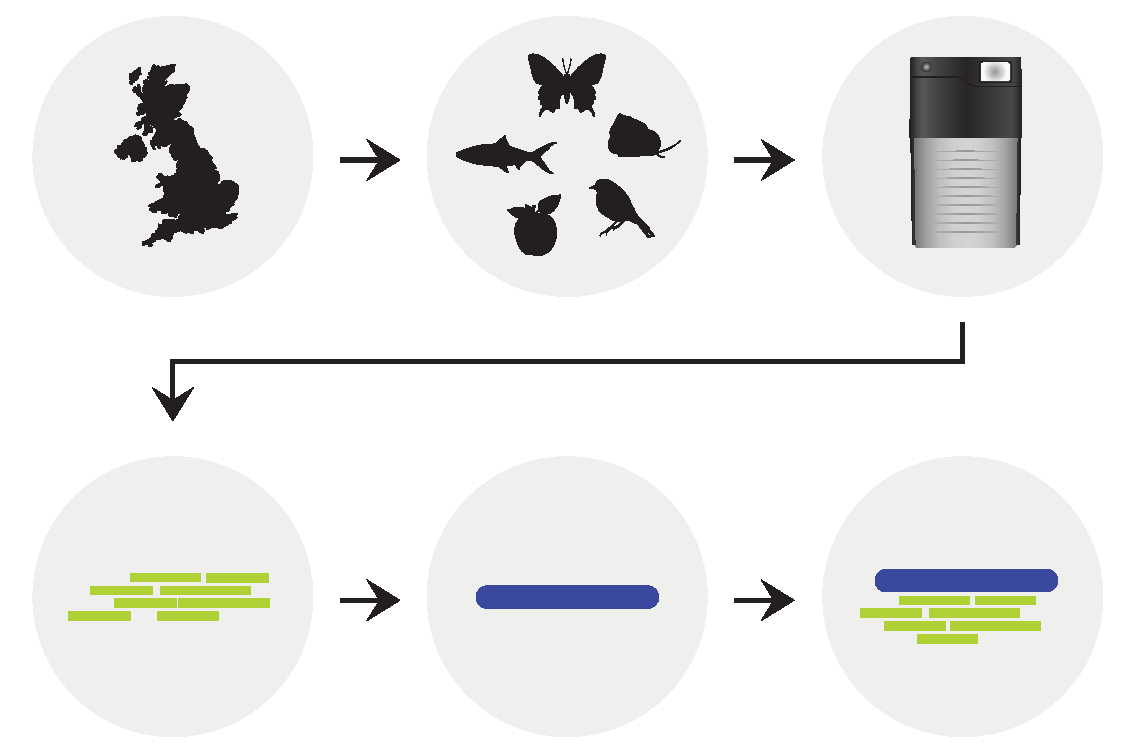
\includegraphics[width=1\textwidth]{Vector/dtol_experimental_design.pdf}
\end{centering}
\floatfoot{DToL consortium collects and sequences the sample, and generates chromosome-length scaffolds for each species. CCS reads are aligned against the reference genome and the alignment is used for both germline and somatic mutation detection.}
\end{figure}

\begin{table}[ht!]
\caption{DToL samples}
\label{tab:dtol-samples}
\begin{adjustbox}{max width=1.1\textwidth,center}
\begin{tabular}{l|l|r}
Kingdom & Taxonomic classification & Count \\ \hline
\multirow{18}{*}{Animalia}  & Annelids & 4  \\ \cline{2-3}
& Arthropods & 3  \\ \cline{2-3}
& Birds & 1  \\ \cline{2-3}
& Echinoderms & 1  \\ \cline{2-3}
& Fish & 7  \\ \cline{2-3}
& Insects (Coleoptera: Beetles)  & 30  \\ \cline{2-3}
& Insects (Diptera: Flies) & 56  \\ \cline{2-3}
& Insects (Hemiptera: True bugs) & 4  \\ \cline{2-3}
& Insects (Trichoptera: Caddisflies) & 5  \\ \cline{2-3}
& Insects (Lepidoptera: Moths and Butterflies) & 273  \\ \cline{2-3}
& Insects (Neuroptera: Net-winged insects) & 1  \\ \cline{2-3}
& Insects (Odonata: Dragonflies and Damselflies) & 2 \\ \cline{2-3}
& Insects (Plecoptera: Stoneflies) & 4  \\ \cline{2-3}
& Insects (Hymenoptera: Ants, Bees, Sawflies and Wasps) & 49  \\ \cline{2-3}
& Jellyfish & 3  \\ \cline{2-3}
& Chordates & 2  \\ \cline{2-3}
& Mammals & 5  \\ \cline{2-3}
& Molluscs & 8  \\ \hline
Fungi & Fungi & 7 \\ \hline
\multirow{2}{*}{Planta} & Dicots & 24  \\ \cline{2-3}
 & Monocots & 5 \\ \hline
Protista & Algae & 2 \\ \hline
%  & Protists & 1 \\ \hline
\end{tabular}
\floatfoot{Taxonomic classification used here follows that of the DToL consortium}
\end{adjustbox}
\end{table}

\pagebreak

\section{Materials and Methods}

\subsection{CCS library preparation, sequencing and \textit{de novo} assembly}

The DToL project initially used a combination of sequencing (CLR, CCS and linked reads) and scaffolding (e.g. Hi-C reads and BioNano genome maps) technologies to generate chromosome-length scaffolds. The DToL project currently uses HiFiAdapterFilter \cite{Sim2022-pi} to remove CCS reads with adapter sequences, either hifiasm \cite{Cheng2021-ij} or hicanu \cite{Nurk2020-gu} for \text{de novo} assembly of contigs from CCS reads, purgedups \cite{Guan2020-tl} to remove haplotype duplication, arrow \cite{Chin2016-at} for contig polishing and SALSA2 \cite{Ghurye2019-ua} to order and orient contigs into chromosome-length scaffolds with Hi-C reads. If both the parent and child were sequenced, trio-canu \cite{Koren2018-wg} was used to generate haplotype phased contigs. Afterwards, the chromosome-length scaffolds were manually curated using a Hi-C contact matrix to identify and correct misassemblies and to perform additional scaffolding where appropriate. If transcriptome data were available through either RNA or isoform sequencing, gene annotation was also performed in collaboration with the EMBL-EBI eukaryotic annotation team. The specific method and algorithm described here was subject to change with updates to the sequencing method, \textit{de novo} assembly and scaffolding algorithm. 

\subsection{\textit{Phorcus lineatus} somatic mutation rate measurement}

To calculate the somatic mutation rate of \textit{P. lineatus} (thick top shell), samples of different ages (3, 5 and 15) were collected from Plymouth, UK. Collaborators at the Marine Biological Association determined the age of the samples from growth marks on the shells of samples. As recommended, a bench-mounted vice was first used to crush the shell and to carefully separate the sample from the shell (personal communication with Robert Mrowicki at the MBA). In addition, disposable scalpels were used during the dissection to prevent cross-contamination between the samples. HMW DNA was subsequently extracted from the foot muscle using the Circulomics Nanobind Tissue Big DNA Kit (SKU 102-302-100). CCS libraries were prepared following the low-input CCS library preparation protocol and BluePippin system was used to size select CCS libraries prior to sequencing.

CCS BQ score is a function of the number of supporting subreads and the concordance between the CCS base and subread bases. The DNAP processivity and CCS read length determine the number of full-length subreads per CCS read, which in turn influences the number of Q93 CCS bases from which potential somatic mutations can be identified. To account for the differences in the number of subreads per CCS read for each ZMW, the raw subreads BAM file was parsed using a custom script to select 10 full-length subreads per ZMW. The script calculates the median subread length for each ZMW and considers subreads between 0.8 times the median subread length and 1.2 times the median subread length as full-length subreads. The processed subreads BAM file was, thereafter, provided as an input to the pbccs algorithm to re-generate CCS reads. CCS reads were subsequently processed as described below. Apart from calculating the somatic mutation rate in \textit{P. lineatus}, CCS reads produced with the default pbccs parameters are used for all other remaining analysis.

\subsection{Germline and somatic mutation detection across the Tree of Life}

As detailed in section \ref{sec:himut}, CCS reads with adapter sequences were identified using HiFiAdapterFilt \cite{Sim2022-pi} and discarded. In addition, if ultra-low input CCS library preparation protocol was used for CCS generation and if this was documented, CCS reads were also excluded from downstream sequence analysis (this information, however, was not always available). Thereafter, CCS reads were aligned to the assembled reference genomes using minimap2 \cite{Li2018-am} and primary alignments were selected, sorted and merged into a single BAM file using samtools \cite{Li2011-ag}. Germline mutations were called using deepvariant \cite{Poplin2018-ub}. Somatic mutations were detected, and mutation burden for each sample was calculated using himut. 

As CCS reads and reference genomes are derived from the same sample, homozygous alternative allele indicate assembly errors and analysis of germline mutations are restricted to heterozygous mutations for samples with a diploid genome. On the other hand, if a sample has a haploid genome, heterozygous mutations are not expected from the sample. In the order Hymenoptera, male individuals develop from an unfertilised egg and have a haploid genome. 

The detection of somatic mutations across the tree of life required some minor modifications to reflect differences in the experimental design and sample heterozygosity. When somatic mutations were called from DToL eukaryotic species, a VCF file containing germline mutations was supplied to himut to calculate heterozygosity ($\theta$) and the genotype prior $P(G)$. In addition, because a single sample was sequenced per species and as population-scale sequencing studies have not been performed for these species, a PoN VCF file could not be generated and a VCF file with common SNPs were not available to distinguish false positive substitutions arising from systematic errors and gDNA contamination, respectively. However, given that CCS library and the reference genome originate from the same sample, false positive substitutions arising from alignment errors should be minimised and CCS reads resulting from gDNA contamination should be excluded from the analysis based on their sequence identity or their haplotype.

\subsection{Mutational signature extraction and analysis}


As described in section \ref{sec:mutational_signature_analysis}, there are 6 substitution types (C>A, C>G, C>T, T>A, T>C, T>G) in the pyrimidine context and 16 trinucleotide sequence contexts for each substitution class, creating the canonical SBS96 classification system. Since the ancestral allele is known for somatic mutations, the SBS96 classification system is often used to categorise somatic substitutions. In contrast, because the ancestral allele is unknown for germline mutations, the SBS52 classification system is used for germline substitution classification. 

Here, I describe the SBS52 classification system and how the SBS96 classification system is transformed into the SBS52 classification system (Table \ref{tab:SBS96-to-SBS52}). The need for the SBS52 classification system arises from the fact that certain germline substitutions are indistinguishable from one another because the reference base cannot be assumed to be the ancestral allele; Because the reference genome is sequenced and assembled from a randomly sampled individual, another individual could with a different germline mutation could have easily been used for reference genome construction. For instance, a C>A substitution in the AAA trinucleotide sequence context on the forward strand cannot be distinguished from a T>G substitution in the TTT trinucleotide sequence context on the reverse strand. Similarly, C>T substitutions cannot be differentiated from T>C substitutions. Moreover, a C>G (T>A) substitution occurring at a specific trinucleotide is interchangeable with C>G (T>A) substitution at a different trinucleotide

After categorising germline and somatic substitutions based on the SBS52 and SBS96 classification system, SBS52 and SBS96 counts were processed as described below for \textit{de novo} mutational signature extraction using HDP \cite{hdp2018} with 10 independent chains with a burn-in of 20,000. Following mutational signature extraction, cosine similarity between somatic and germline mutation signatures were measured to identify mutational processes shared between the germline and the soma. To enable their comparison, somatic mutation signatures were transformed from the SBS96 classification system to the SBS52 classification system and cosine similarity between soma and germline-derived mutational signatures were measured. Afterwards, germline and soma mutational signatures with the highest cosine similarity were determined to be the same mutational signature. 

Here, I focused on mutational signatures that were both present in the germline and the soma, and somatic mutational signatures that exhibited transcriptional strand-bias. To determine whether the identified mutational signatures are conserved across different eukaryotic lineages, the proportion of samples with the mutational signature were calculated for each taxonomic classification. A sample was ascertained to have somatic mutational process that generates the mutational signature, if the mutational signature contributes to more than 10\% of the mutations in the sample.

\newpage

\begingroup
\setlength{\LTleft}{-20cm plus -1fill} %% centering
\setlength{\LTright}{\LTleft}
\begin{longtable}{c|c|c}
\label{tab:SBS96-to-SBS52} \\ \smallskip
SBS52 & \makecell{forward strand \\ (reference centred)} & \makecell{reverse strand \\ (read centred)}  \\ \hline
\ttfamily A[C>A]A & \ttfamily ACA>AAA = A[C>A]A & \ttfamily TTT>TGT = T[T>G]T \\ \hline
\ttfamily A[C>A]C & \ttfamily ACC>AAC = A[C>A]C & \ttfamily GTT>GGT = G[T>G]T \\ \hline
\ttfamily A[C>A]G & \ttfamily ACG>AAG = A[C>A]G & \ttfamily CTT>CGT = C[T>G]T \\ \hline
\ttfamily A[C>A]T & \ttfamily ACT>AAT = A[C>A]T & \ttfamily ATT>AGT = A[T>G]T \\ \hline
\ttfamily C[C>A]A & \ttfamily CCA>CAA = C[C>A]A & \ttfamily TTG>TGG = T[T>G]G \\ \hline
\ttfamily C[C>A]C & \ttfamily CCC>CAC = C[C>A]C & \ttfamily GTG>GGG = G[T>G]G \\ \hline
\ttfamily C[C>A]G & \ttfamily CCG>CAG = C[C>A]G & \ttfamily CTG>CGG = C[T>G]G \\ \hline
\ttfamily C[C>A]T & \ttfamily CCT>CAT = C[C>A]T & \ttfamily ATG>AGG = A[T>G]G \\ \hline
\ttfamily G[C>A]A & \ttfamily GCA>GAA = G[C>A]A & \ttfamily TTC>TGC = T[T>G]C \\ \hline
\ttfamily G[C>A]C & \ttfamily GCC>GAC = G[C>A]C & \ttfamily GTC>GGC = G[T>G]C \\ \hline
\ttfamily G[C>A]G & \ttfamily GCG>GAG = G[C>A]G & \ttfamily CTC>CGC = C[T>G]C \\ \hline
\ttfamily G[C>A]T & \ttfamily GCT>GAT = G[C>A]T & \ttfamily ATC>AGC = A[T>G]C \\ \hline
\ttfamily T[C>A]A & \ttfamily TCA>TAA = T[C>A]A & \ttfamily TTA>TGA = T[T>G]A \\ \hline
\ttfamily T[C>A]C & \ttfamily TCC>TAC = T[C>A]C & \ttfamily GTA>GGA = G[T>G]A \\ \hline
\ttfamily T[C>A]G & \ttfamily TCG>TAG = T[C>A]G & \ttfamily CTA>CGA = C[T>G]A \\ \hline
\ttfamily T[C>A]T & \ttfamily TCT>TAT = T[C>A]T & \ttfamily ATA>AGA = A[T>G]A \\ \hline
\ttfamily A[C>T]A & \ttfamily ACA>ATA = A[C>T]A & \ttfamily TAT>TGT = A[T>C]A \\ \hline
\ttfamily A[C>T]C & \ttfamily ACC>ATC = A[C>T]C & \ttfamily GAT>GGT = A[T>C]C \\ \hline
\ttfamily A[C>T]G & \ttfamily ACG>ATG = A[C>T]G & \ttfamily CAT>CGT = A[T>C]G \\ \hline
\ttfamily A[C>T]T & \ttfamily ACT>ATT = A[C>T]T & \ttfamily AAT>AGT = A[T>C]T \\ \hline
\ttfamily C[C>T]A & \ttfamily CCA>CTA = C[C>T]A & \ttfamily TAG>TGG = C[T>C]A \\ \hline
\ttfamily C[C>T]C & \ttfamily CCC>CTC = C[C>T]C & \ttfamily GAG>GGG = C[T>C]C \\ \hline
\ttfamily C[C>T]G & \ttfamily CCG>CTG = C[C>T]G & \ttfamily CAG>CGG = C[T>C]G \\ \hline
\ttfamily C[C>T]T & \ttfamily CCT>CTT = C[C>T]T & \ttfamily AAG>AGG = C[T>C]T \\ \hline
\ttfamily G[C>T]A & \ttfamily GCA>GTA = G[C>T]A & \ttfamily TAC>TGC = G[T>C]A \\ \hline
\ttfamily G[C>T]C & \ttfamily GCC>GTC = G[C>T]C & \ttfamily GAC>GGC = G[T>C]C \\ \hline
\ttfamily G[C>T]G & \ttfamily GCG>GTG = G[C>T]G & \ttfamily CAC>CGC = G[T>C]G \\ \hline
\ttfamily G[C>T]T & \ttfamily GCT>GTT = G[C>T]T & \ttfamily AAC>AGC = G[T>C]T \\ \hline
\ttfamily T[C>T]A & \ttfamily TCA>TTA = T[C>T]A & \ttfamily TAA>TGA = T[T>C]A \\ \hline
\ttfamily T[C>T]C & \ttfamily TCC>TTC = T[C>T]C & \ttfamily GAA>GGA = T[T>C]C \\ \hline
\ttfamily T[C>T]G & \ttfamily TCG>TTG = T[C>T]G & \ttfamily CAA>CGA = T[T>C]G \\ \hline
\ttfamily T[C>T]T & \ttfamily TCT>TTT = T[C>T]T & \ttfamily AAA>AGA = T[T>C]T \\ \hline
\ttfamily A[C>G]A & \ttfamily ACA>AGA = A[C>G]A & \ttfamily TCT>TGT = T[C>G]T \\ \hline
\ttfamily A[C>G]C & \ttfamily ACC>AGC = A[C>G]C & \ttfamily GCT>GGT = G[C>G]T \\ \hline
\ttfamily A[C>G]G & \ttfamily ACG>AGG = A[C>G]G & \ttfamily CCT>CGT = C[C>G]T \\ \hline
\ttfamily A[C>G]T & \ttfamily ACT>AGT = A[C>G]T & \ttfamily ACT>AGT = A[C>G]T \\ \hline
\ttfamily C[C>G]A & \ttfamily CCA>CGA = C[C>G]A & \ttfamily TCG>TGG = T[C>G]G \\ \hline
\ttfamily C[C>G]C & \ttfamily CCC>CGC = C[C>G]C & \ttfamily GCG>GGG = G[C>G]G \\ \hline
\ttfamily C[C>G]G & \ttfamily CCG>CGG = C[C>G]G & \ttfamily CCG>CGG = C[C>G]G \\ \hline
\ttfamily G[C>G]A & \ttfamily GCA>GGA = G[C>G]A & \ttfamily TCC>TGC = T[C>G]C \\ \hline
\ttfamily G[C>G]C & \ttfamily GCC>GGC = G[C>G]C & \ttfamily GCC>GGC = G[C>G]C \\ \hline
\ttfamily T[C>G]A & \ttfamily TCA>TGA = T[C>G]A & \ttfamily TCA>TGA = T[C>G]A \\ \hline
\ttfamily A[T>A]A & \ttfamily ATA>AAA = A[T>A]A & \ttfamily TTT>TAT = T[T>A]T \\ \hline
\ttfamily A[T>A]C & \ttfamily ATC>AAC = A[T>A]C & \ttfamily GTT>GAT = G[T>A]T \\ \hline
\ttfamily A[T>A]G & \ttfamily ATG>AAG = A[T>A]G & \ttfamily CTT>CAT = C[T>A]T \\ \hline
\ttfamily A[T>A]T & \ttfamily ATT>AAT = A[T>A]T & \ttfamily ATT>AAT = A[T>A]T \\ \hline
\ttfamily C[T>A]A & \ttfamily CTA>CAA = C[T>A]A & \ttfamily TTG>TAG = T[T>A]G \\ \hline
\ttfamily C[T>A]C & \ttfamily CTC>CAC = C[T>A]C & \ttfamily GTG>GAG = G[T>A]G \\ \hline
\ttfamily C[T>A]G & \ttfamily CTG>CAG = C[T>A]G & \ttfamily CTG>CAG = C[T>A]G \\ \hline
\ttfamily G[T>A]A & \ttfamily GTA>GAA = G[T>A]A & \ttfamily TTC>TAC = T[T>A]C \\ \hline
\ttfamily G[T>A]C & \ttfamily GTC>GAC = G[T>A]C & \ttfamily GTC>GAC = G[T>A]C \\ \hline
\ttfamily T[T>A]A & \ttfamily TTA>TAA = T[T>A]A & \ttfamily TTA>TAA = T[T>A]A \\ \hline
\caption{SBS52 classification and corresponding SBS96 classification}
\end{longtable}
\endgroup

\subsubsection{SBS96 mutational signature extraction}

As detailed in section \ref{sec:somatic_mutation_count_normalisation}, SBS96 counts were normalised according to the number of callable CCS bases, callable reference bases and the trinucleotide distribution in the autosomes of the reference genome. Afterwards, the number of false positive substitutions for each SBS96 category were estimated from the CCS error rate described in section \ref{sec:CCS-error-rate}, and the number of callable CCS bases. These estimates can then be subtracted to obtain SBS96 counts where true positive substitution counts therefore predominate. If the same CCS library preparation protocol was not used for the DToL and the cord blood granulocyte sample, the estimation and subtraction of false positive substitutions from each SBS96 category may not be as effective in improving the signal-to-noise ratio. 

After speciation, somatic mutational processes in germline cells deplete the trinucleotide sequence context that they act upon and thereby shape the trinucleotide distribution. To account for differences in trinucleotide distribution among species, SBS96 counts are normalised to ensure equal contribution of each trinucleotide sequence context to the total SBS96 count (equation \ref{eq:sbs96-trinucleotide-normalisation}). 

\begin{equation} 
\label{eq:sbs96-trinucleotide-normalisation}
\text{Trinucleotide normalised } S'_{\text{ACA>AAA}} = S'_{\text{ACA>AAA}} \div \frac{f_{\text{ACA}}}{1/32}
\end{equation}

where $S'_{\text{ACA>AAA}}$ is normalised somatic mutation count and $f_{\text{ACA}}$ is the frequency of the ACA trinucleotide in the genome (equation \ref{eq:ACA-trinucleotide-frequency})

\begin{equation}
\label{eq:ACA-trinucleotide-frequency}
f_{\text{ACA}} = \frac{t_{\text{ACA}}}{\sum^{32}_{i=1}t_{i}}
\end{equation}

where $t$ is a trinucleotide and in the SBS96 classification system, there are 32 possible trinucleotides where the middle base is a pyrimidine base. This normalisation step improves the signal-to-noise ratio of somatic mutational processes with a higher somatic mutation rate and that are shared between the somatic and germline cells.

Before \textit{de novo} mutational signature extraction, normalised SBS96 counts from each species are organised into a single matrix, and samples with less than 100 or more than 50,000 somatic mutations are removed from the matrix. Subsequently, the total somatic mutation count for each species is normalised to the median somatic mutation count. 

\subsubsection{SBS52 mutational signature extraction}

To \textit{de novo} extract mutational signatures from both germline mutations and somatic mutations, germline and somatic mutations were first normalised to ensure equal contribution of each trinucleotide to the total mutation count. 

The example here shows the transformation of SBS96 classification to SBS52 classification, as well as the normalisation of ACA>AAA mutation count. The number of normalised ACA>AAA mutations under the SBS52 classification system is the sum of the normalised ACA>AAA and TTT>TGT mutations. (Table \ref{tab:SBS96-to-SBS52}, equation \ref{eq:sbs96-to-sbs52}).

\begin{equation} 
\label{eq:sbs96-to-sbs52}
S''_{\text{ACA>AAA}} = S'_{\text{ACA>AAA}} + S'_{\text{TTT>TGT}}
\end{equation}

where $S''_{\text{ACA>AAA}}$ is the normalised mutation count under the SBS52 classification system and $S'_{\text{ACA>AAA}} $ and $S'_{\text{TTT>TGT}}$ is the normalised mutation count under the SBS96 classification system.  Subsequently, $S''_{\text{ACA>AAA}}$ is normalised to ensure that each trinucleotide sequence context makes an equal contribution to the total mutation count (equation \ref{eq:sbs52-trinucleotide-normalisation}).

\begin{equation} 
\label{eq:sbs52-trinucleotide-normalisation}
\text{Trinucleotide normalised } S''_{\text{ACA>AAA}} = S''_{\text{ACA>AAA}} \div \frac{f_{\text{ACA}}}{1/26}
\end{equation}

The differences in the normalisation process for the SBS52 and SBS96 classification systems are attributable to the number of unique trinucleotides in each system. In the SBS96 classification system, there are 32 unique trinucleotides, while in the SBS52 classification system, there are 26 unique trinucleotides. 


\subsubsection{Mutational signature classification}

After mutational signature extraction, each mutational signature candidate was classified either as an error signature or as a mutational signature. An error signature arises when DNA damage introduced to the template molecule (library error) or incorrect interpretation of the template molecule (sequencing error) leads to the generation of non-reference base calls. On the other hand, a mutational signature is believed to result from a somatic mutational process. The characteristics of error signatures and mutational signatures are described below.

\begin{description}
    \item[Error signatures:]
\end{description}
\begin{enumerate}
\item The number of somatic mutations was several times higher than that observed in other species of the same eukaryotic lineage.
\item The somatic mutational spectrum was markedly dissimilar to the germline mutational spectrum. 
\item The same somatic mutational spectrum was present in phylogenetically unrelated species without a clear biological mechanism to explain the similarity.
\item The mutational spectrum was similar to the normal cord blood granulocyte mutational spectrum, characterised in chapter 2, where false positive mutations arising from inaccurate BQ score estimation is the main contributor to the mutational spectrum. 
\end{enumerate}

\begin{description}
    \item[Mutational signatures:]
\end{description}
\begin{enumerate}
\item The mutational signature is similar to those found in the COSMIC mutational signature database.
\item The mutational signature is present in another species in the same phyla. 
\item The mutational signature has biological replicates.
\item The mutational signature has transcriptional-strand bias.
\item The mutational signature is a component of both germline and somatic mutational spectrum.
\item The mutational signature is a main contributor to the total mutational burden in the sample. 
\item The aetiology of the mutational signature can be inferred from the base modifications present in the sample. 
\end{enumerate}

%\subsubsection{Independent biological replication of mutational signatures}
%
%To confirm that identified mutational signatures are the result of a biological process and not errors, a further 1 \textit{Cantharis rustica} (sailor beetle), 1 \textit{Athalia rosae} (coleseed sawfly), 3 \textit{Vespula vulgaris} (common wasp), 2 \textit{Platycheirus albimanus} (white-footed hoverfly) and 8 \textit{Syritta pipiens}  (thick-legged hoverfly) samples were sequenced and analysed to call and normalise somatic mutation counts. Afterwards, MutationalPatterns R package \cite{Blokzijl2018-jo} was used to calculate the attribution of identified mutational signatures in these samples. 

\subsubsection{Mutational signatures with transcriptional-strand bias}

Somatic mutagenesis with transcriptional-strand bias can result in unequal distribution of somatic mutations across the transcribed and un-transcribed strands. Transcriptional-coupled repair (TCR) \cite{Svejstrup2002-wl} and transcriptional-coupled damage (TCD) \cite{Haradhvala2016-ey} promotes the disproportionate accumulation of somatic mutations on the un-transcribed strand and transcribed strand, respectively. 

To determine whether identified mutational signatures have transcriptional-strand bias, SigProfilerMatrixGenerator \cite{Bergstrom2019-mz} was used to generate SBS192 counts from somatic mutations in 90 eukaryotic species with gene annotations. SBS192 classification system only uses somatic mutations occurring on either the transcribed or the un-transcribed strand and intergenic somatic mutations are discarded. To determine whether the somatic mutation is occurring on the transcribed or the un-transcribed strand, SigProfilerMatrixGenerator considers the orientation of coding strand relative to the orientation of the reference genome and whether the mutated base is a purine or a pyrimidine base.

\subsection{Timing the emergence of somatic mutational processes}

The phylogenetic relationship between 496 species and the time of speciation was inferred from a phylogenetic tree available at \url{http://www.timetree.org} \cite{timetree} and available academic literature regarding the time at which different eukaryotic lineages have diverged. 

\section{Results}

\subsection{\textit{Phorcus lineatus} somatic mutation rate}

To evaluate whether somatic mutation detection in non-human samples is possible with himut, \textit{P. lineatus} samples of different ages (3, 5 and 15) were sequenced and analysed (Methods, Table \ref{tab:phorcus-lineatus-fastq-statistics}). As many endogenous somatic mutational processes tend to be a continuous throughout life, mutation burden usually increases as a function of age. If himut is successful at calling somatic mutations in non-human samples, mutation burden in \textit{P. lineatus} should, also increase with age and allow us to calculate the somatic substitution rate. 

\begin{table}[h!]
\caption{Phorcus lineatus FASTQ statistics}
\label{tab:phorcus-lineatus-fastq-statistics}
\begin{adjustbox}{max width=1.1\textwidth,center}
\begin{tabular}{c|c|c|c|c|c|c}
& Age & \makecell[{c}]{Average number $\pm$  std \\ of subreads per CCS read }  & Number of CCS reads & \makecell[{c}]{Average CCS \\ read length (bp)} &  \makecell[{c}]{BQ93 \\ proportion (\%)} & Read depth \\ \hline
PHORD0020b &  \multirow{2}{*}{3} & 17.8 $\pm$ 12.1 & 6,825,642 & 11,401 & 67.0 & 81.3 \\ \cline{1-1}\cline{3-7}
PHORD0021b & & 18.3 $\pm$ 10.3 & 7,219,693 & 10,799 & 71.2 & 81.4  \\ \cline{1-2}\cline{3-7}
PHORD0022b & & 23.4 $\pm$ 14.8 & 5,820,353 & 8,176 & 77.1 & 49.7 \\ \hline
PHORD0030b & \multirow{2}{*}{5} & 21.8 $\pm$ 15.0 & 5,800,549 & 9,226 & 73.8 & 55.9  \\ \cline{1-1}\cline{3-7}
PHORD0031b & & 20.2 $\pm$ 12.8 & 7,174,489 & 9,746 & 73.8 & 73.0 \\ \cline{1-2}\cline{3-7}
PHORD0033b & & 28.0 $\pm$ 17.1 & 8,388,960 & 6,023 & 80.4 & 52.8 \\ \hline
PHORD0051b & \multirow{2}{*}{15} & 26.9 $\pm$ 17.3 & 8,587,049 & 6,934 & 79.0 & 62.2   \\ \cline{1-1}\cline{3-7}
PHORD0053b & & 27.3 $\pm$ 16.4 & 10,076,680 & 6,484 & 80.4 & 68.2 \\ \cline{1-2}\cline{3-7}
PHORD0055b & & 22.6 $\pm$ 12.7 & 8,981,570 & 8,230 & 78.3 & 77.2 \\ \hline
PHORD0020b & \multirow{2}{*}{3} & \multirow{6}{*}{10 $\pm$ 0} & 4,155,498 & 10,929 & 60.0  & 47.4  \\ \cline{1-1}\cline{4-7}
PHORD0021b & &  & 4,749,806 & 10,579 & 59.8 & 52.5  \\ \cline{1-2}\cline{4-7}
PHORD0022b & &  & 3,983,214 & 8,012 & 65.2 & 33.3 \\ \cline{1-2}\cline{4-7}
PHORD0030b & \multirow{2}{*}{5} & & 3,799,838 & 9,096 & 60.1 & 36.1  \\ \cline{1-1}\cline{4-7}
PHORD0031b & & & 4,786,304 & 9,592 & 61.9 & 47.9  \\ \cline{1-2}\cline{4-7}
PHORD0033b & & & 5,657,826 & 5,989 & 57.7 & 35.4  \\ \cline{1-2}\cline{4-7}
PHORD0051b & \multirow{2}{*}{15} &  & 5,820,226 & 6,889 & 59.5 & 41.9  \\ \cline{1-1}\cline{4-7}
PHORD0053b & &  & 6,994,526 & 6,427 & 57.6 & 46.9  \\ \hline
PHORD0055b & &  & 6,423,449 & 8,114 & 62.3 & 54.4 \\ \hline
\end{tabular}
\end{adjustbox}
\end{table}

The CCS read length of \textit{P. lineatus} samples is 2 to 3 times shorter on average than that of the cancer cell line and normal blood granulocyte samples described in chapter 2. If DNAP processivity is a constant in sequencing of both \textit{P. lineatus} and human samples, the number of subreads per CCS read length is expected to be higher for the \textit{P. lineatus} samples. As expected, the number of subreads per CCS read in \textit{P. lineatus} is 2 to 3 times that in the human samples. The greater number of subreads per CCS read length is also reflected in the higher proportion of CCS bases with Q93 BQ score in \textit{P. lineatus} samples. This leads to an increase in the number of callable CCS bases from which somatic mutation could be identified, as well as the number of called somatic mutations.

In the previous chapter, I established that inaccurate estimation of BQ score is one of the main causes of false positive somatic mutation detection. I conjectured from the above observations that CCS read length have an impact on the number of subreads per CCS read and consequently, the proportion of CCS bases with Q93 BQ scores. For instance, shorter average CCS read length results in a greater proportion of CCS bases having a Q93 base score, which results in an inflated mutation burden compared to what would be expected from the sample.  As a result, the differences in average CCS read length among the samples of the same age leads to a wider range of mutation burdens and inaccurate somatic mutation rate measurement.  

To account for the variations in average CCS read length between the samples and the resulting differences in the number of subreads per CCS reads, CCS reads were re-generated such that the number of full-length subreads per CCS read was held constant at 10 (Methods). Previously, the age of the sample and CCS read length influenced the number of called somatic mutations. Here, the age of the sample is only factor that influences the number of called somatic mutations as differences in CCS read length has been accounted for. In contrast to the previous result, the same downstream sequence analysis with the newly generated CCS reads shows a linear relationship between age and mutation burden (Figure \ref{figure:xgPhoLine1-somatic-substituion-rate}). In addition, somatic substitution rate in foot muscle of \textit{P. lineatus} was also calculated to be 151 somatic substitutions per cell per year. The positive correlation between age and mutation burden of the sample demonstrates that himut is applicable in non-human samples.

\begin{figure}[htbp!]
\caption{\textit{Phorcus lineatus} somatic substitution rate}
\label{figure:xgPhoLine1-somatic-substituion-rate}
\begin{centering}
\includegraphics[width=\textwidth]{Vector/xgPhoLine1.somatic_substitution_rate.pdf}
\end{centering}
\end{figure}

\subsection{Mutation burden across the Tree of Life}

After showing that himut can be applied to non-human samples, deepvariant and himut was used to call germline and somatic mutations in 496 samples from the DToL project (Methods). As the DToL project sequences one sample per species and as the age of the sample is not collected, species-specific somatic mutation rate cannot be determined with the current experimental design. In addition, since samples are collected at different stages of their life histories, comparing mutational burdens between species does not yield additional insights. However, comparing mutational burdens between different taxonomic classifications might reveal patterns that cannot be gleaned from individual samples alone (Figure \ref{figure:mutation-burden-per-cell}). For instance, mammals have the highest median mutation burden. Intriguingly, in most of the samples, the mutation burden does not exceed 2,500 somatic mutations per cell, even though there has been no synchronisation in the life stages of the samples.  

\begin{figure}[htbp!]
\caption{Box plot of mutation burden per cell across different taxonomic classifications}
\label{figure:mutation-burden-per-cell}
\begin{centering}
\includegraphics[width=\textwidth]{Vector/dtol_mutation_burden_per_cell.pdf}
\end{centering}
\end{figure}

\subsection{Mutational signature extraction and analysis}

To perform \textit{de novo} mutational signature extraction, germline and somatic mutations were categorised according to the SBS52 and SBS96 classification system (Methods). Moreover, SBS52 and SBS96 mutation counts were normalised before mutational signature extraction to account for differences in trinucleotide distribution between species and to improve the signal-to-noise ratio of somatic mutational processes that are in active in both germline and somatic cells. Mutational signature extraction and analysis identified 2 error signatures and 18 mutational signatures that are conserved across different eukaryotic lineages (Methods, Figure \labelcref{figure:tol-soma,figure:tol-germline}). 

Mutational signatures identified in the soma are also present in the germline. However, the somatic mutational processes responsible for these signatures do not substantially contribute to the generation of germline mutations, as measured by the attribution of the mutational signature to the germline mutation (Methods). In contrast, manual inspection of both the germline and somatic mutational spectra shows that the identified somatic mutational signatures make a meaning contribution to the generation of germline mutations, suggesting that mutational signature analysis needs to be optimised in the future.

\begin{figure}[htbp!]
\caption{TOL signature presence in the soma}
\label{figure:tol-soma}
\begin{centering}
\includegraphics[width=0.9\textwidth]{Vector/dtol_all_edited_tol_signature_presence_in_somatic.pdf}
\end{centering}
\end{figure}

\begin{figure}[htbp!]
\caption{TOL signature presence in the germline}
\label{figure:tol-germline}
\begin{centering}
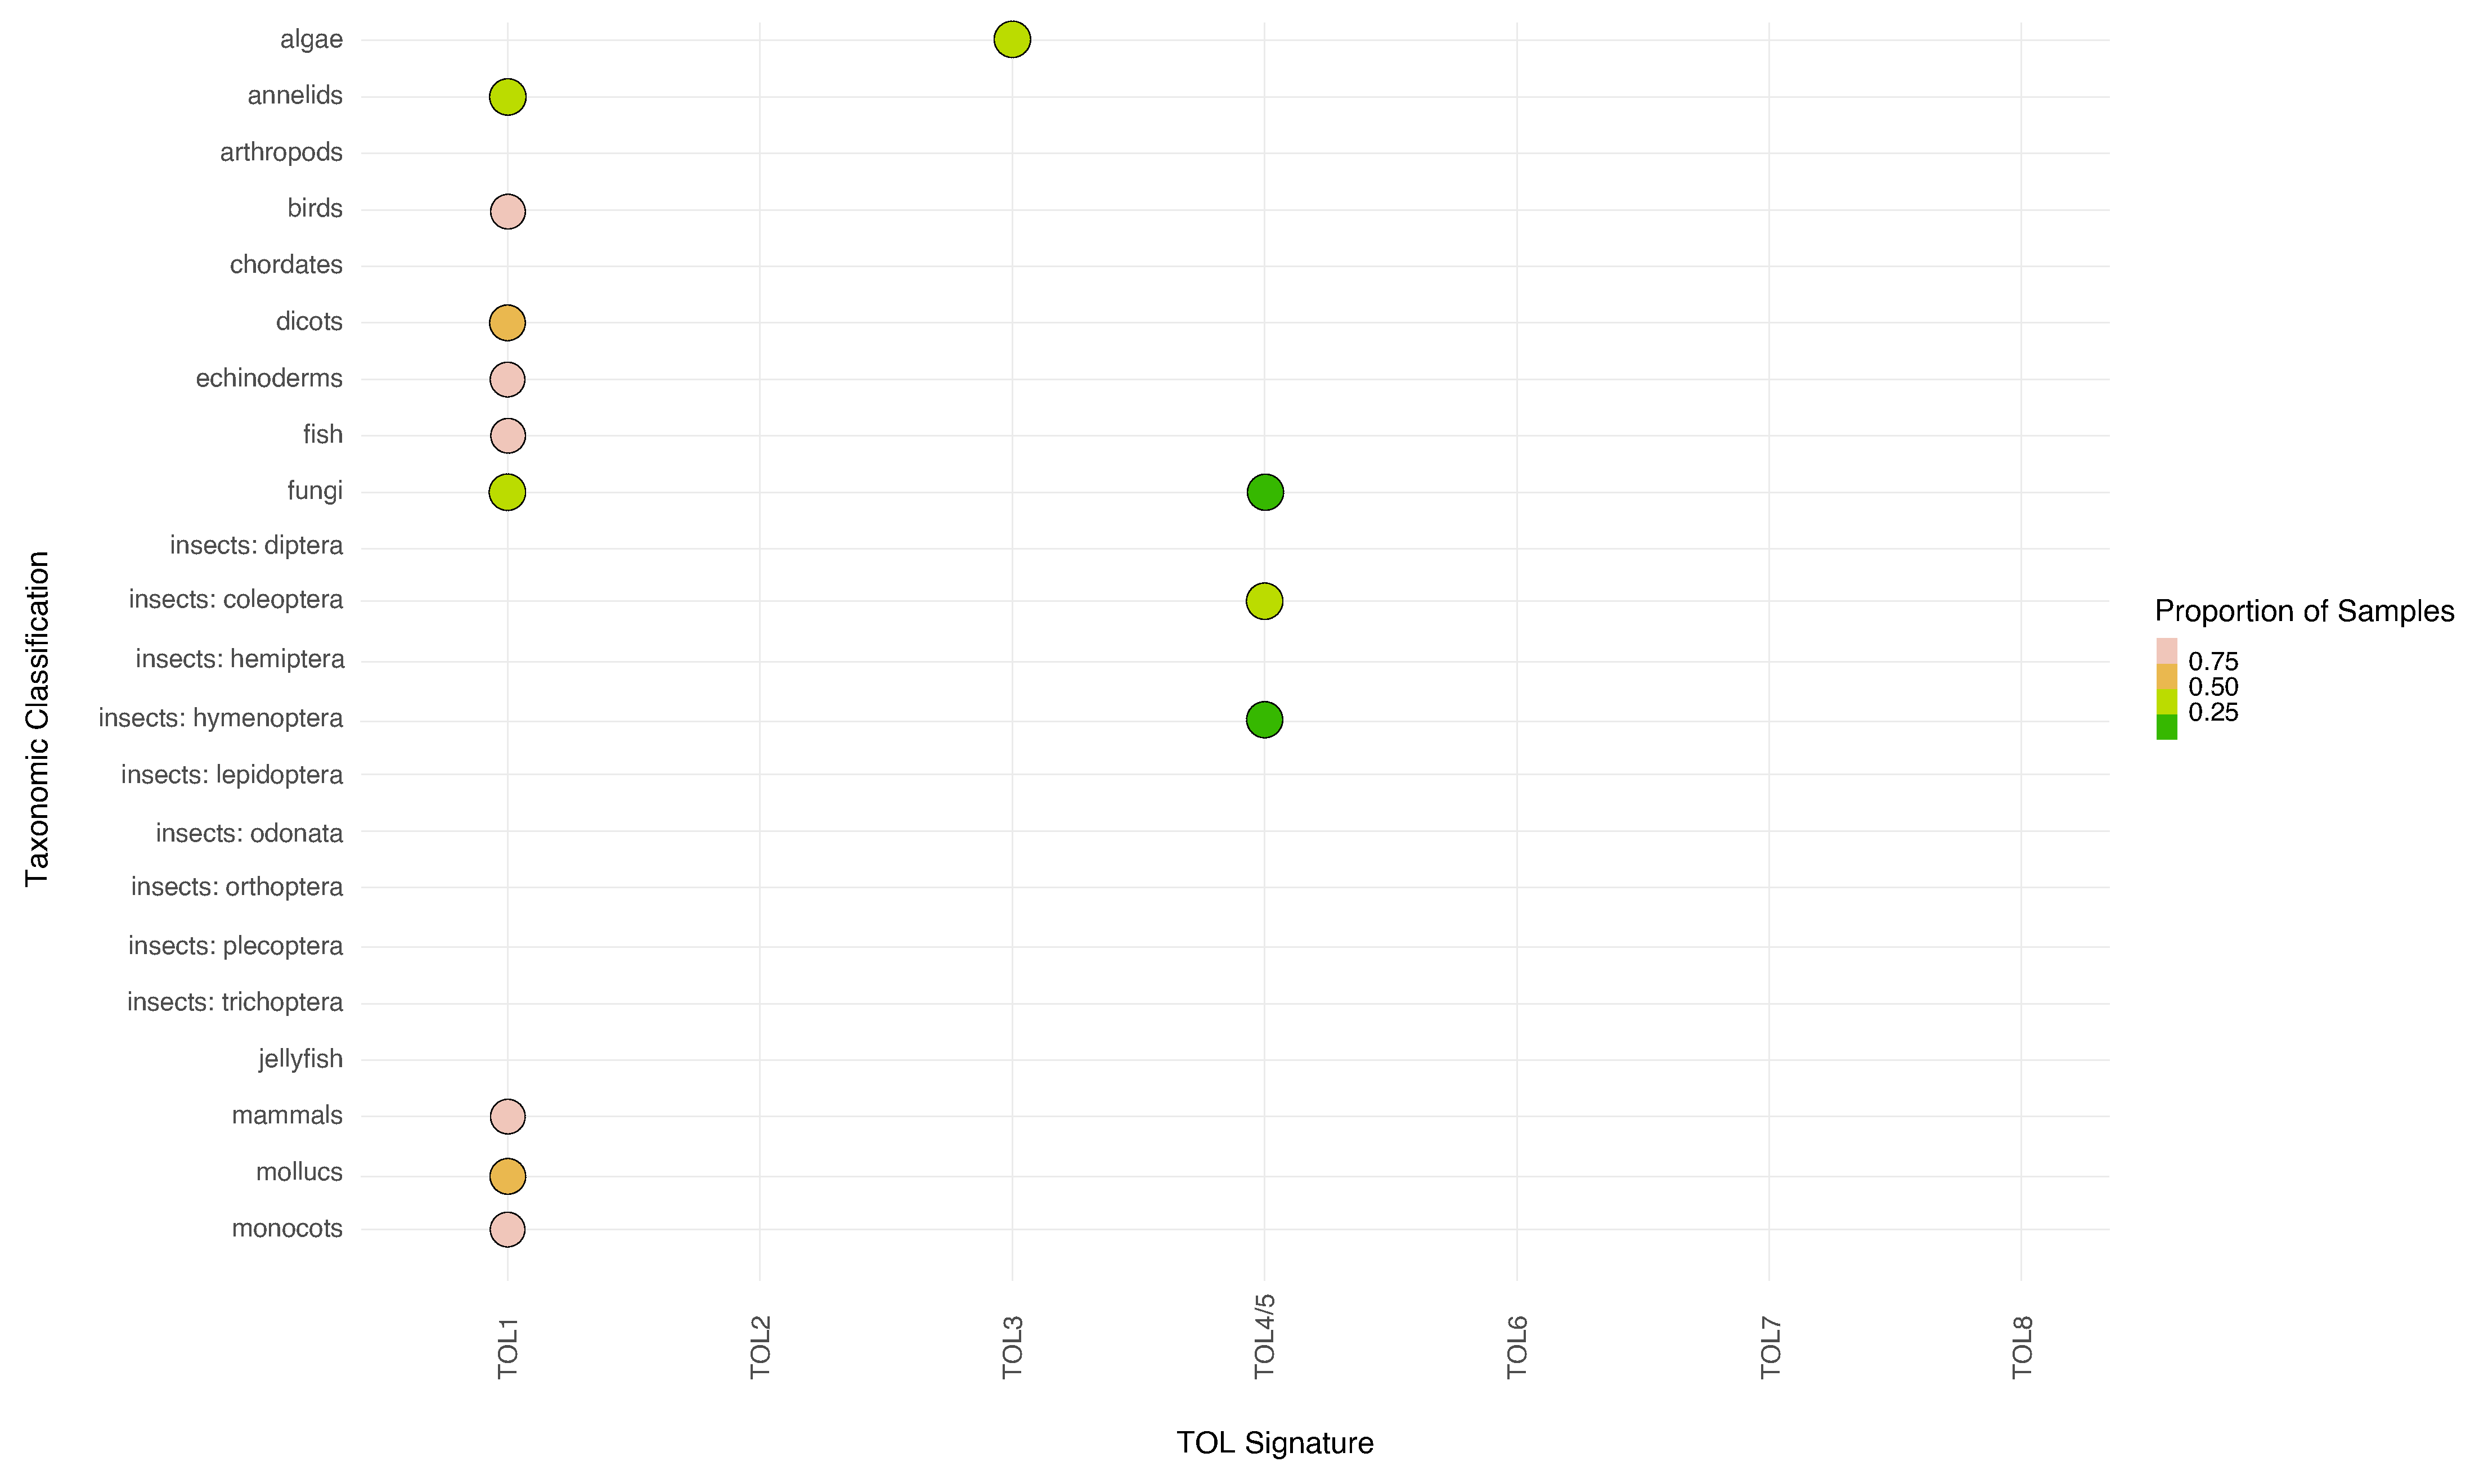
\includegraphics[width=\textwidth]{Vector/dtol_all_edited_tol_signature_presence_in_germline.pdf}
\end{centering}
\end{figure}

\pagebreak

\subsubsection{CCS error signatures}

In chapter 2, false positive mutations associated with inaccurate BQ score estimation were described in section \ref{sec:CCS-base-quality-score-recalibration} and was identified as a common error signature in DToL samples (Figure \ref{figure:E1}). The additional error processes described here are thought to be from library errors, which damage or incorrectly repair both the forward and reverse strands. 

\begin{figure}[htbp!]
\caption{Error signature 1 (E1)}
\label{figure:E1}
\begin{centering}
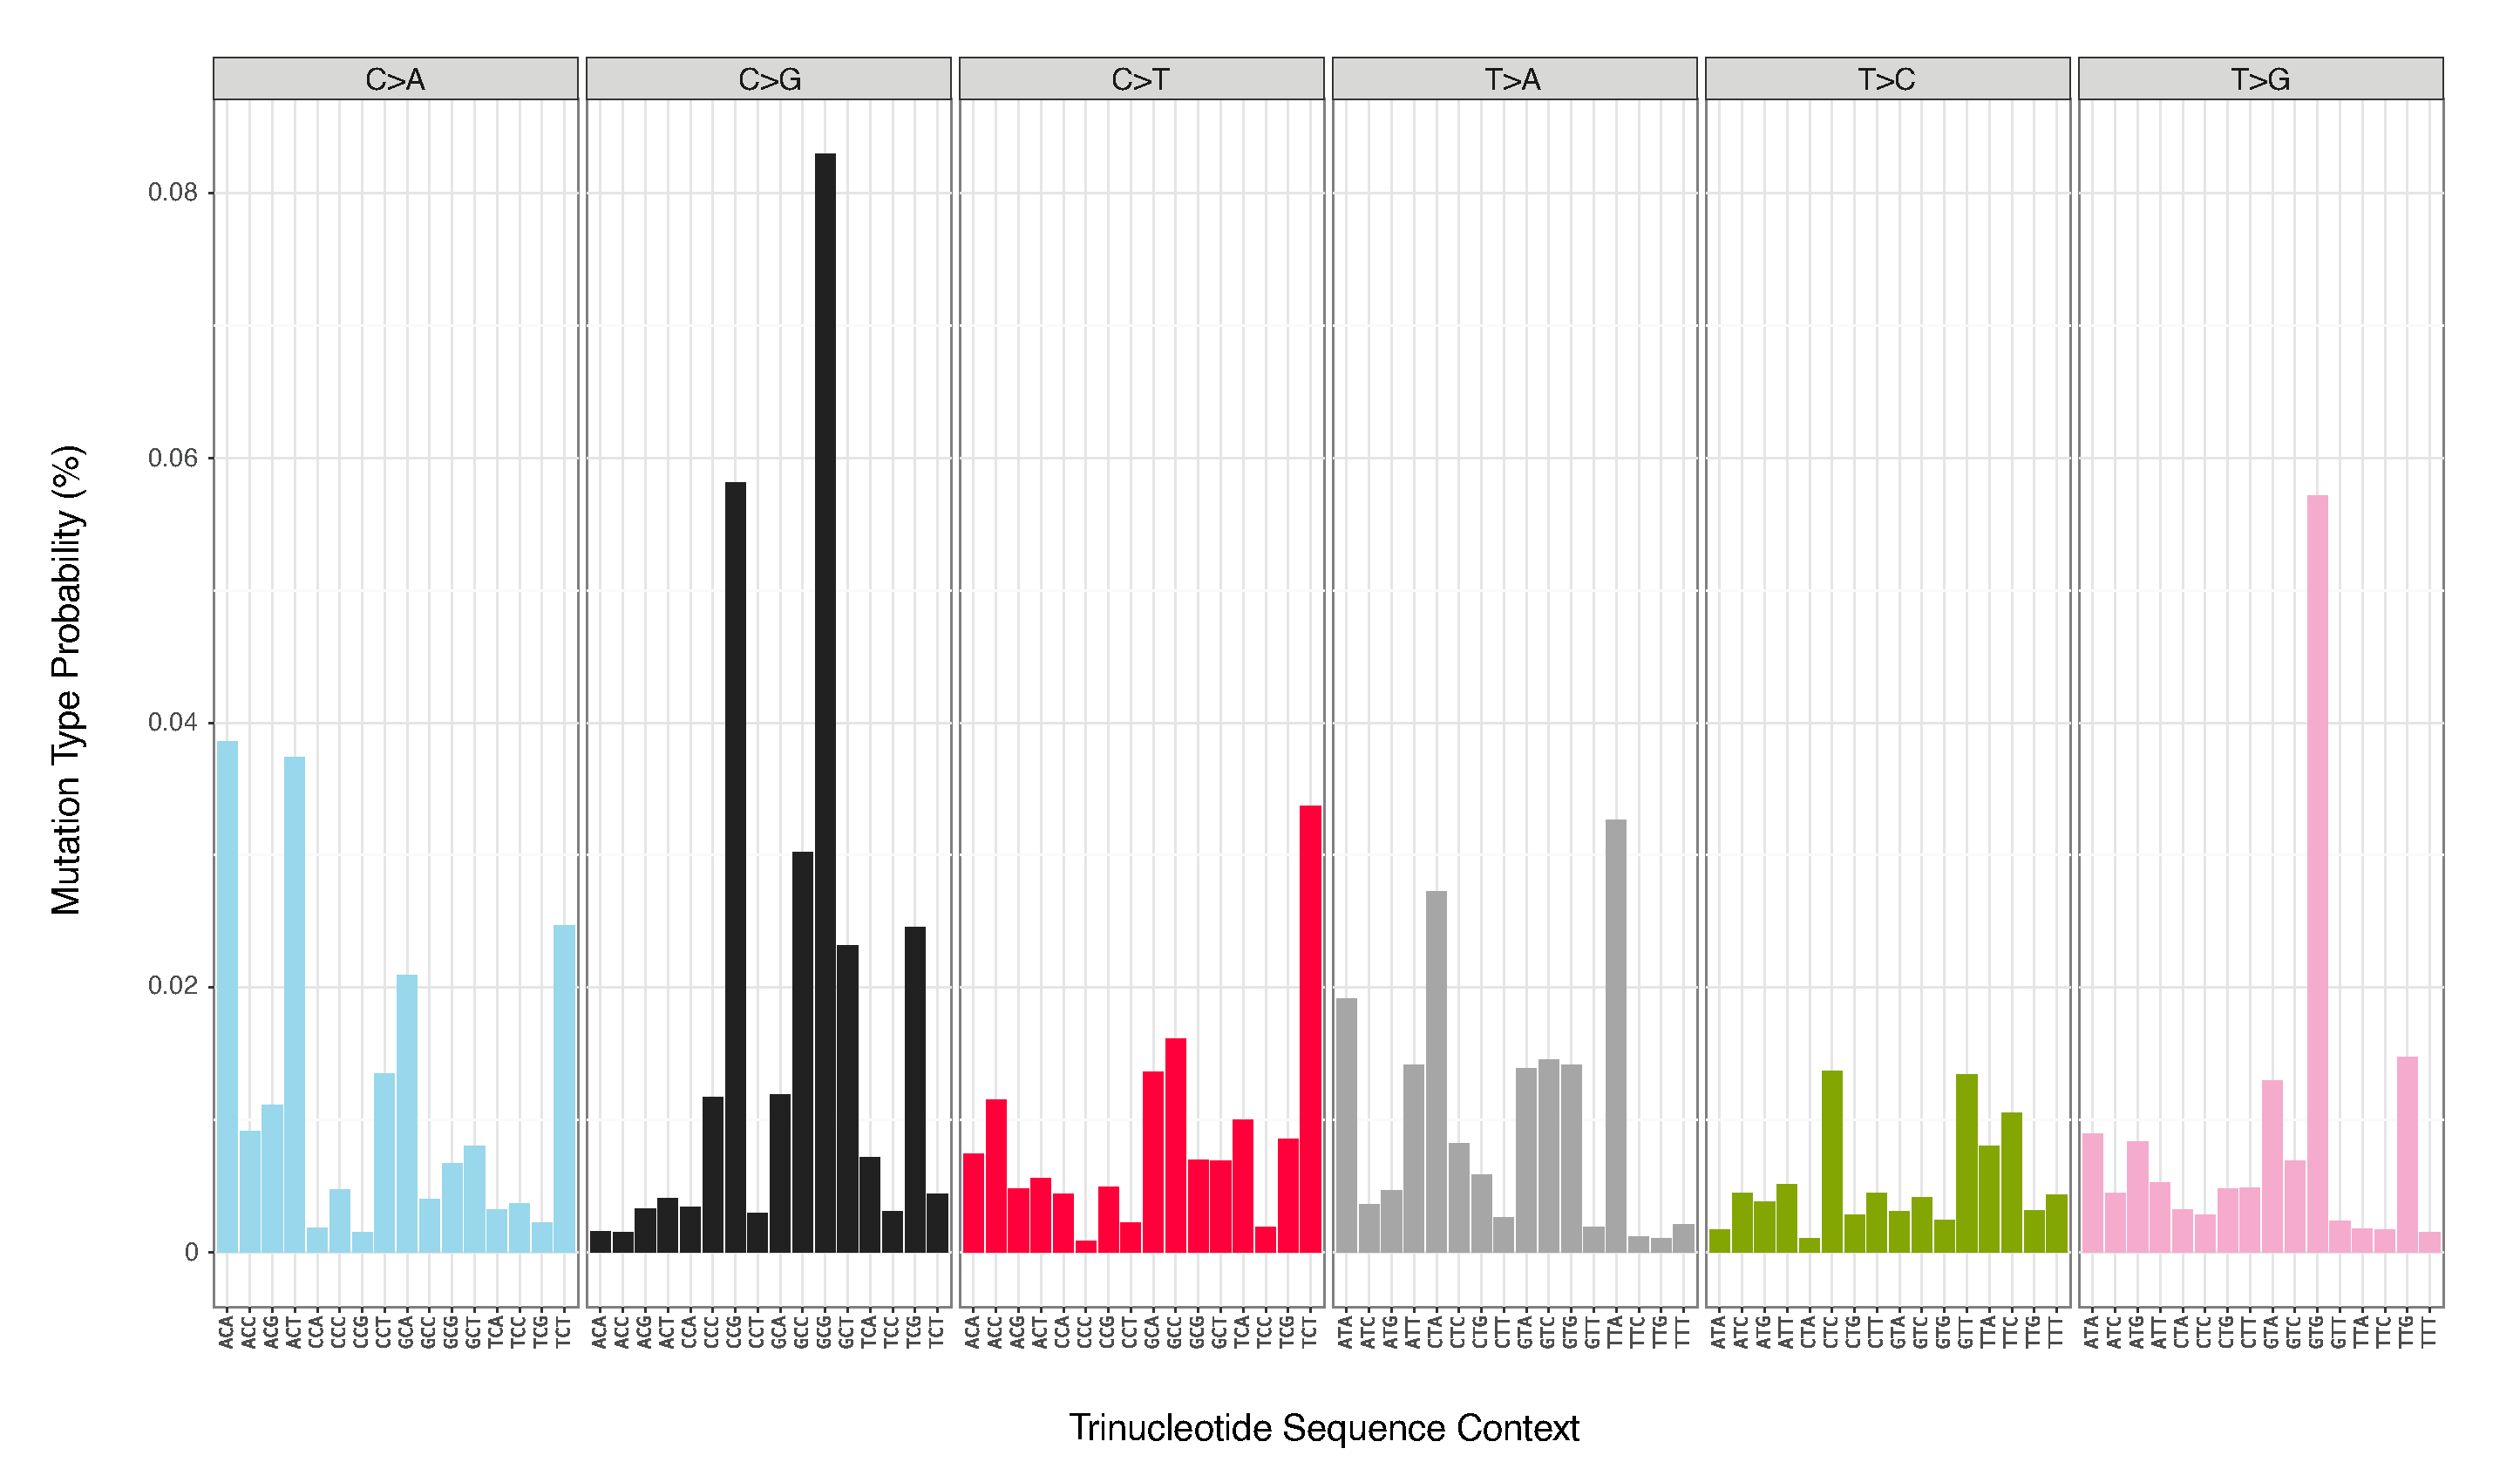
\includegraphics[width=\textwidth]{Vector/E1_signature.pdf}
\end{centering}
\end{figure}

The somatic mutational spectra in \textit{E. aenea} (riffle beetle) and \textit{T. trachurus} (atlantic horse mackerel) provide a canonical example of how library or sequencing errors manifests as somatic mutations (Figure \ref{figure:icElmAene2-fTraTra1}). The number of somatic mutations detected in these samples is many times greater than the median number of somatic mutations detected in the same eukaryotic lineage. Moreover, there is a notable dissimilarity between the germline and somatic mutational spectra, suggesting that two independent processes are active in the germline and the soma. In contrast, in \textit{H. sapiens}, somatic mutational processes generating the SBS1 and SBS5 COSMIC mutational signatures are active in both the germline and the soma \cite{Moore2021-dl}. These observations suggests that the observed mutational spectra are a result of either library or sequencing errors.  

\begin{figure}[h!]
\caption{Germline and somatic mutational spectra in \textit{E. aenea} and \textit{T. trachurus}}
\label{figure:icElmAene2-fTraTra1}
\begin{centering}
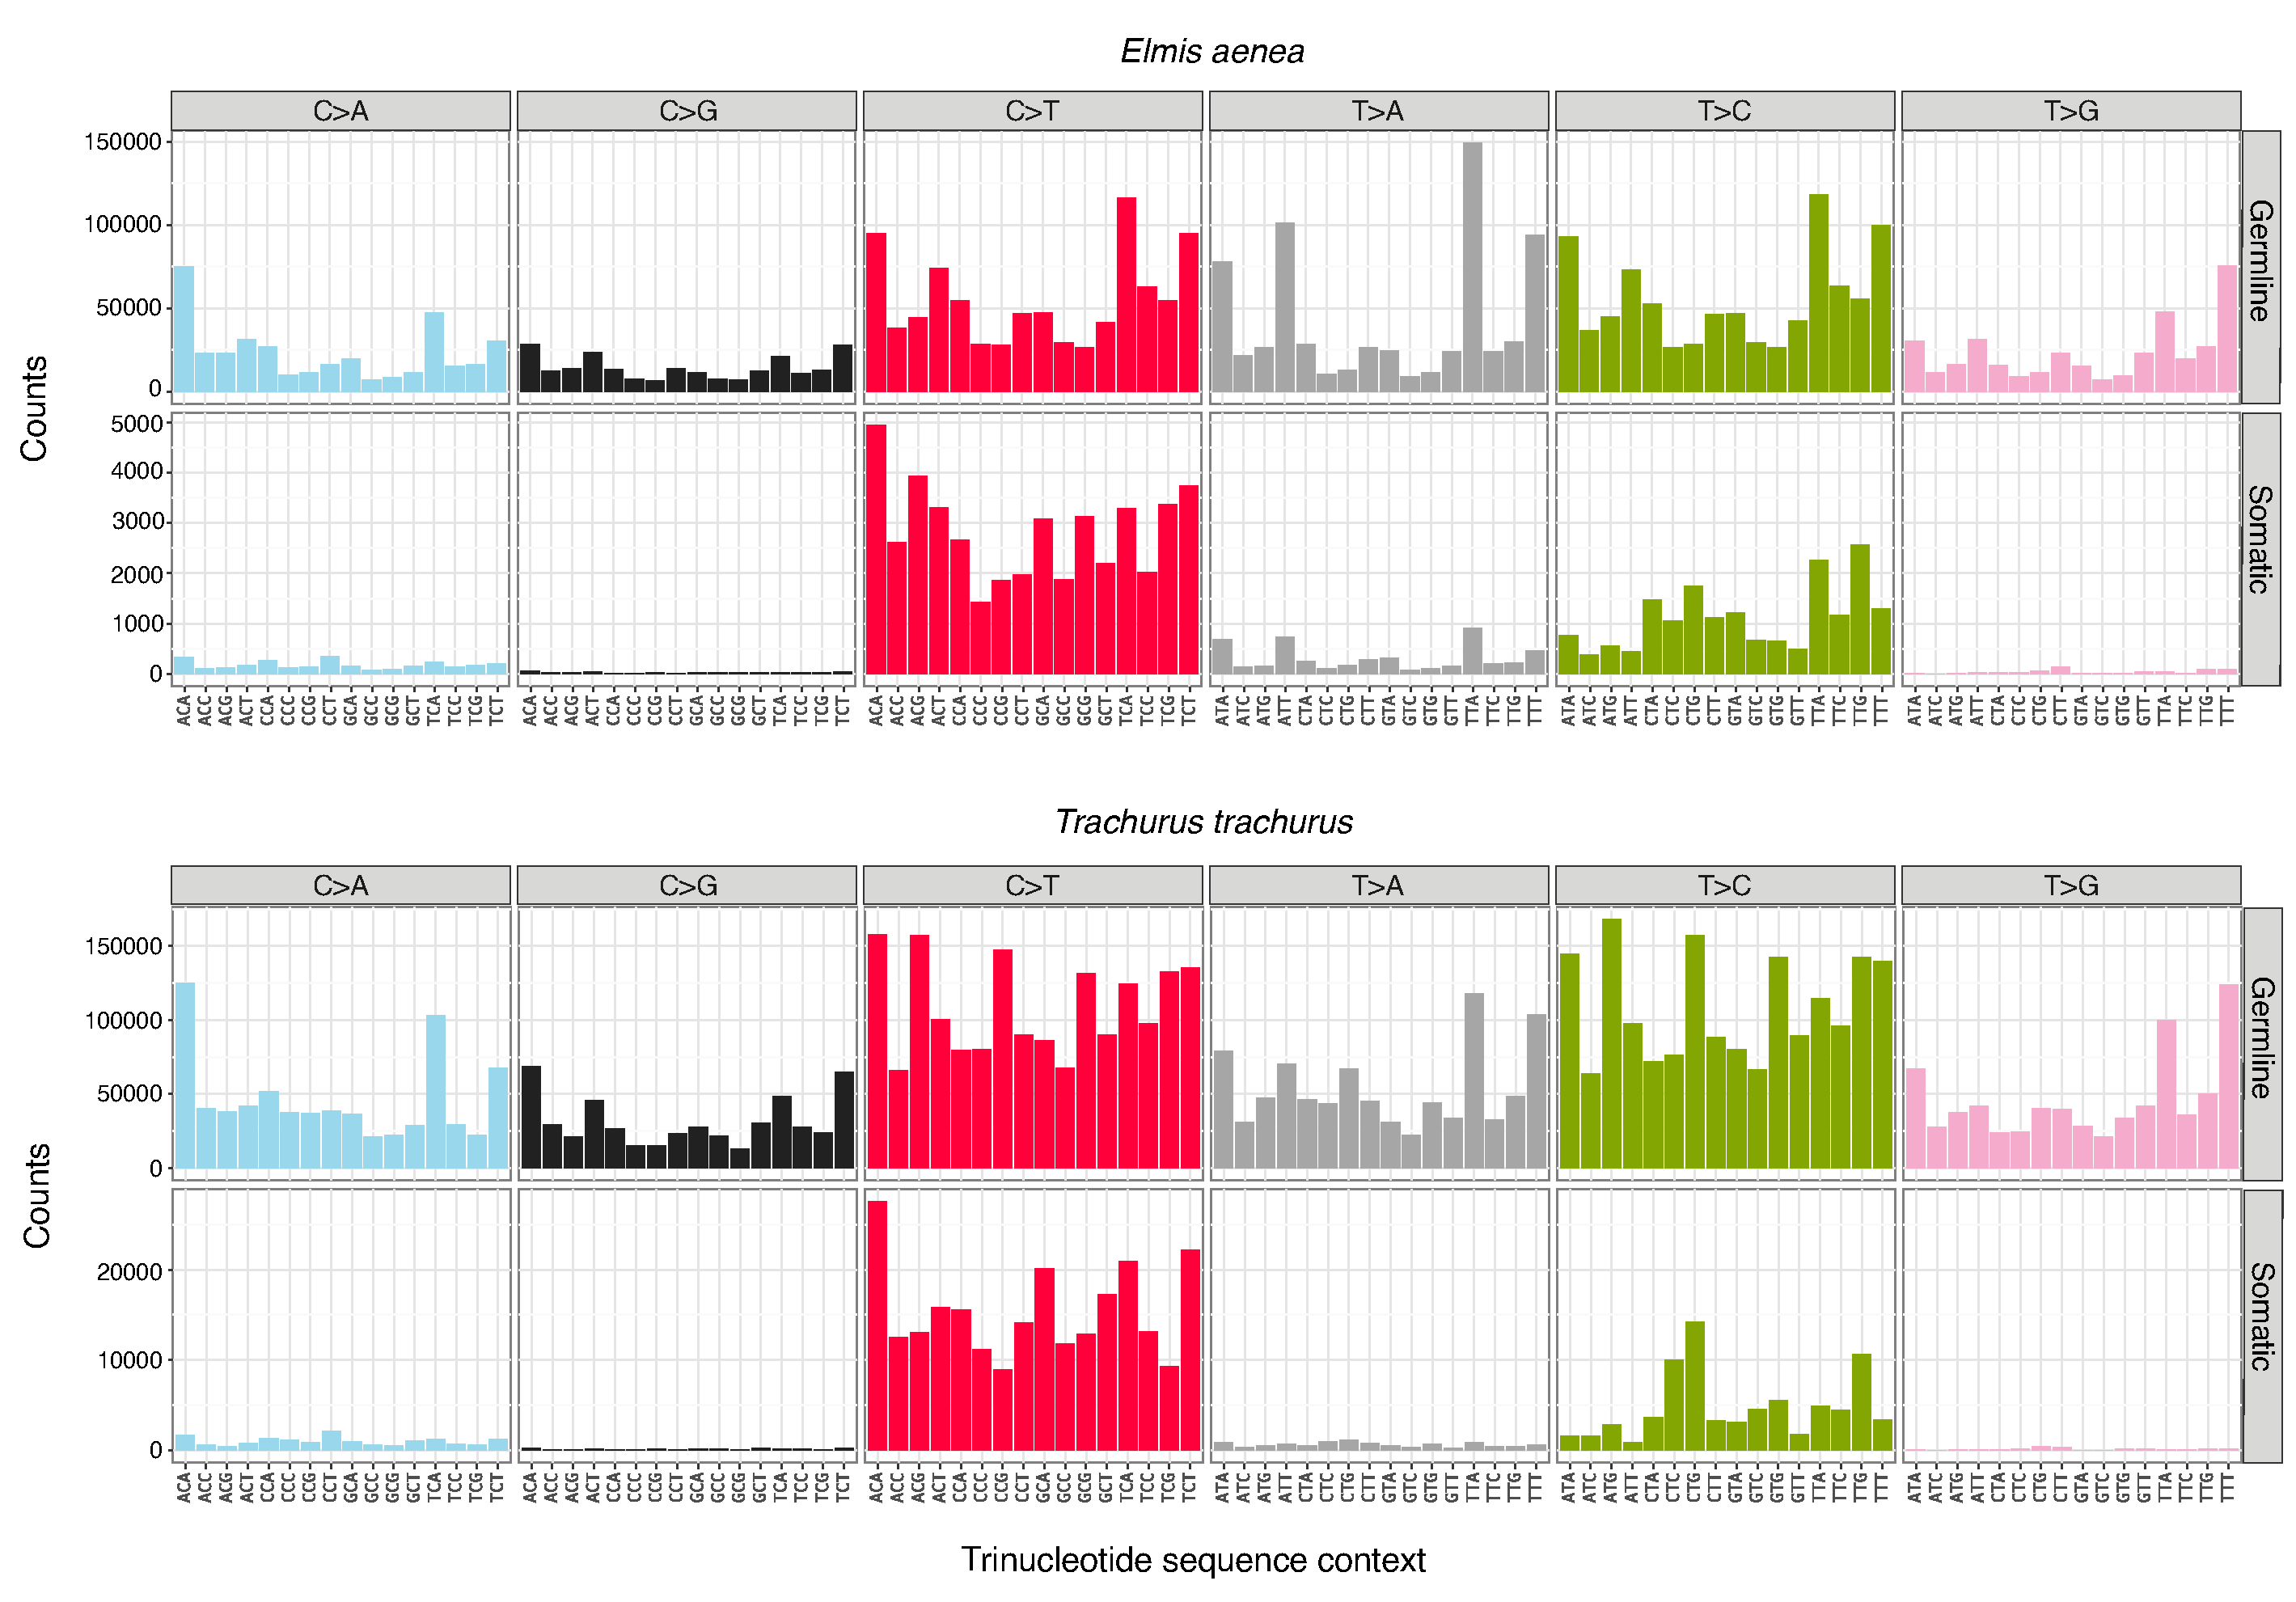
\includegraphics[width=\textwidth]{Vector/icElmAene2_fTraTra1.germline_somatic_sbs96.pdf}
\end{centering}
\end{figure}

The somatic mutational spectra observed in \textit{E. aenea}, \textit{T. trachurus} and other samples were identified and designated as an error signature 2 (E2) (Figure \ref{figure:E2}). C>T and T>C somatic mutations in all trinucleotide sequence contexts are prominent features of the E2 signature, with a greater contribution from C>T somatic mutations and smaller contributions from other base substitution classes. 

\begin{figure}[htbp!]
\caption{Error signature 2 (E2)}
\label{figure:E2}
\begin{centering}
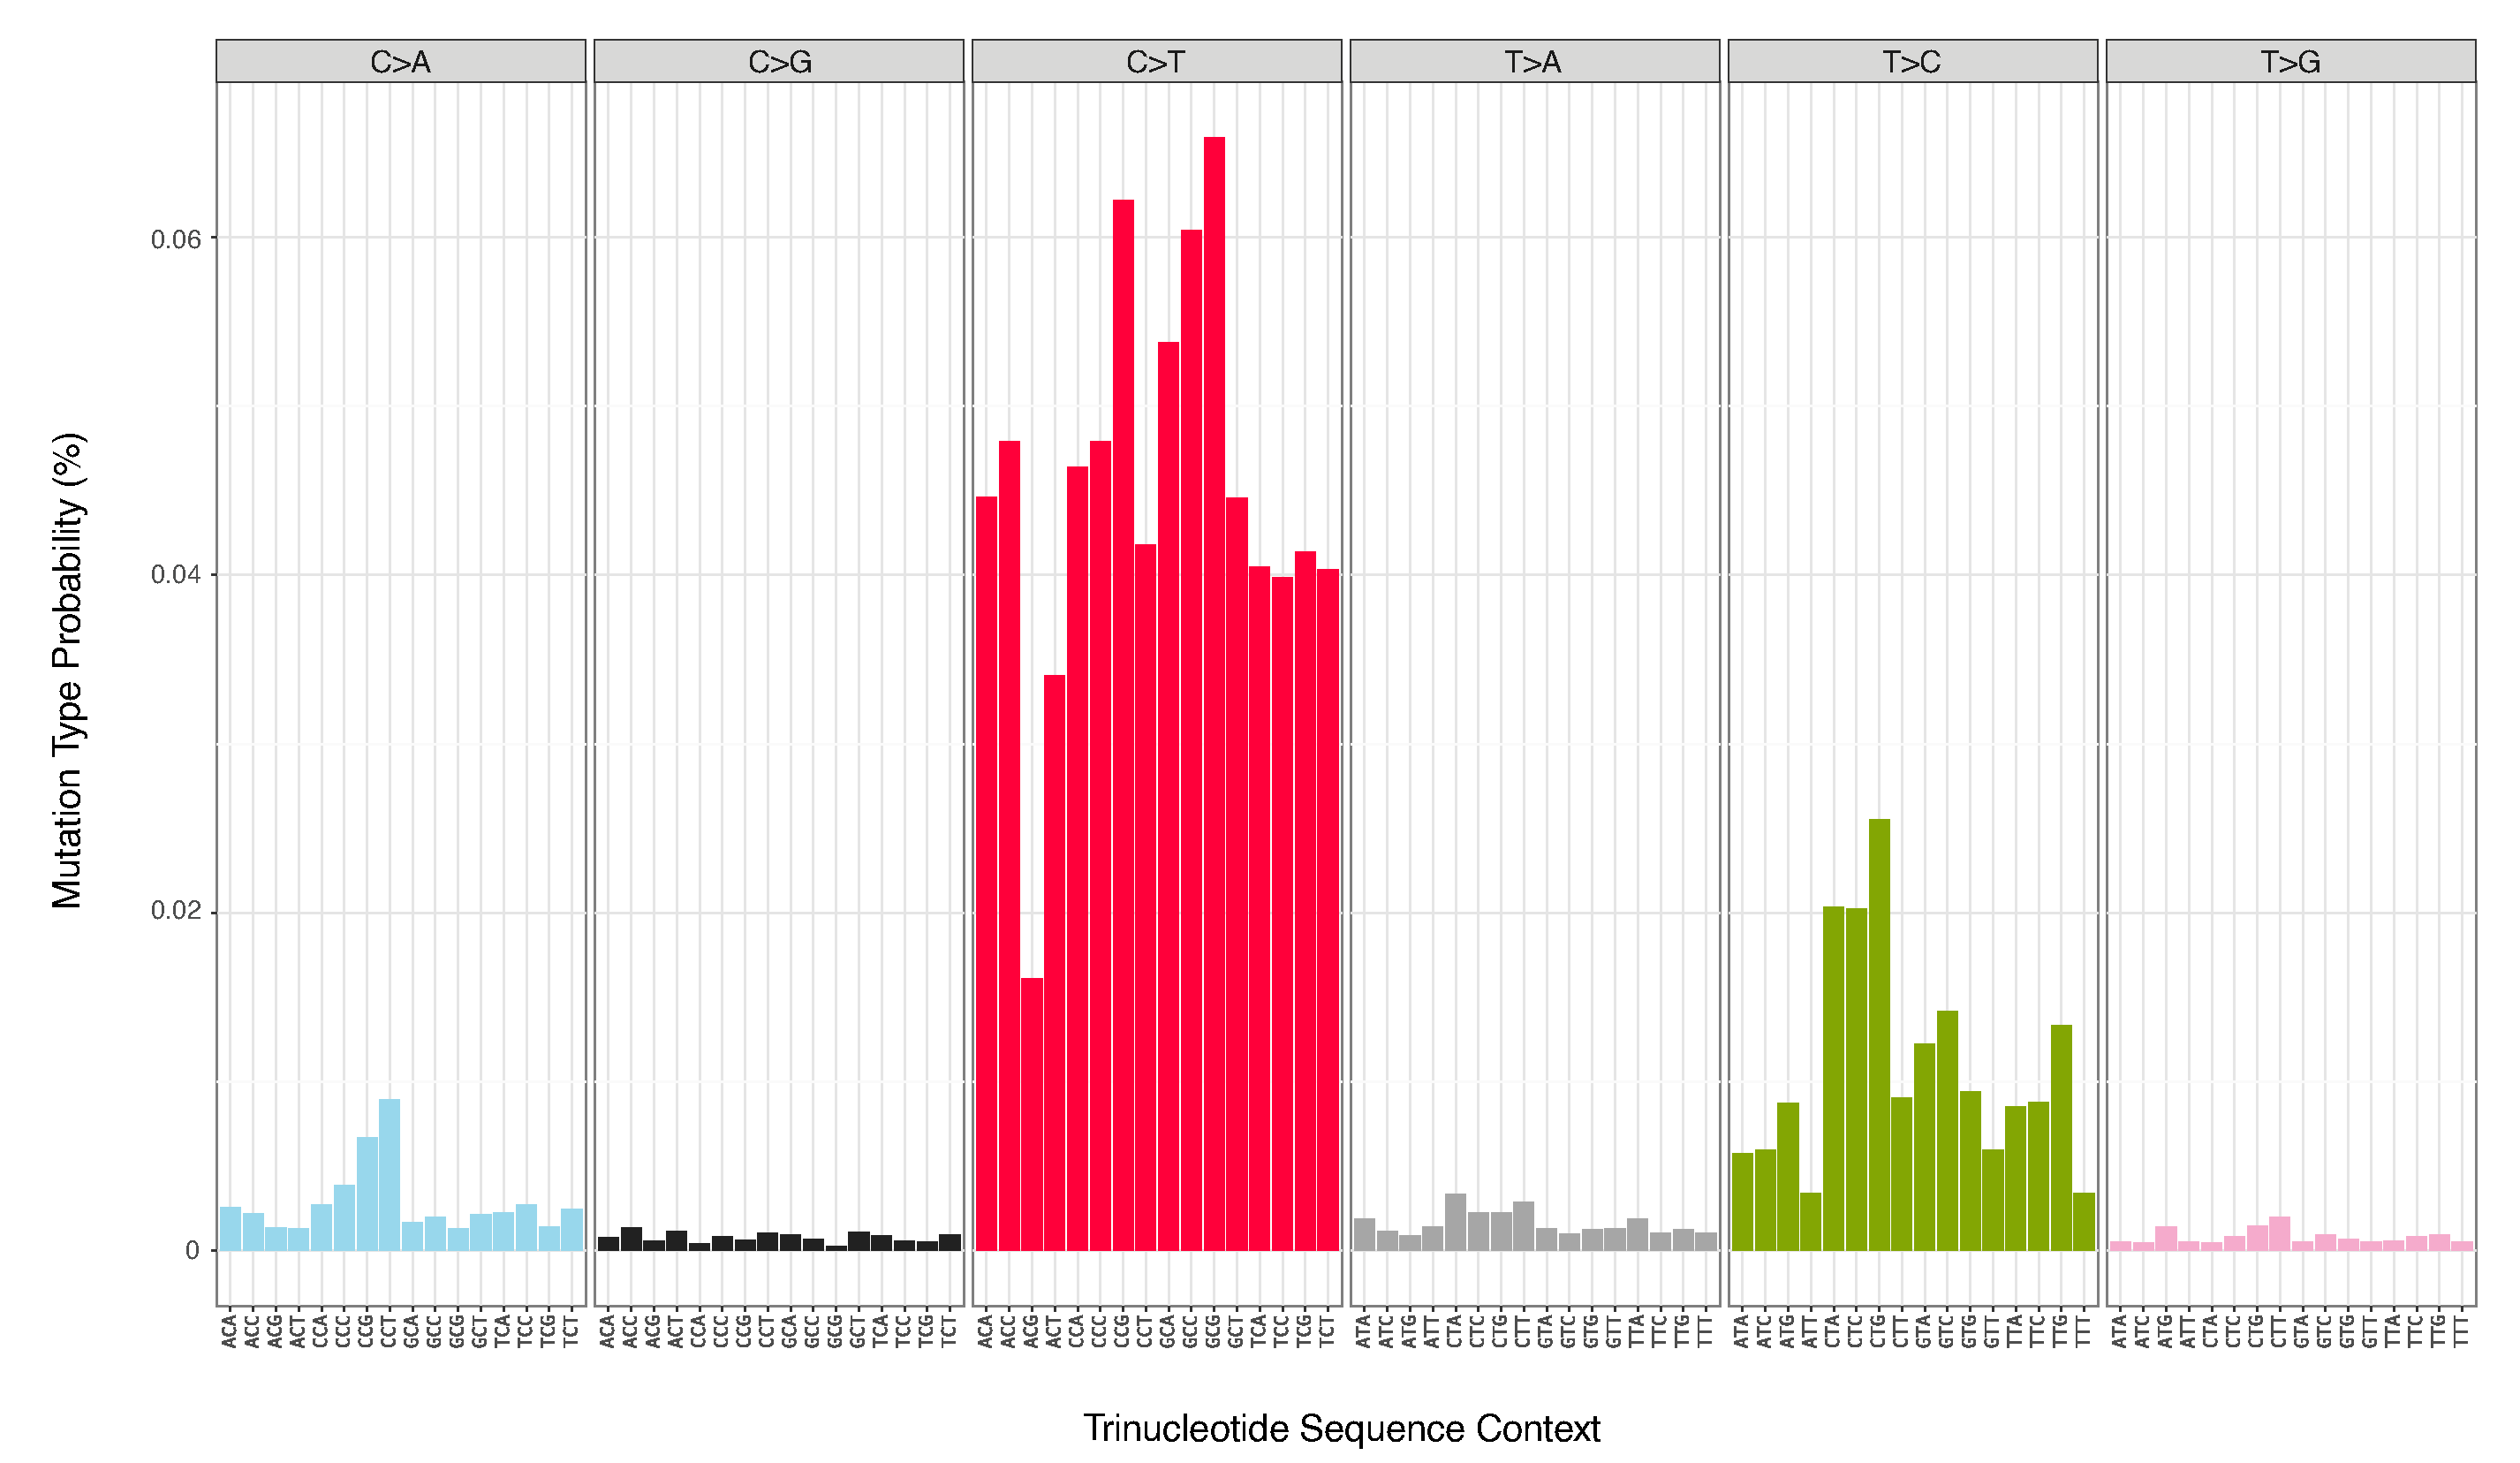
\includegraphics[width=\textwidth]{Vector/E2_signature.pdf}
\end{centering}
\end{figure}

Here, I hypothesise that the E2 error signature is derived from a library error that affects both strands of a double-stranded DNA molecule. The following observations regarding the pbccs algorithm support this hypothesis. Although the pbccs algorithm documentation does not describe how the BQ score is calculated and assigned \cite{ccs2023}, it implies that a Q93 BQ score is assigned to a CCS base only when both forward and reverse strand subreads support the CCS base. If DNA damage or modification occurs only on one of the strands, the pbccs algorithm detects the non-complementary base pairing as a heteroduplex and assigns a low BQ score to the CCS base. Moreover, the subread error rate of 10 to 15\% \cite{Chaisson2012-vr} suggests that a minimum of 10 subreads is necessary to generate a Q93 CCS base. Furthermore, as sequencing errors are believed to be random, the probability of a DNA polymerase (DNAP) introducing the same error to multiple subreads during strand-displacement synthesis is infinitesimally small. The alternative explanation is that both the forward and reverse strand of a template molecule is damaged, the damage is incorrectly repaired, the resulting mismatch is incorporated into the consensus sequence and called as a somatic mutation. 

The cause of the library errors is currently unknown. However, the E2 signature is synthetic in nature, as specific library preparation processes are thought to be responsible for the DNA damage and the incorrect repair. Systematic elimination and examination of DNA damage and repair steps should facilitate the identification of the primary causes of library errors and help find solutions to address the issue. 

\subsubsection{TOL mutational signatures}

Here, I describe mutational signatures that are a component of both germline and somatic mutational spectra. I also present mutational signatures where somatic mutational processes with transcriptional-strand bias is responsible for generating the identified mutational signature. Hence, germline-only mutational signatures and somatic mutational signatures with insufficient biological evidence have been excluded from the analysis. 

If the mutational signature is present in both the germline and soma, both somatic and germline mutations are shown under the SBS96 and SBS52 classification system, respectively. In addition, the conservation of these mutational signatures across the different eukaryotic lineages allow us to time the emergence of somatic mutational processes that generated these mutational signatures (Figure \labelcref{figure:tol-soma,figure:tol-germline}).

\begin{description}
    \item[TOL1 signature]
\end{description}

The TOL1 signature is found throughout the Plant, Animal, and Fungi kingdom and C>T mutations at CG dinucleotide sequence contexts is the predominant feature of the mutational signature (Figure \ref{figure:TOL1}). Considering the high similarity (0.XXX) between the TOL1 and COSMIC SBS1 signature, the aetiology of the TOL1 signature is believed to be the spontaneous deamination of 5-methylcytosine to thymine. The presence of the TOL1 signature in these three kingdoms suggests that cytosine methylation in CG dinucleotides may have occurred in the most recent common ancestor of these three eukaryotic lineages, or that it has evolved independently in each of these lineages. The conservation of DNA methyltransferase 1 (DNMT1), which is responsible for methylation of cytosine in CG dinucleotides, in eukaryotic lineages from these 3 kingdoms corroborates our observation \cite{De_Mendoza2019-dy, Mattei2022-fm}. If DNA methylation has occurred in the most recent common ancestor of these eukaryotic lineages, somatic mutational process associated with the TOL1 signature is thought to have first appeared approximately 1.6 billion years ago \cite{Wang1999-vj, Heckman2001-ty}

\begin{description}
    \item[TOL2 signature]
\end{description}

The TOL2 signature is more commonly found in vascular plants (dicots and monocots) (Figure \ref{figure:tol-soma}) and is characterised by the prominence of C>A and C>T mutations (Figure \ref{figure:TOL2}). Intriguingly, C>T mutations are absent from trinucleotide sequence contexts with CG dinucleotides. Plants are well known to show wider patterns of DNA methylation. CMT3 is responsible for cytosine methylation at CHG sequence context while DRM2 is responsible for cytosine methylation at CHH Sequence contexts where H can be A, C or T bases \cite{Finnegan1998-qp}. One possible hypothesis for C>T mutations is the spontaneous deamination of 5-methylcytosine to thymine in CHG and CHH sequence contexts.

One possible source of C>A mutation is oxidative DNA damage. Reactive oxygen species produced during photosynthesis could be the source of DNA damage. As discussed in section \ref{sec:somatic_mutation_detection_in_tumours}, oxidation of guanine generates 8-oxo-guanine (8-oxoG) and 8-oxoG preferentially binds to adenine instead of cytosine, which leads to C:G>A:T somatic mutations. Considering the conservation of this mutational signature in both dicots and monocots, somatic mutational processes associated with TOL2 signature are estimated to have emerged approximately 200 million years ago when the Plant and Animal/Fungi kingdom have diverged \cite{Wolfe1989-pg}. 

\begin{description}
    \item[TOL3 signature]
\end{description}

The TOL3 signature is characterised primarily by C>A and C>G somatic mutations at ACA trinucleotide. In addition, C>T somatic mutations at ACA and GCG trinucleotide are counterbalanced by T>C somatic mutations at ATA and GTG trinucleotides. Fascinatingly, somatic mutational process that generates the TOL3 signature is solely present within the order Perciformes (Taurulus bubalis (bony fishes) and Pholis gunnellus (rock gunnel)), an order of ray-finned fish, but not in the order Cypriniformes (Barbus barbus (barbel) and Barbatula barbatula (stone loach)) (Fig \ref{figure:TOL3}). Given the limited number of samples in the superclass Osteichthyes (ray-finned fishes), further investigation is necessary to determine whether TOL3 signature is unique to Perciformes. 

\begin{description}
    \item[TOL4 signature]
\end{description}

The TOL4 signature is enriched with C>T somatic mutations at CCN and TCN trinucleotides with dipyrimidines (Figure \ref{figure:TOL4}) is exclusively found in Algae, Coleoptera, Diptera and Hymenoptera. The TOL4 signature shows the highest similarity to COSMIC SBS7ab signature (cosine similarity: 0.83, 0.64), which is known to be caused UV light induced DNA damage \cite{Nik-Zainal2015-bj}. The exposure to UV light leads to the generation of cyclobutane pyrimidine dimers (CPD) at dipyrimidine sites and subsequent deamination of CPD dimers produces C>T and CC>TT somatic mutations \cite{Jin2021-ae}. In addition, COSMIC SBS7ab exhibits transcriptional strand bias where C>T mutations are enriched on the un-transcribed strand compared to the transcribed strand. 

As \textit{D. primolecta} (green algae) requires sunlight photosynthesis, somatic mutations attributable to the TOL4 signature in \textit{D. primolecta} are most likely the result of UV light-induced DNA damage. In contrast, an alternative mechanism is hypothesised to be active in insects. This is because the somatic mutational process that generates the TOL4 signature in insects is active in both the germline and the soma, and UV light is unlikely to damage the germline stem cells in insects.

\begin{description}
    \item[TOL5 signature]
\end{description}

The TOL5 signature is a variant of the TOL4 signature with C>T at CCN and TCN trinucleotides and T>C somatic mutations at CTN and TTN trinucleotides with dipyrimidines (Figure \ref{figure:TOL5}). The probability of C>T and T>C somatic mutations is balanced in the TOL5 signature. However, in the samples where somatic mutational processes associated with the TOL4 and TOL5 signature are active, C>T and T>C somatic mutations are asymmetrically distributed (Figure \ref{figure:iyAthRosa1-SBS96-SBS192}).

%\begin{figure}[h!]
%\caption{Somatic mutational spectra in \textit{Athalia rosae} (coleseed sawfly)}
%\label{figure:iyAthRosa1}
%\begin{centering}
%\makebox[\textwidth][c]{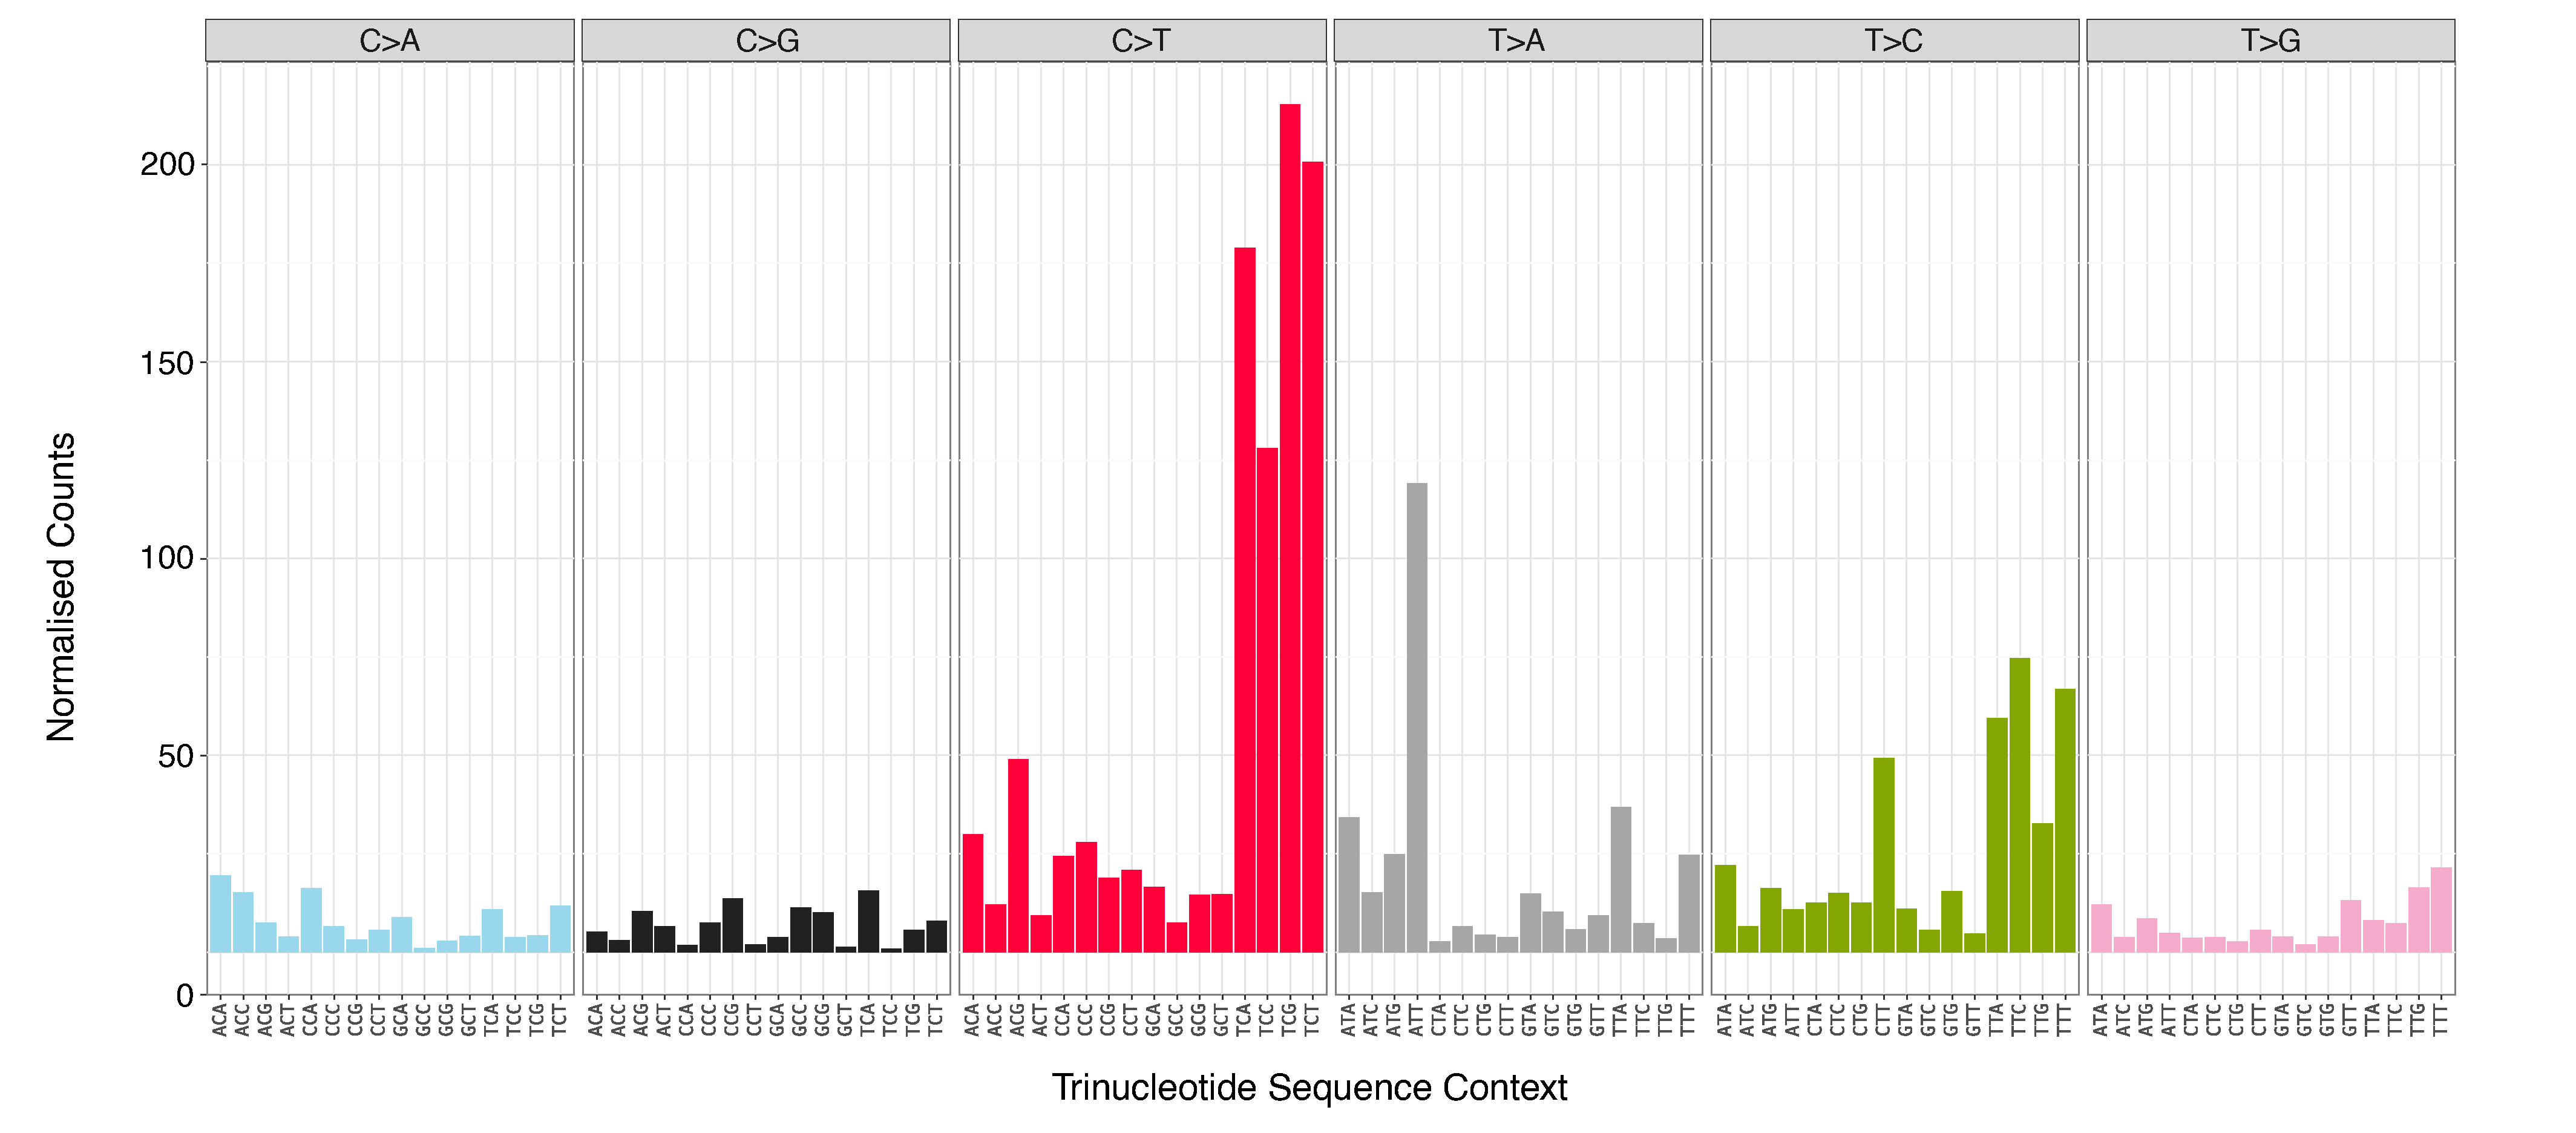
\includegraphics[width=1\textwidth]{Vector/iyAthRosa1.somatic_sbs96.pdf}}
%\end{centering}
%\end{figure}

Unlike COSMIC 7ab signature, the somatic mutations responsible for the TOL5 signature are equally distributed on both the transcribed and untranscribed strand, providing further evidence that another somatic mutational process is associated with the TOL5 signature (Figure \ref{figure:iyAthRosa1-SBS96-SBS192}).

The TOL4 and TOL5 signatures are an interesting example where analysing both germline and somatic mutational processes helps us recognise that C>T somatic mutations identified in the germline TOL4/5 signature exhibit strand asymmetry with C>T and T>C somatic mutations. As the ancestral allele is unknown for germline mutations, C>T and T>C germline mutations are indistinguishable, and their counts are summed together. However, the ancestral allele is known for somatic mutations, and therefore C>T and T>C strand asymmetry is observed in the somatic mutational signature. By transforming the TOL4/5 somatic mutational signature from the SBS96 classification system to the SBS52 classification system and comparing it to the TOL4/5 germline mutational signature, it becomes apparent that the same somatic mutational process generates the germline and somatic mutational signature (Figure \ref{figure:TOL5-somatic-germline}). 

\begin{description}
    \item[TOL6/7 signature]
\end{description}

The TOL6 signature is defined by C>A, C>G, and C>T somatic mutations at ACA and TCT trinucleotides and C>T and T>C somatic mutations at ANA, CNC, CNT, TNC and TNT trinucleotides where N is a pyrimidine base (Figure \ref{figure:TOL6}). The TOL7 signature is highly similar to the TOL6 signature with additional C>A and C>G somatic mutations at ACT trinucleotides and C>T and T>C somatic mutations at GNC trinucleotides (Figure \ref{figure:TOL7}). The TOL6 signature is exclusively found in Hymenoptera while the TOL7 signature is found in both Diptera and Coleoptera. 

\begin{description}
    \item[TOL8 signature]
\end{description}

The TOL8 signature is enriched with C>A somatic mutations at either NCG or GCN trinucleotides (Figure \ref{figure:TOL8}). In addition, the TOL8 signature exhibits transcriptional-strand bias, where somatic mutations are preferentially acquired on the transcribed strand, indicating that the somatic mutations are a result of transcription-coupled damage. Moreover, the TOL8 signature is a prominent feature in the somatic mutational spectra of \textit{Syritta pipiens} (thick-legged hoverfly) (Figure \ref{figure:idSyrPipi1-SBS96-SBS192}).

\pagebreak

\begin{description}
    \item[TOL9 signature]
\end{description}

TOL9/10 signature is characterised by C>T somatic mutations at CCN trinucleotides and is a major contributor to the somatic mutations present in \textit{Bombylius discolor} (dotted bee-fly) (Figure \labelcref{figure:TOL9,figure:TOL10}). Gene annotation is not available for \textit{B. discolor} to determine whether the TOL9/TOL10 signature exhibits transcriptional-strand bias and whether these signatures have similar characteristics as COSMIC SBS7ab signatures. 

\begin{description}
    \item[TOL11 signature]
\end{description}

The TOL11 is identified by C>A, C>G and C>T somatic mutations at ACA trinucleotides and some contributions from other base substitution classes (Figure \ref{figure:TOL11}). The TOL11 signature is uniquely present in \textit{Platycheirus albimanus} (white-footed hoverfly) and also exhibits transcriptional strand bias where the somatic mutations are enriched on the untranscribed strand, indicating that the somatic mutations on the transcribed strand are repaired through transcription-coupled repair (Figure \ref{figure:idPlaAlba1-SBS96-SBS192}). 

\begin{figure}[htbp!]
\caption{TOL signature 1 (TOL1)}
\label{figure:TOL1}
\begin{centering}
\makebox[\textwidth][c]{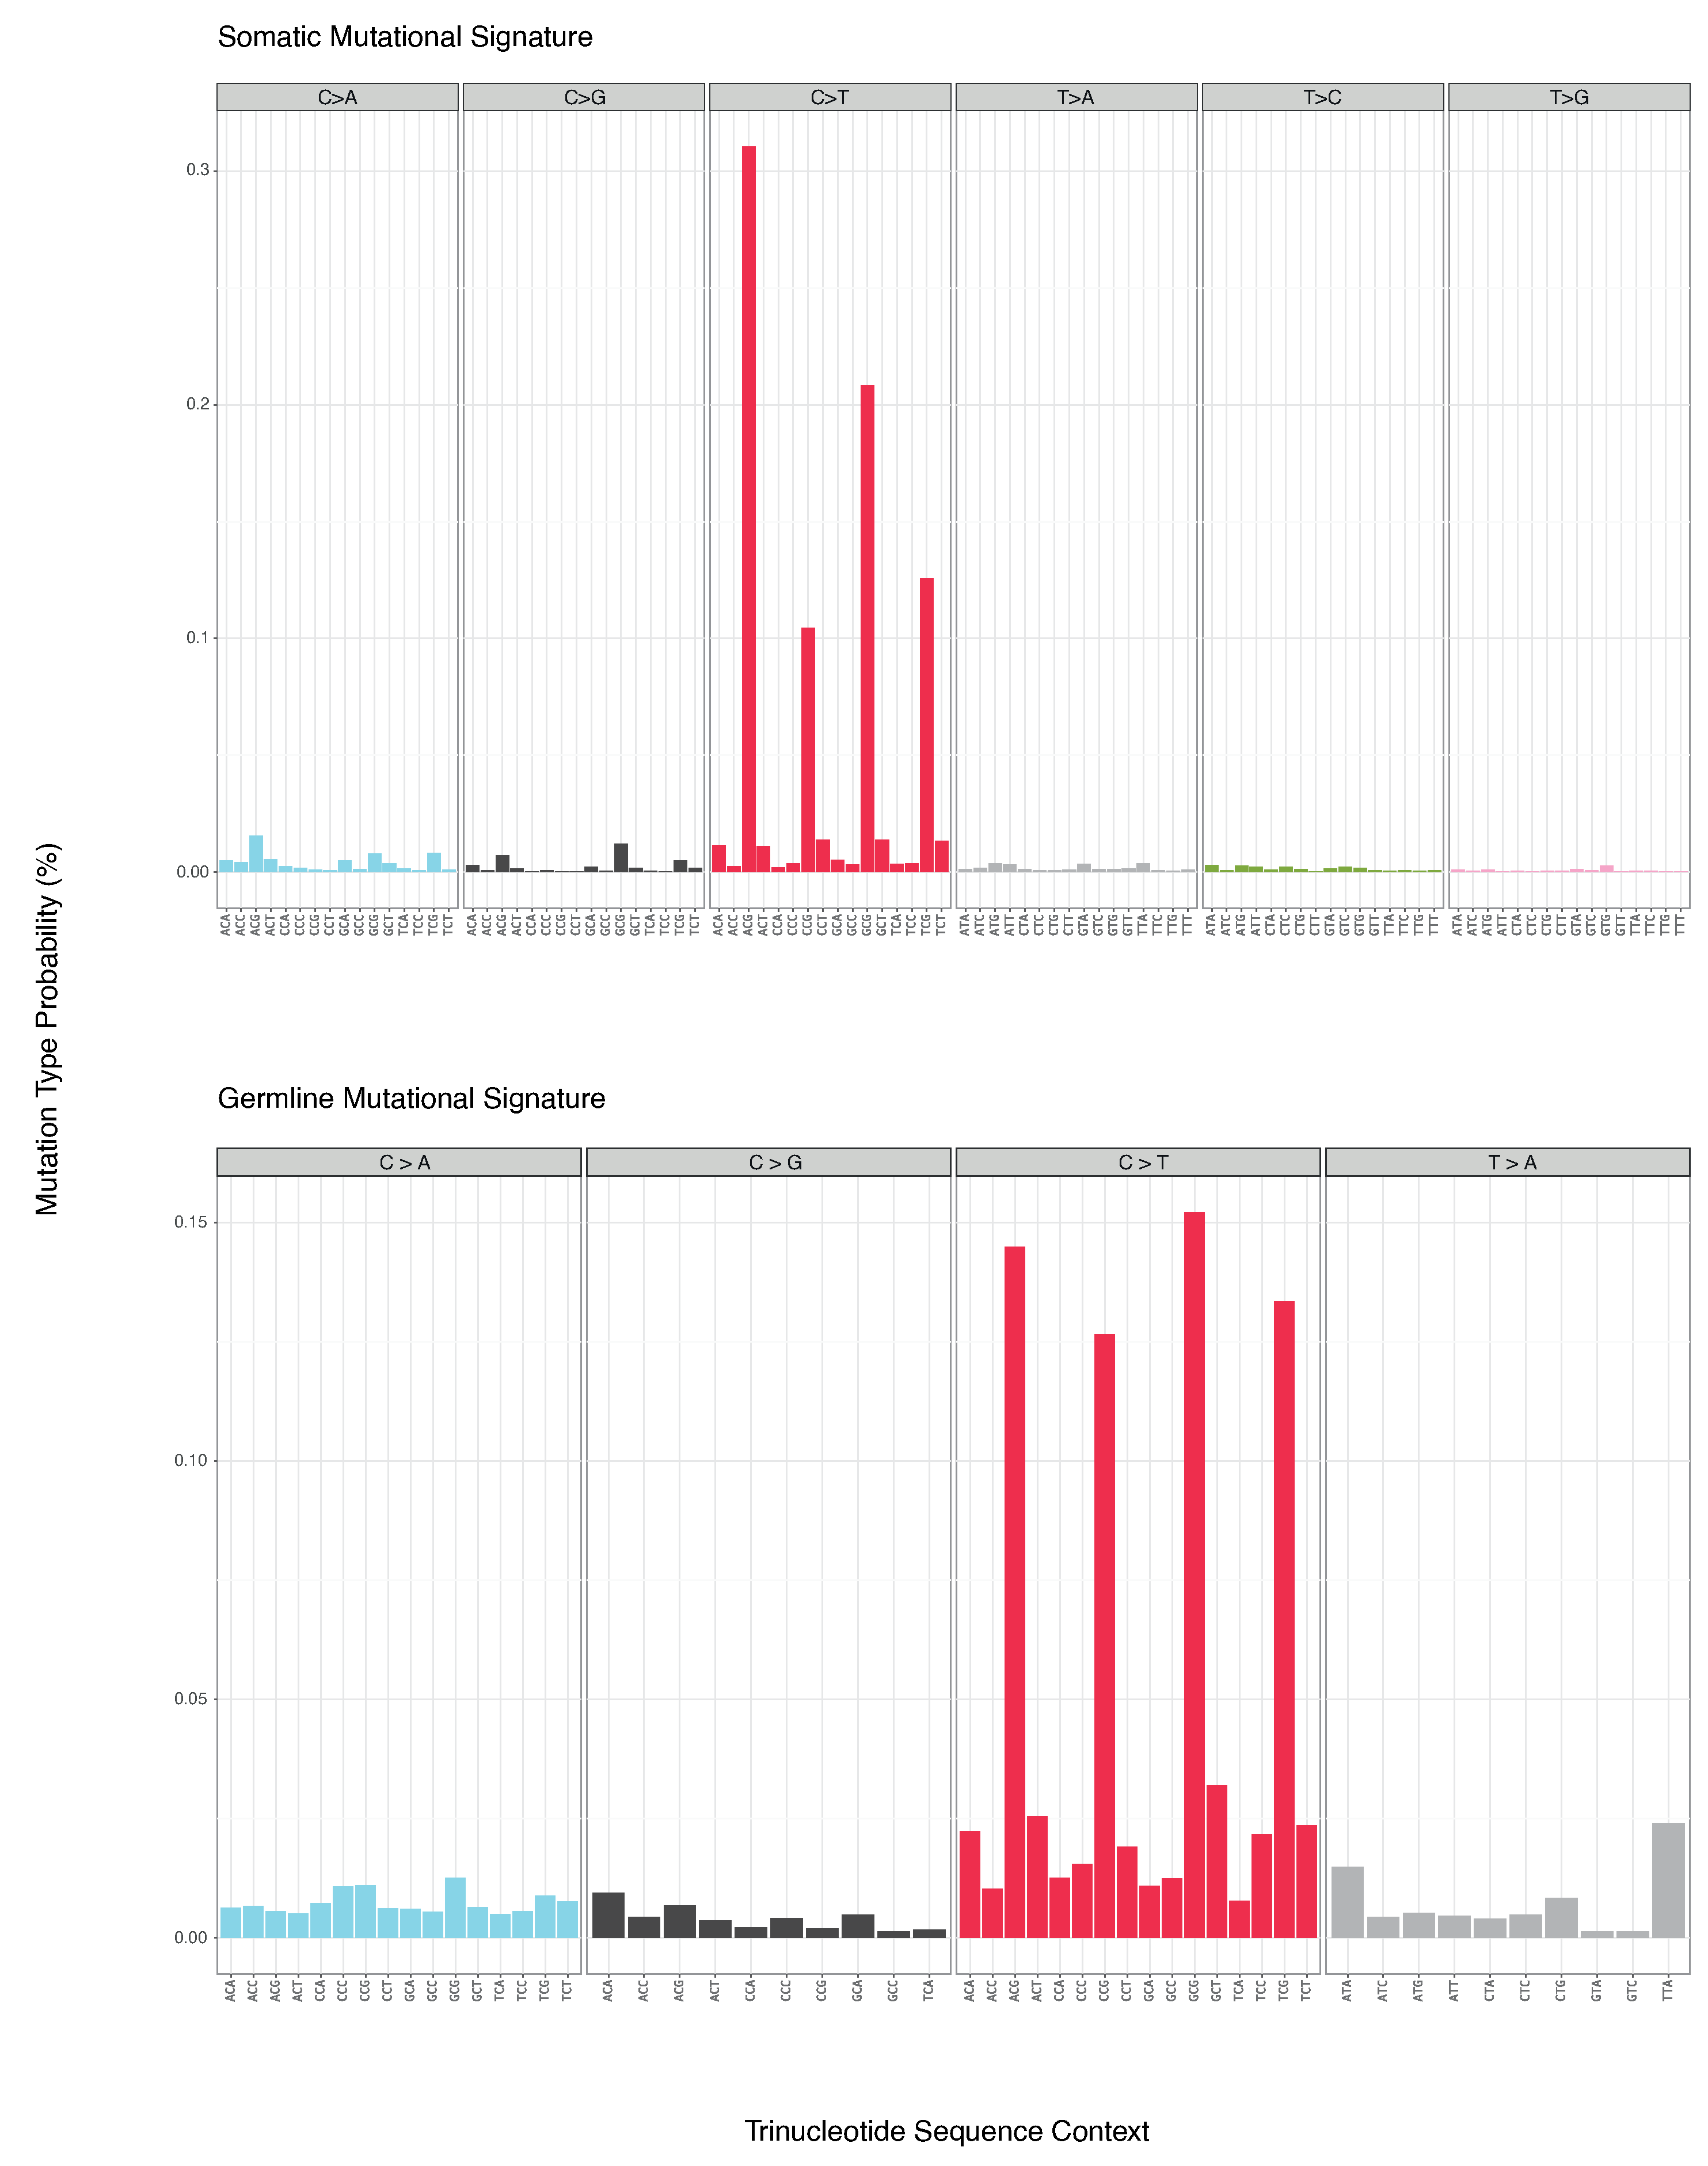
\includegraphics[width=1\textwidth]{Vector/TOL1_signature.pdf}}
\end{centering}
\end{figure}

\begin{figure}[htbp!]
\caption{TOL signature 2 (TOL2)}
\label{figure:TOL2}
\begin{centering}
\makebox[\textwidth][c]{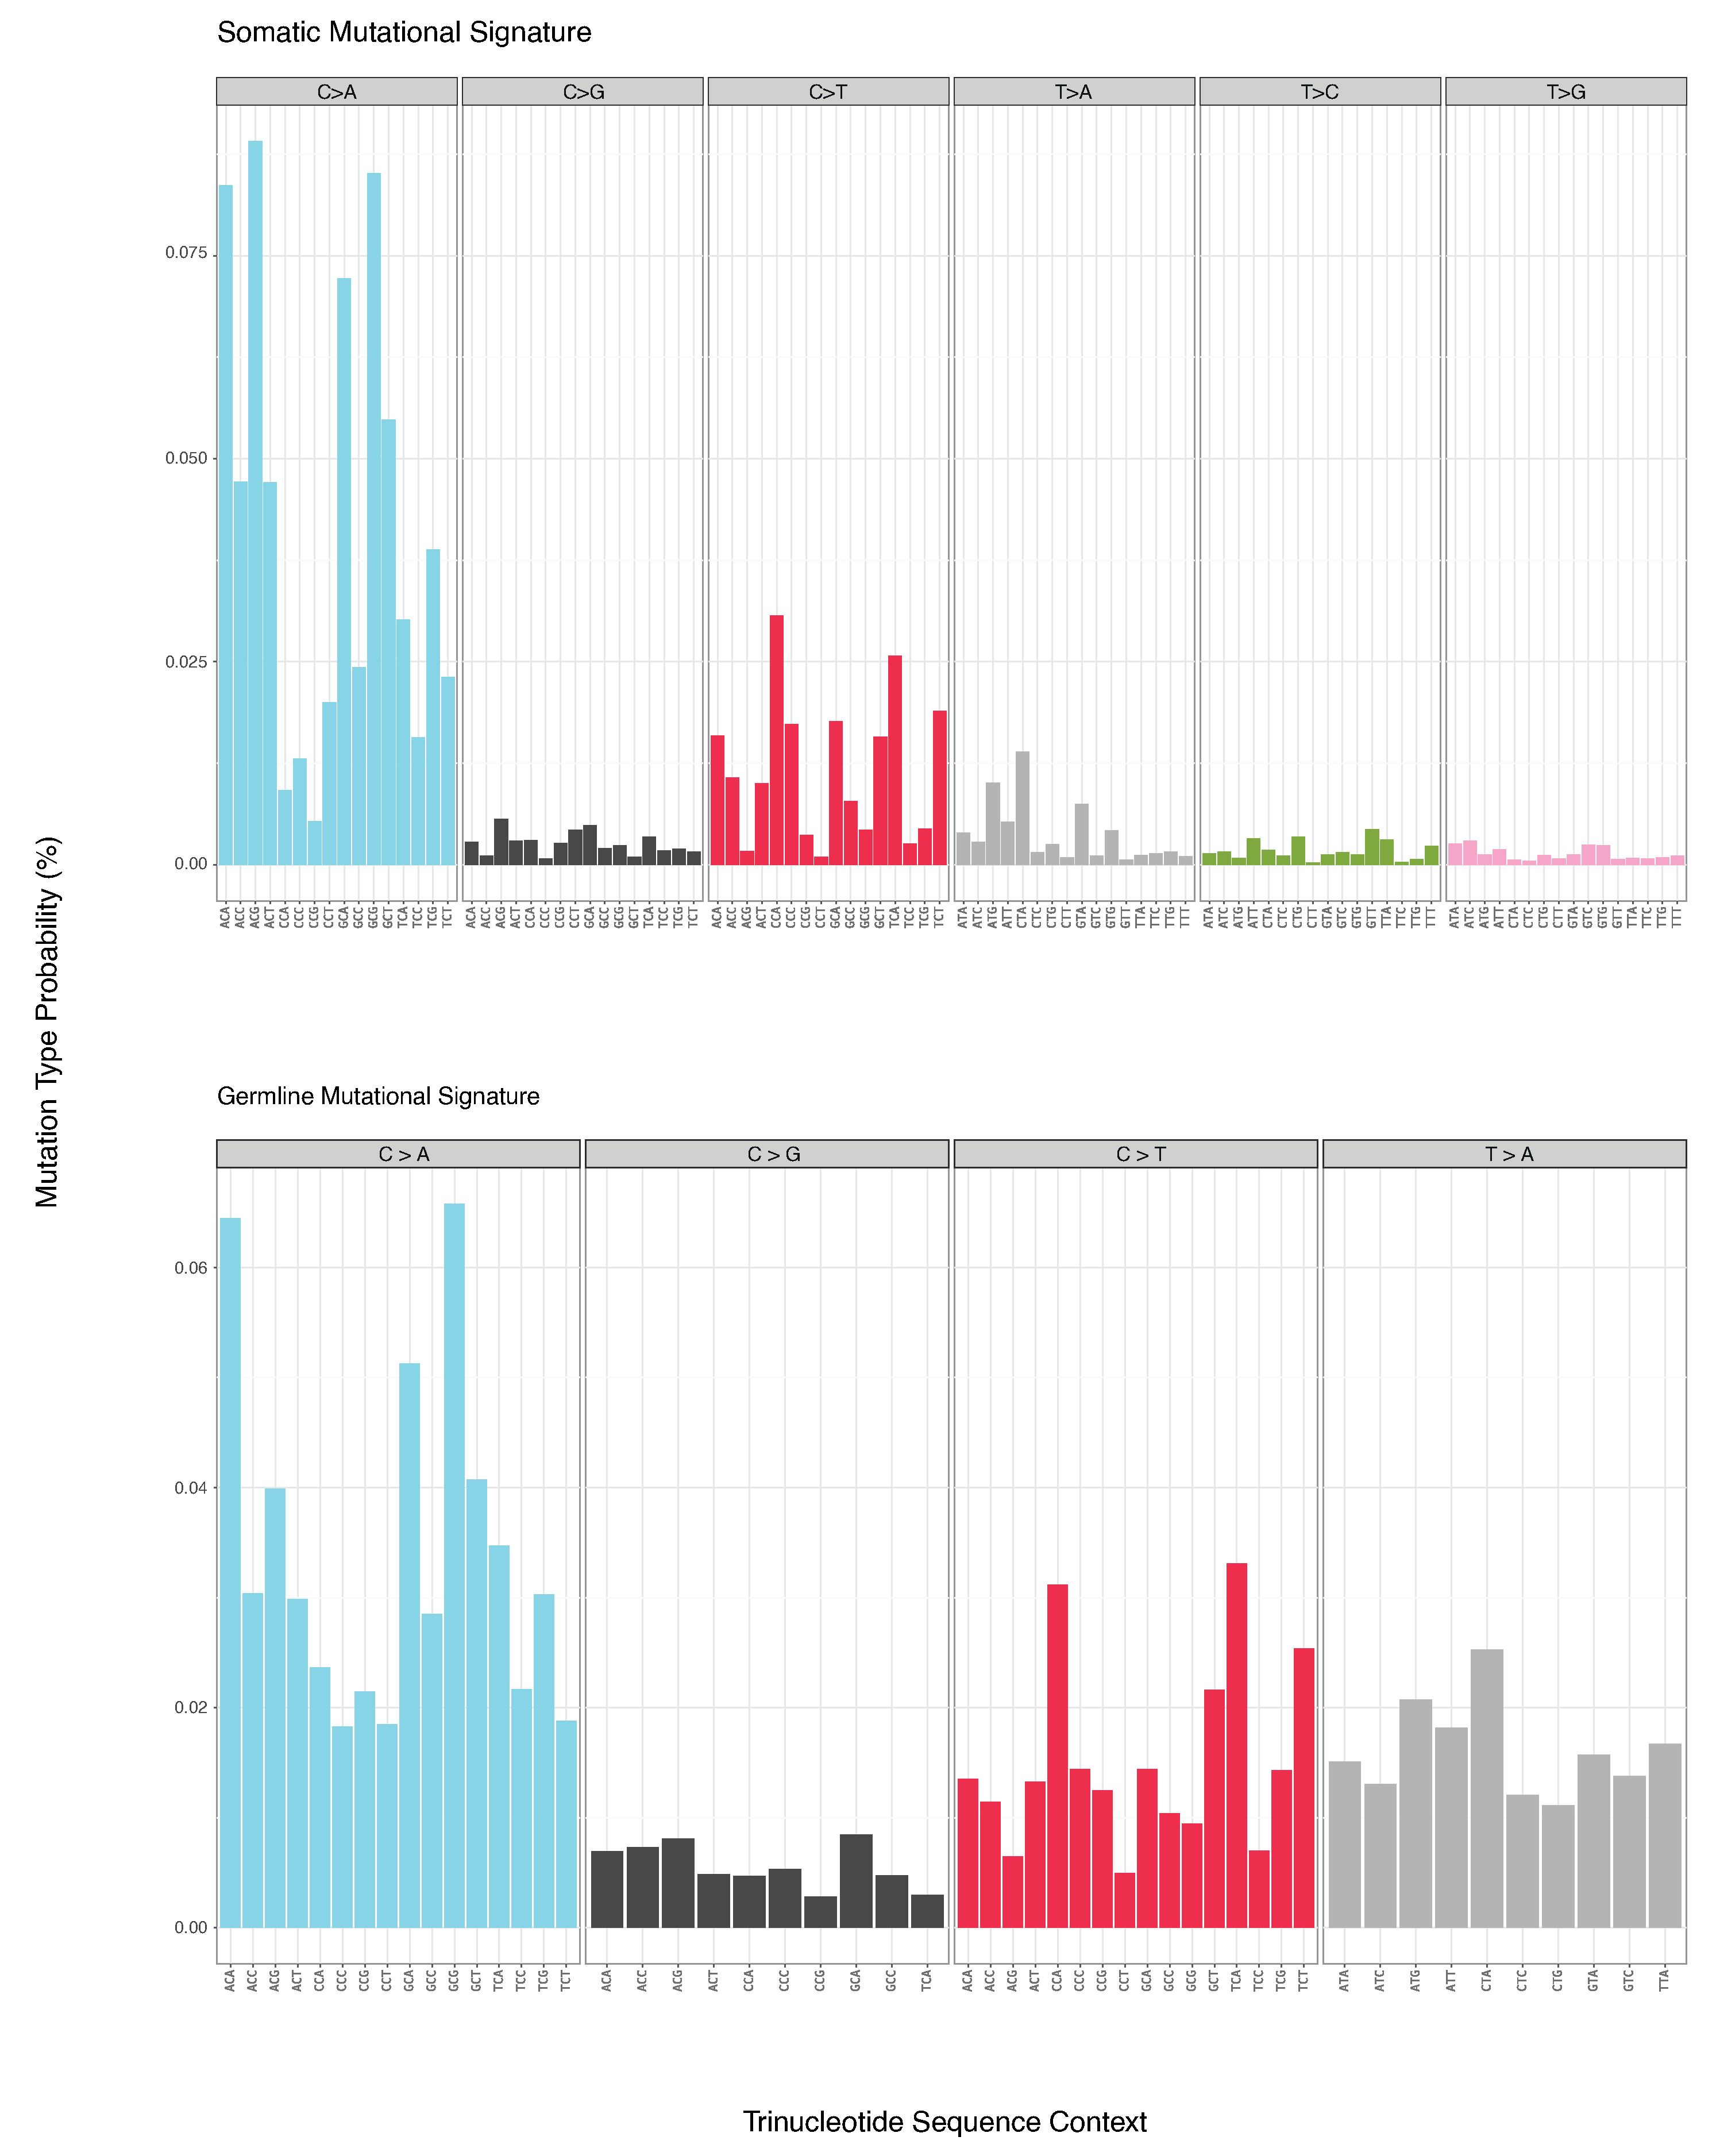
\includegraphics[width=1\textwidth]{Vector/TOL2_signature.pdf}}
\end{centering}
\end{figure}

\begin{figure}[htbp!]
\caption{TOL signature 3 (TOL3)}
\label{figure:TOL3}
\begin{centering}
\makebox[\textwidth][c]{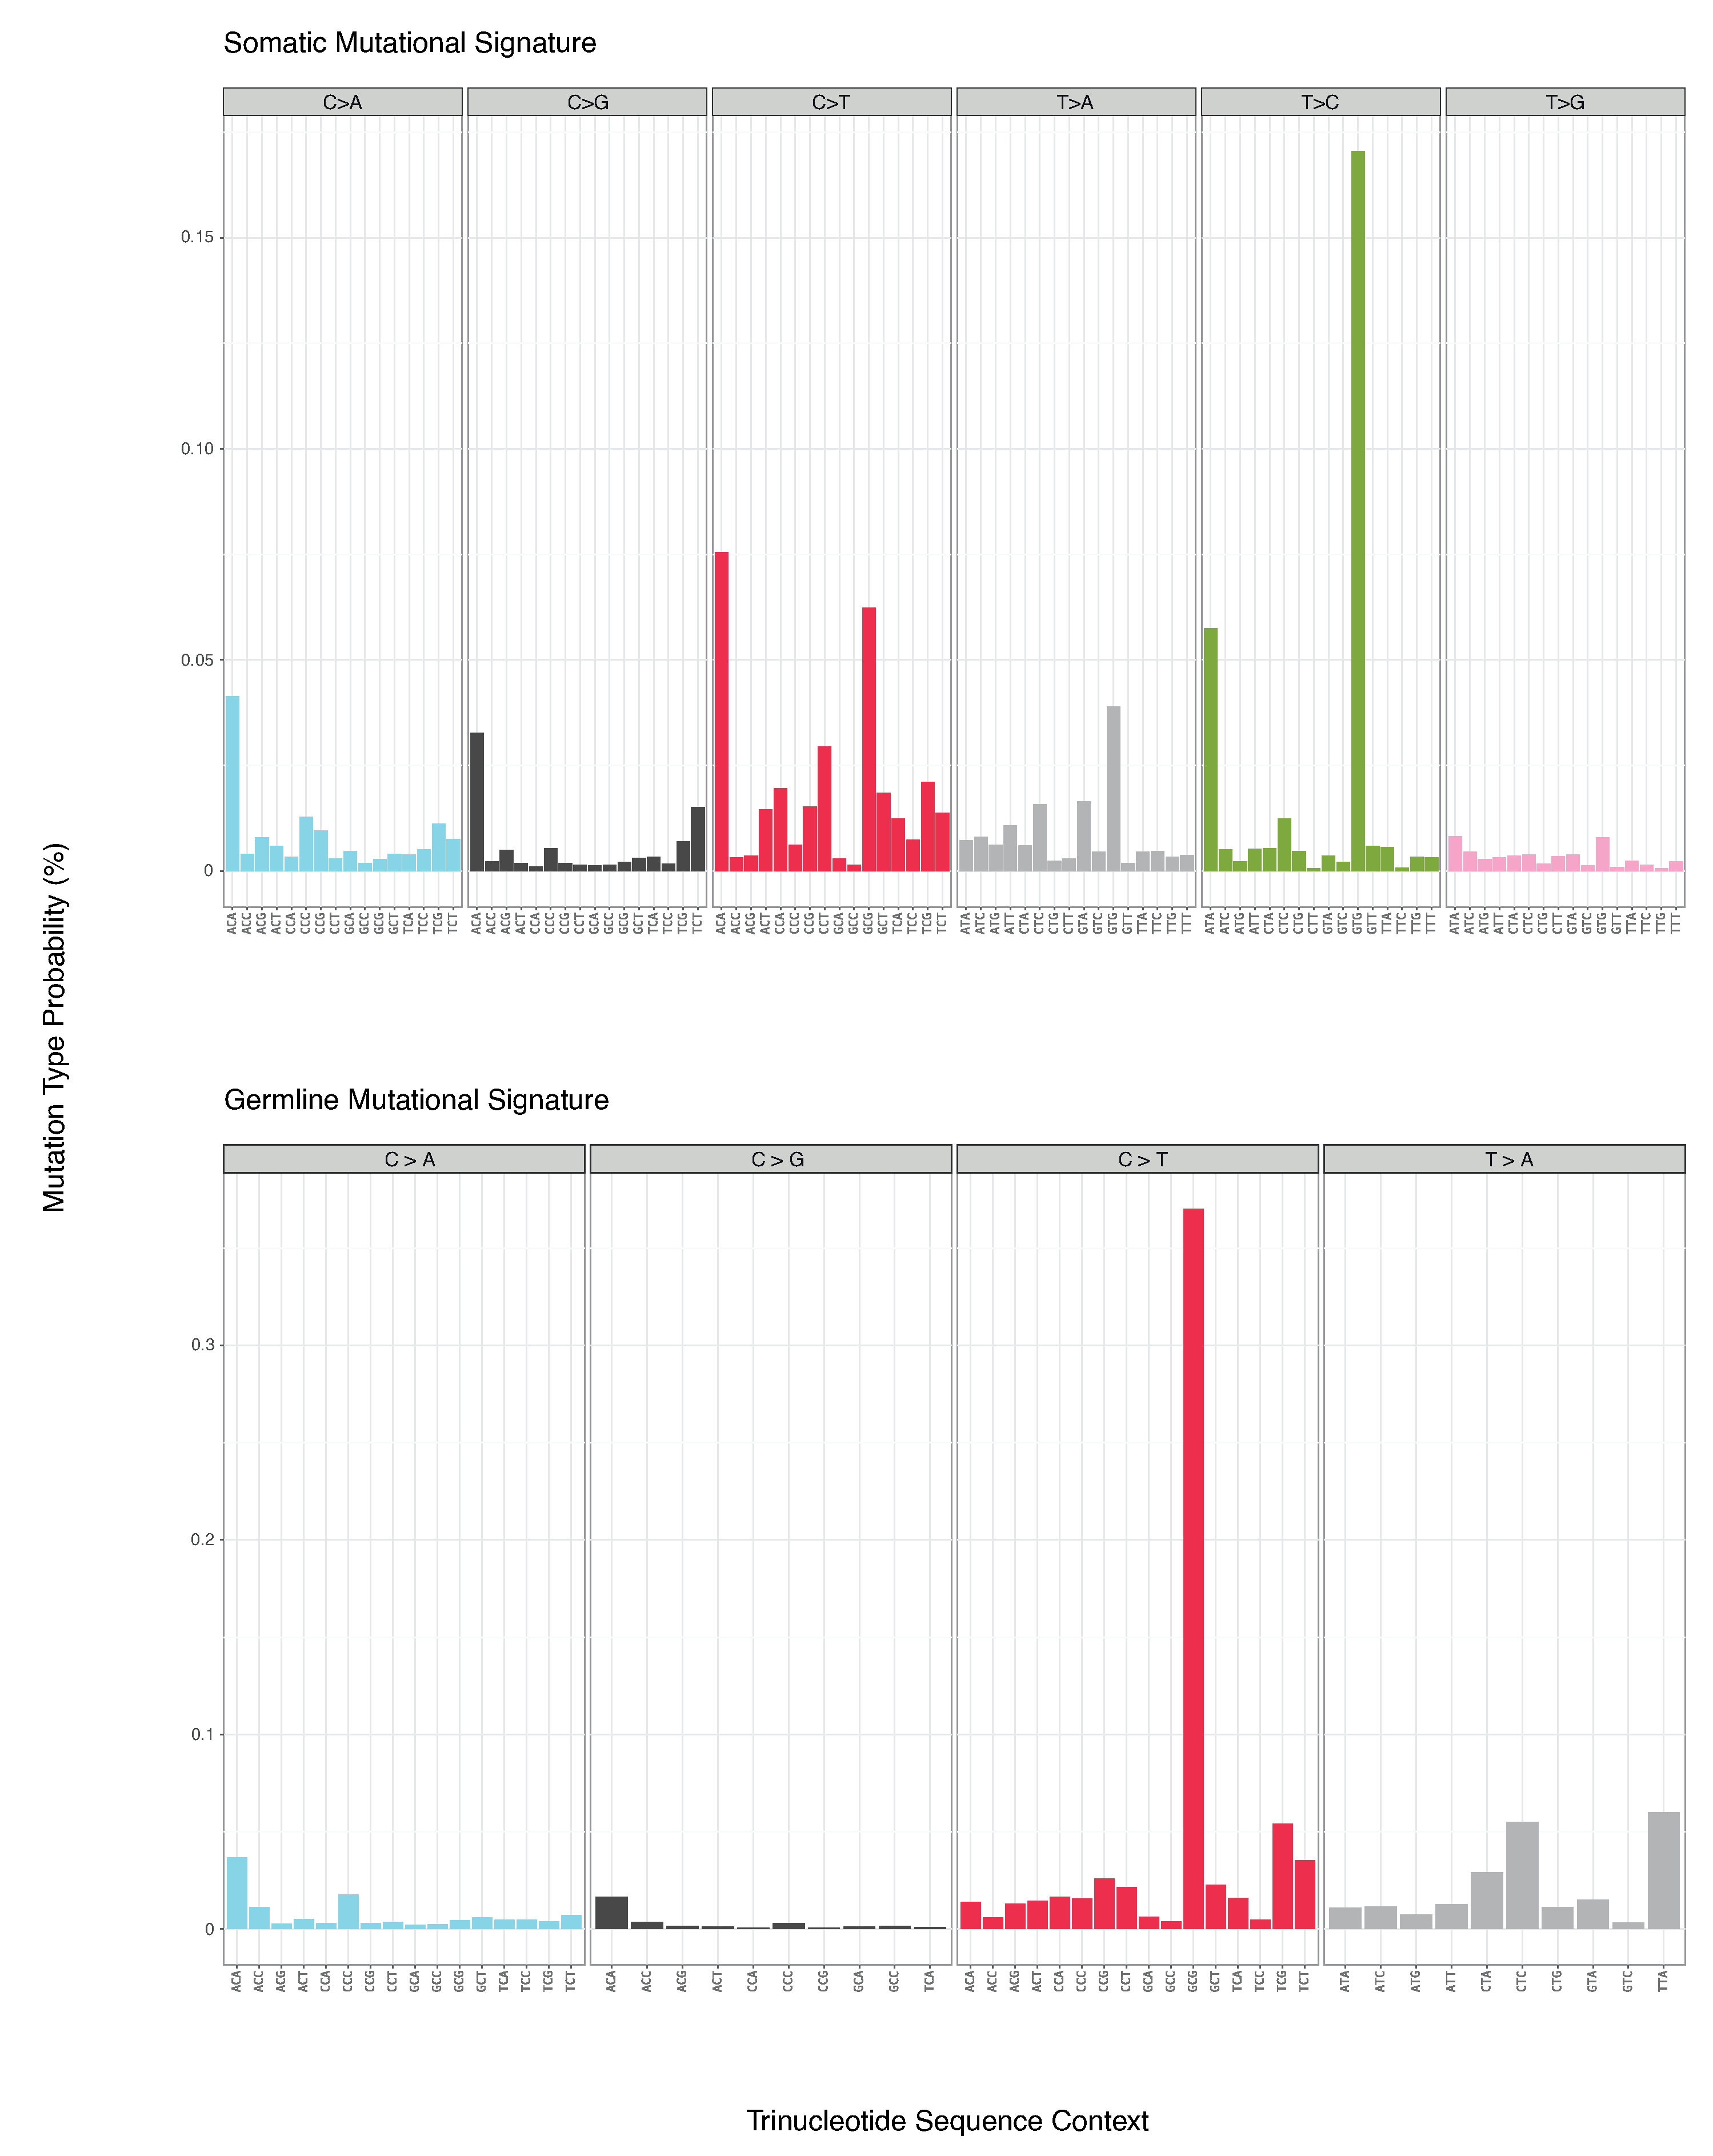
\includegraphics[width=1\textwidth]{Vector/TOL3_signature.pdf}}
\end{centering}
\end{figure}

\begin{figure}[htbp!]
\caption{TOL signature 4 (TOL4)}
\label{figure:TOL4}
\begin{centering}
\makebox[\textwidth][c]{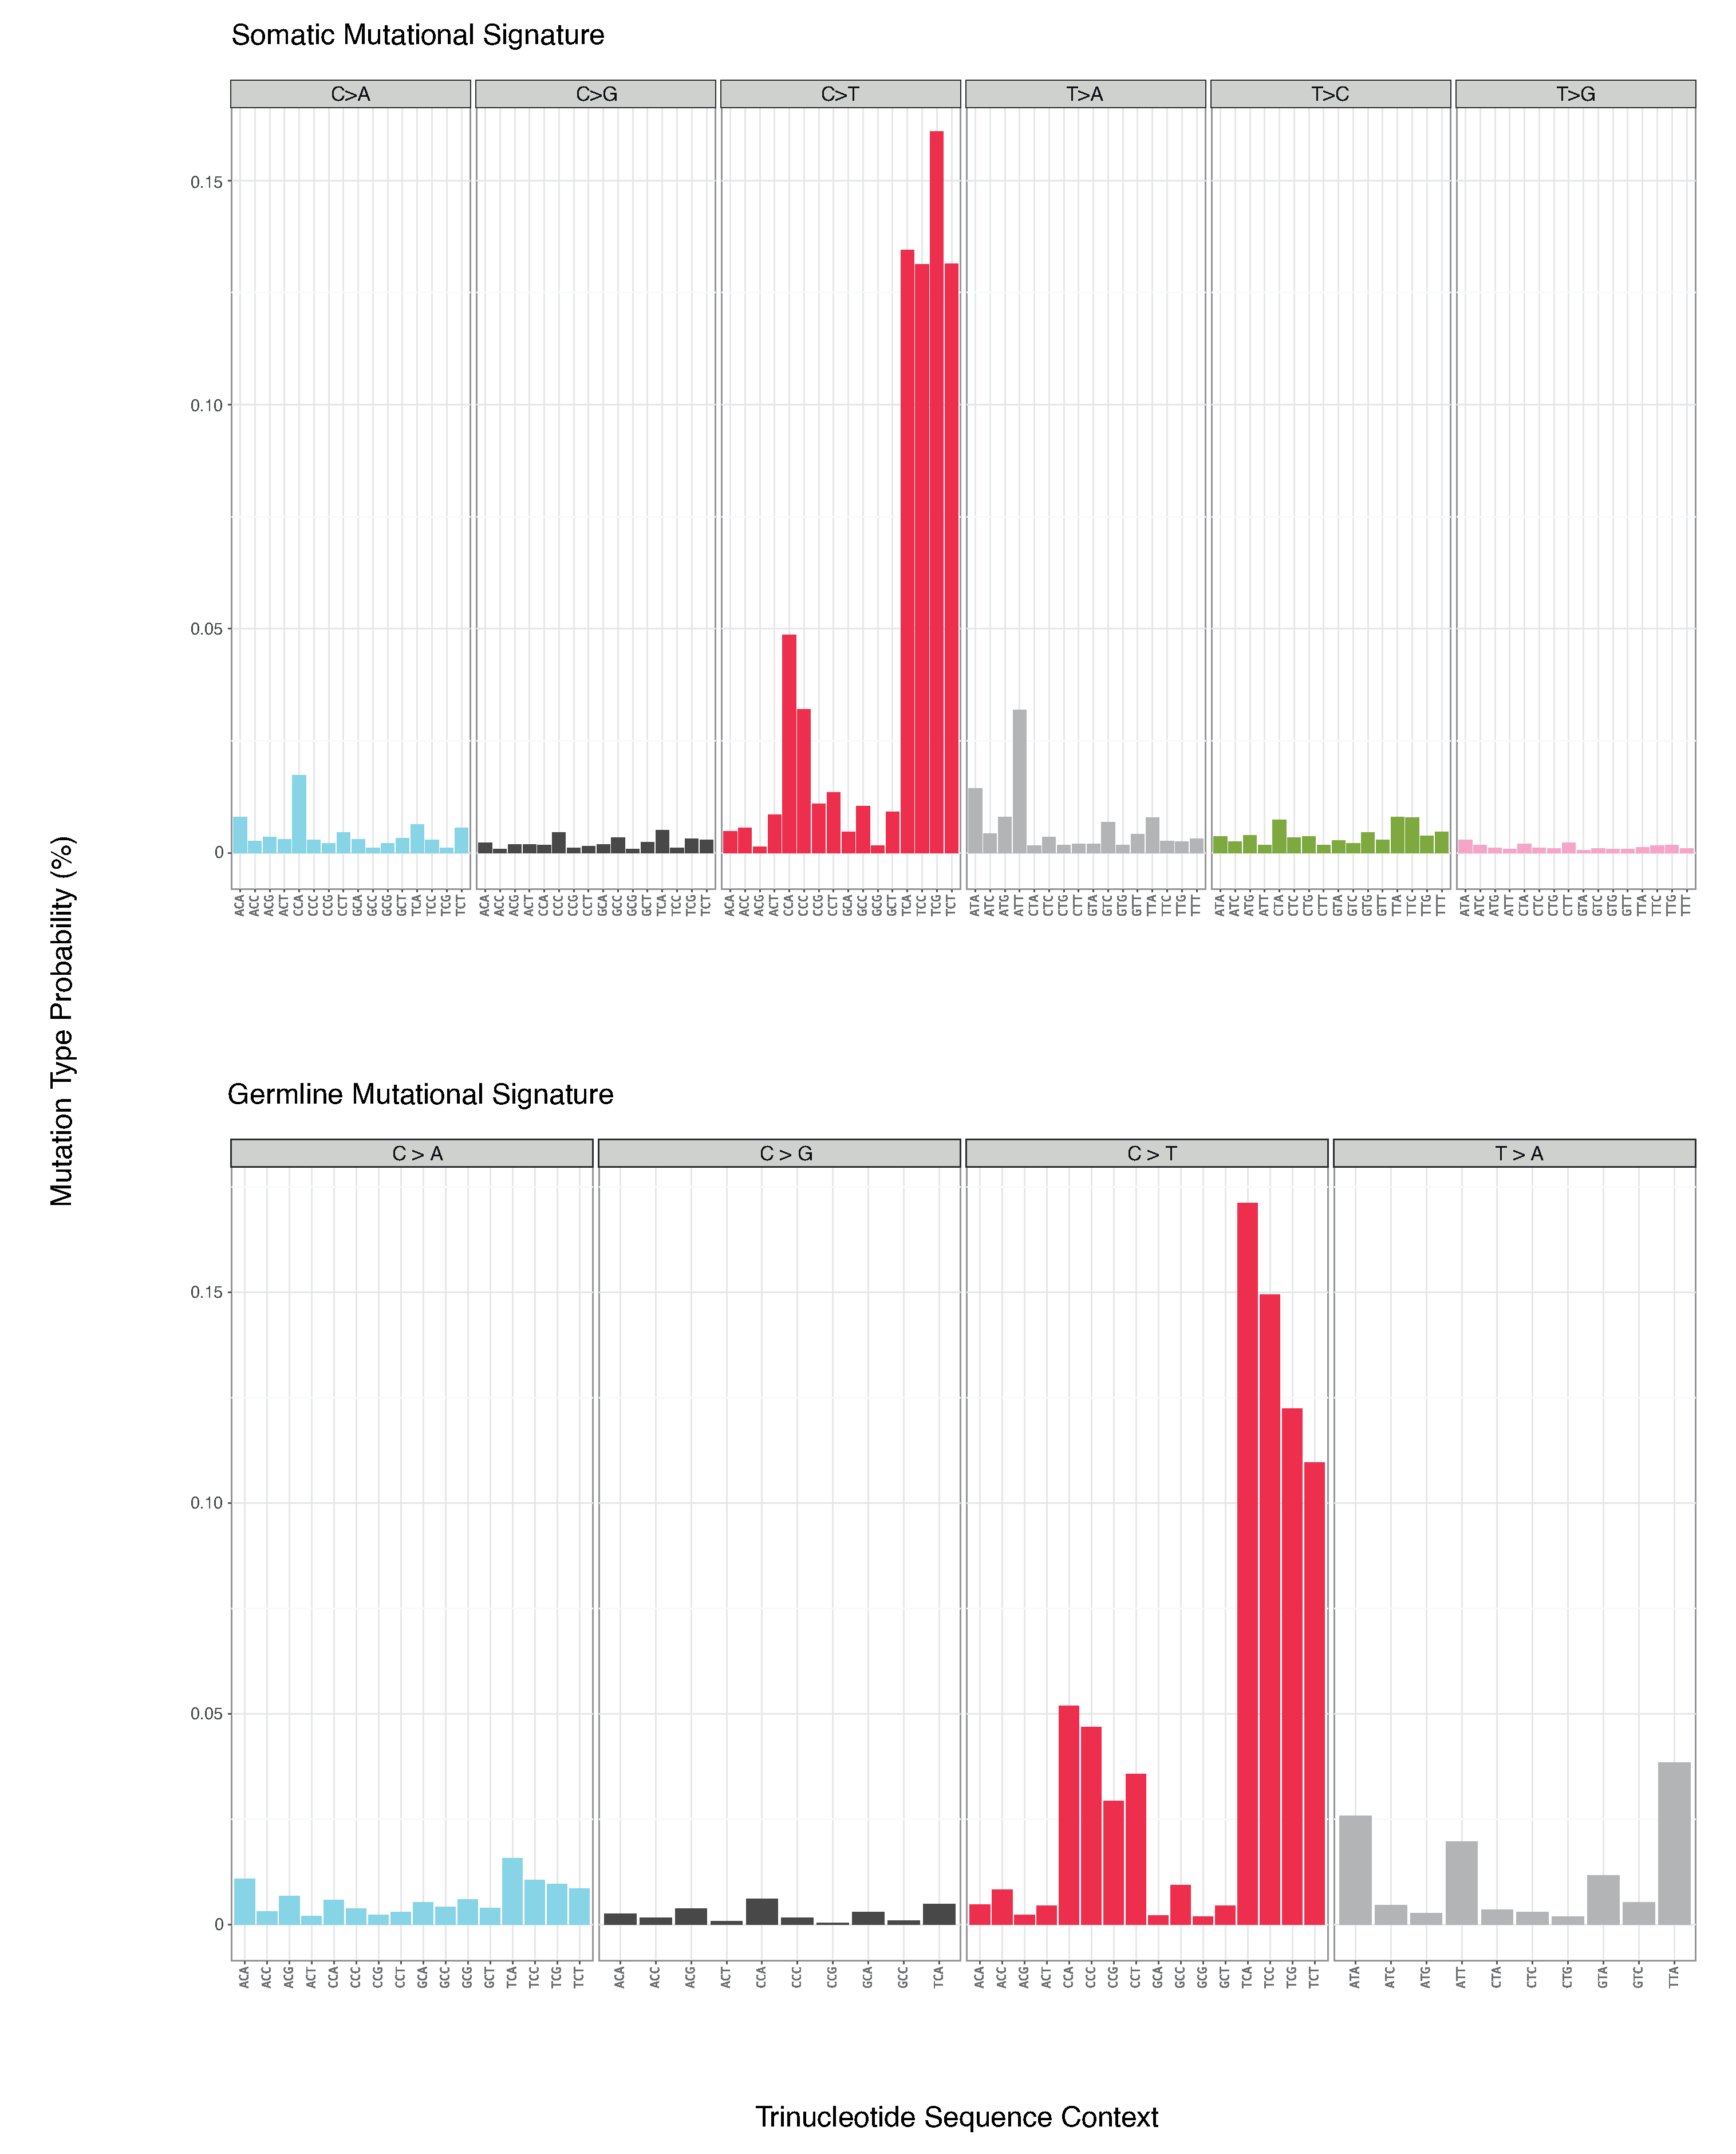
\includegraphics[width=1\textwidth]{Vector/TOL4_signature.pdf}}
\end{centering}
\end{figure}

\begin{figure}[htbp!]
\caption{TOL signature 5 (TOL5)}
\label{figure:TOL5}
\begin{centering}
\makebox[\textwidth][c]{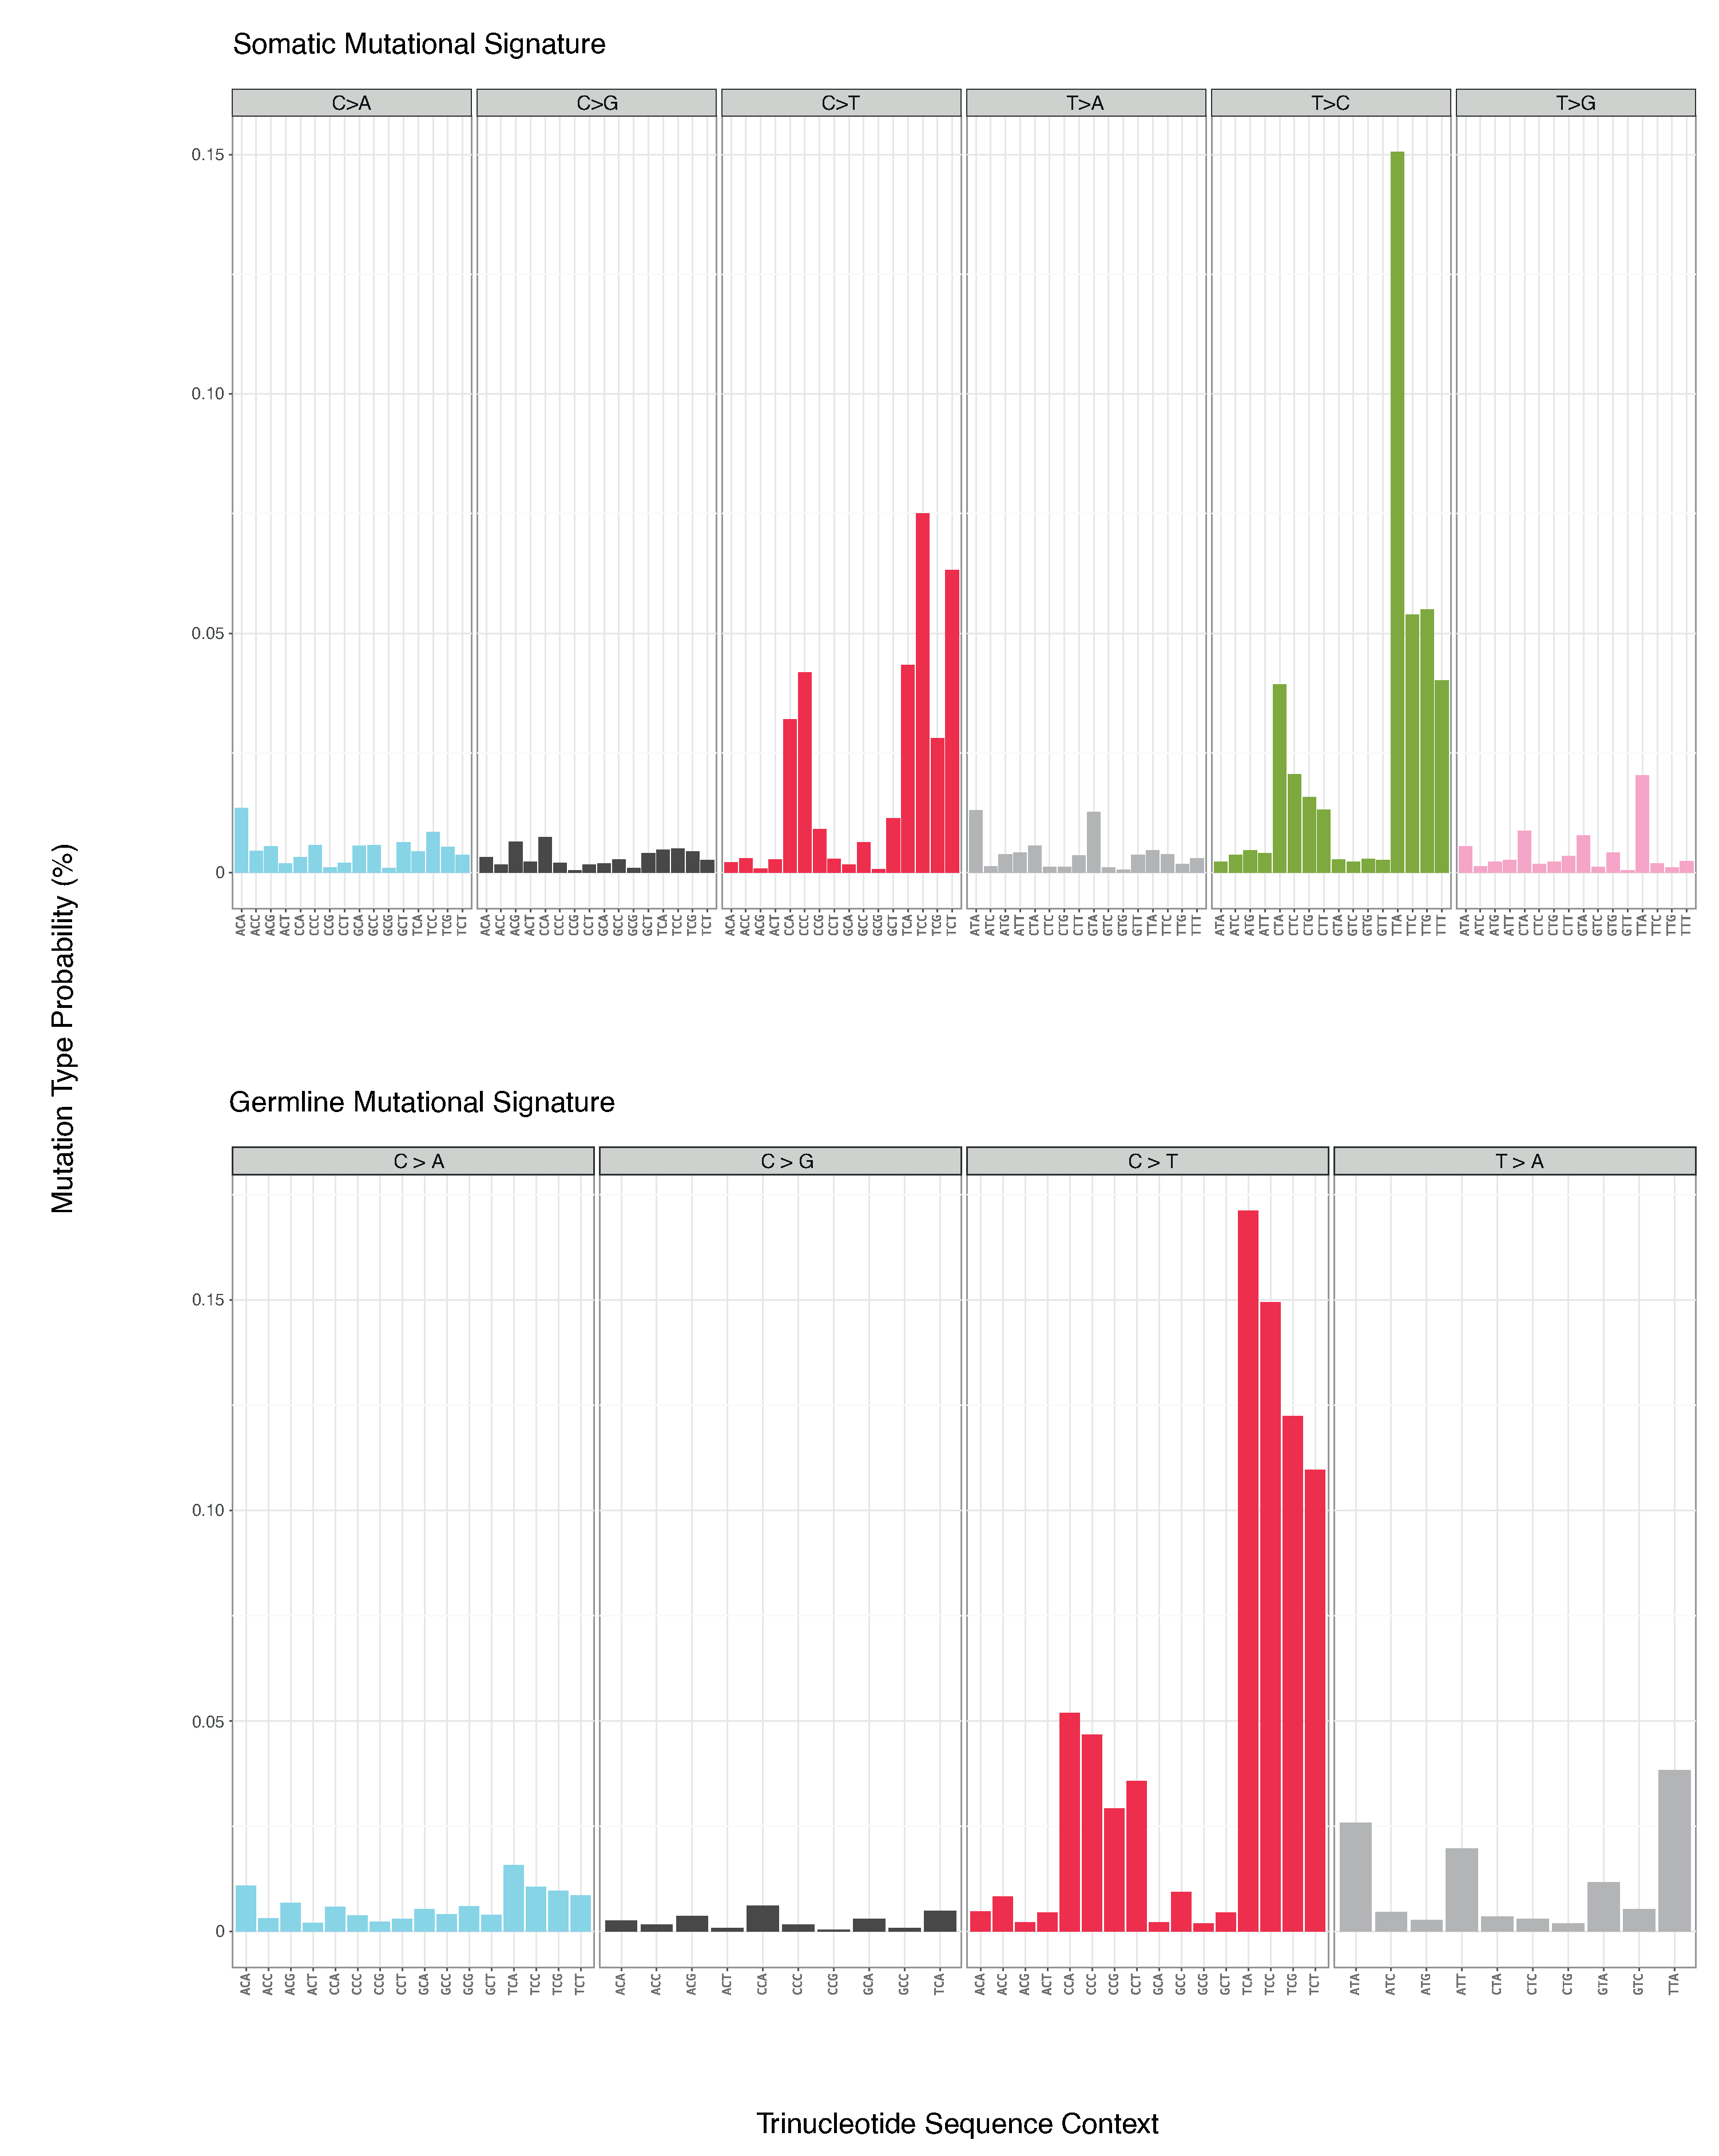
\includegraphics[width=1\textwidth]{Vector/TOL5_signature.pdf}}
\end{centering}
\end{figure}

\begin{figure}[htbp!]
\caption{SBS96 and SBS192 somatic mutational spectra in \textit{Athalia rosae} (coleseed sawfly)}
\label{figure:iyAthRosa1-SBS96-SBS192}
\begin{centering}
\makebox[\textwidth][c]{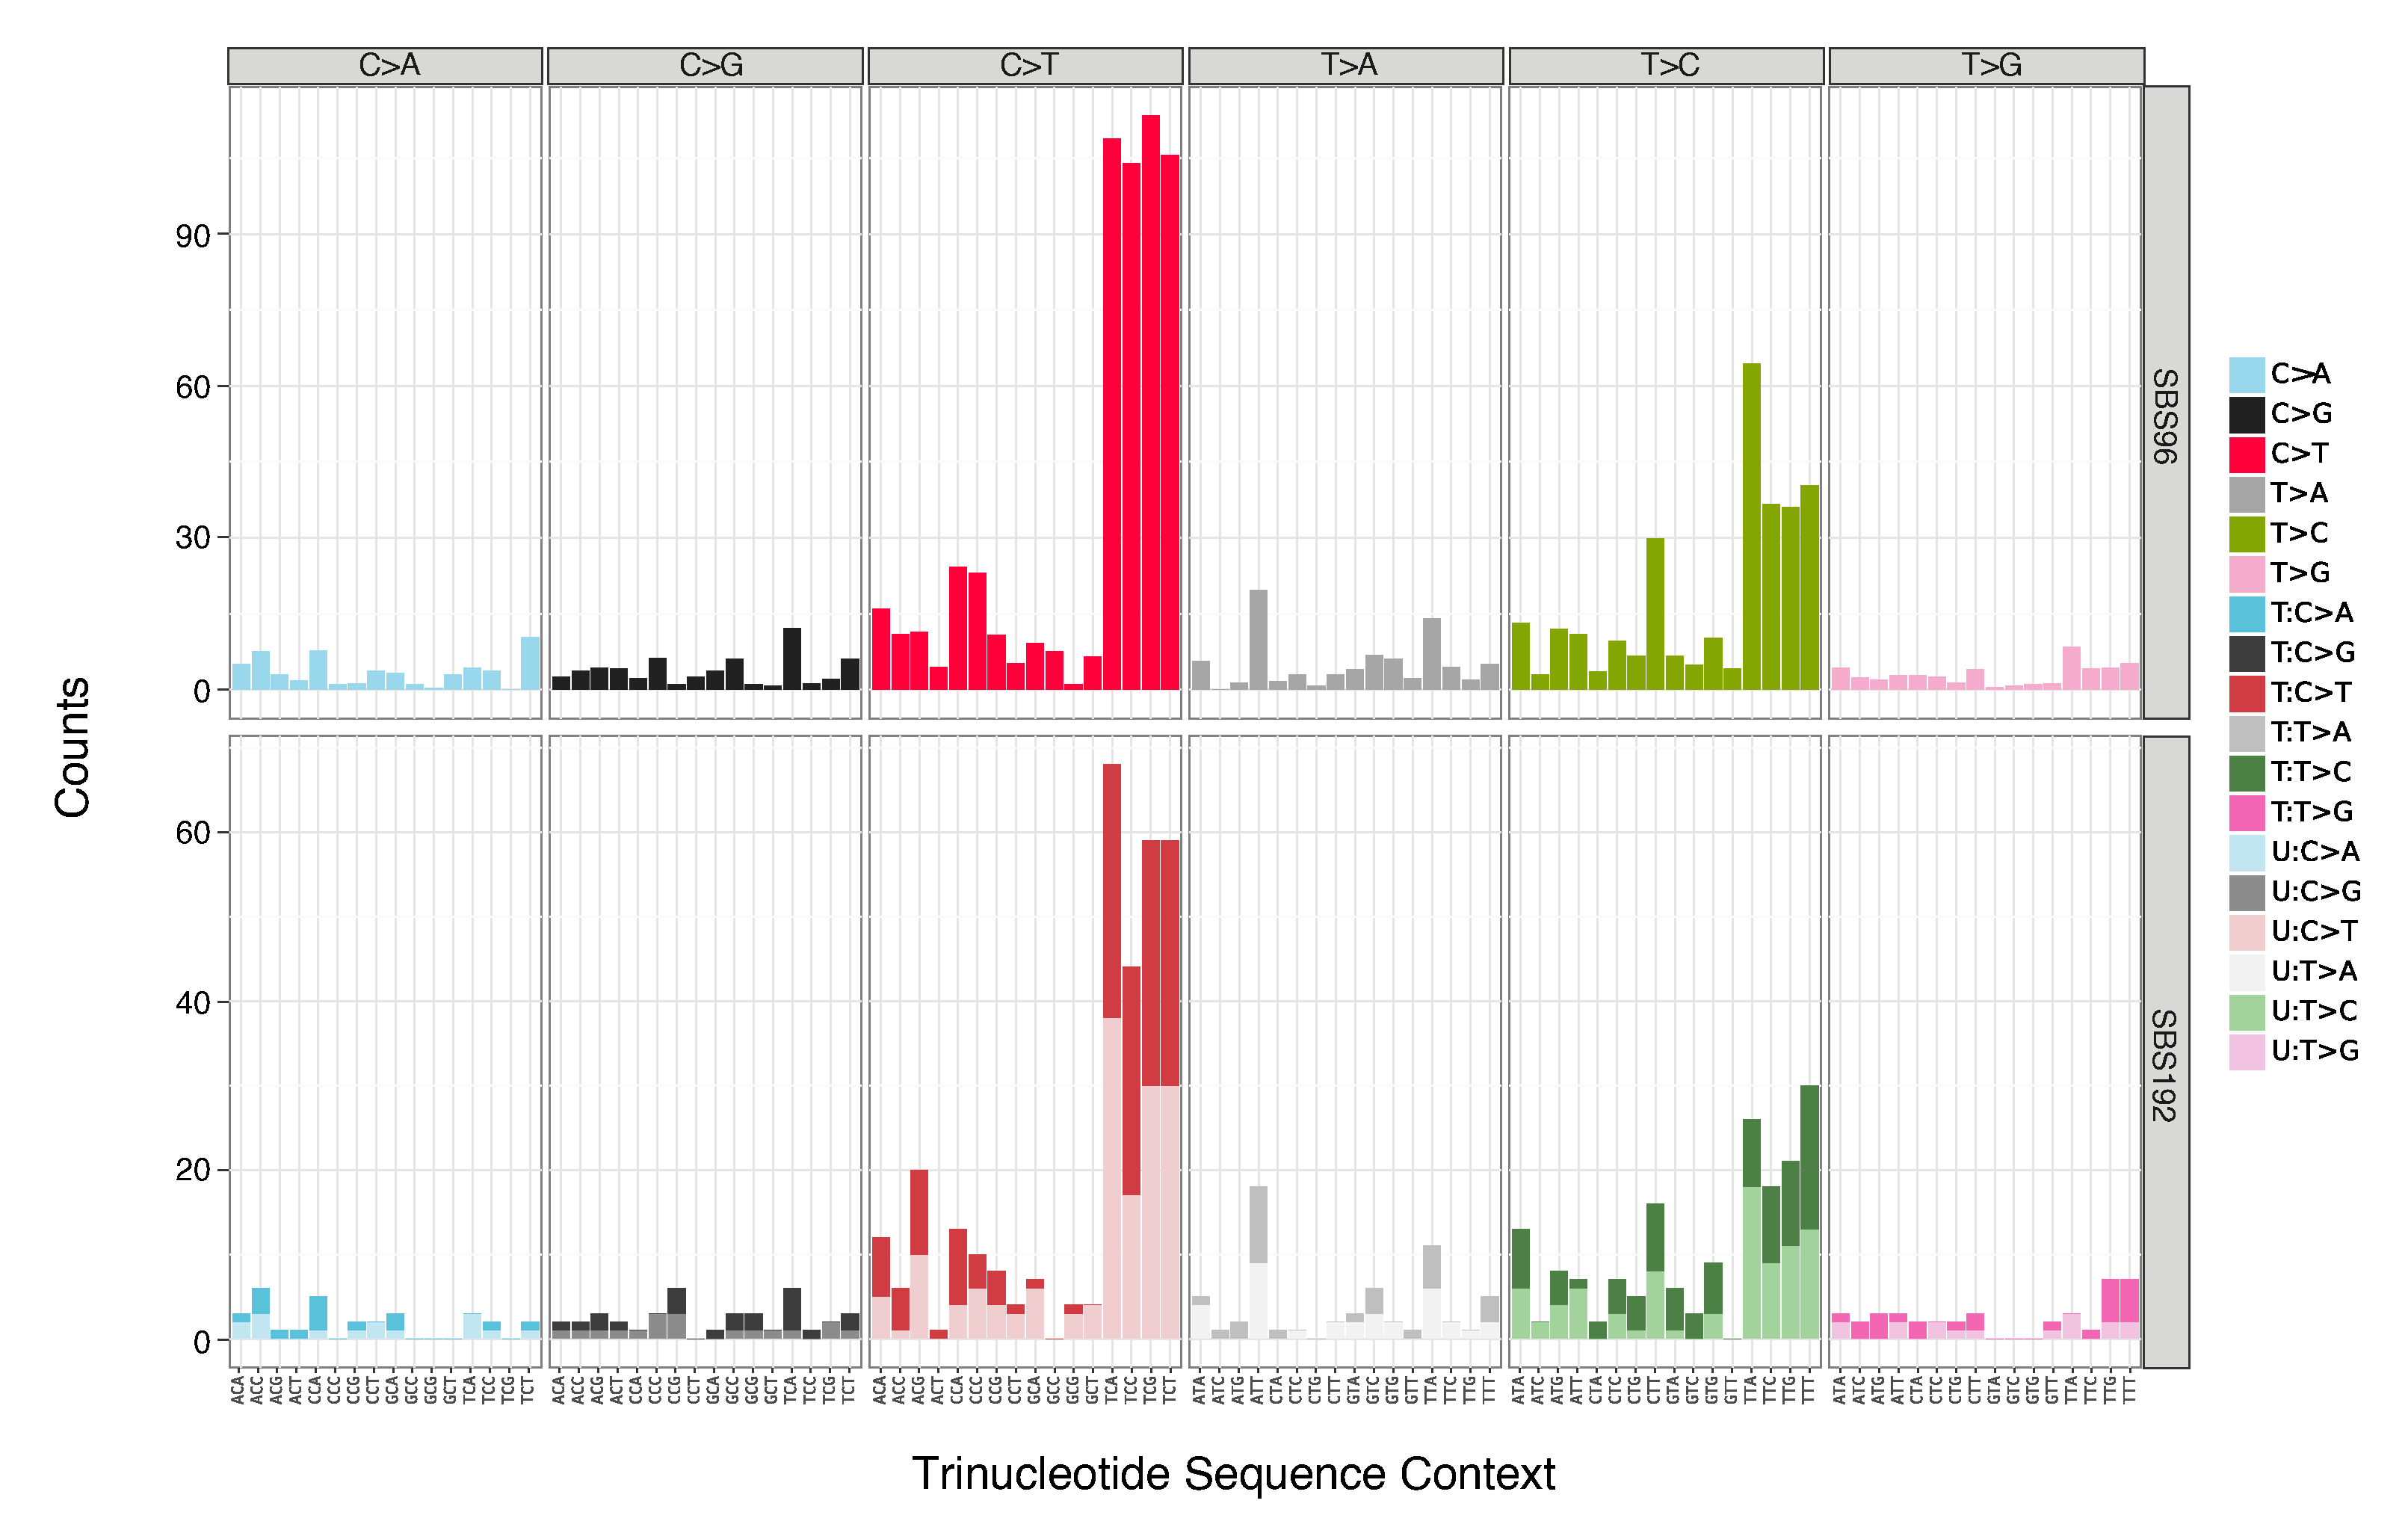
\includegraphics[width=1\textwidth]{Vector/iyAthRosa1.somatic_sbs96_sbs192.pdf}}
\end{centering}
\floatfoot{T stands for transcribed and U stands for untranscribed. Inter-genic somatic mutations are excluded from SBS192 somatic mutational spectra.}
\end{figure}

\begin{figure}[htbp!]
\caption{TOL signature 5 (TOL5) transformation and comparison}
\label{figure:TOL5-somatic-germline}
\begin{centering}
\makebox[\textwidth][c]{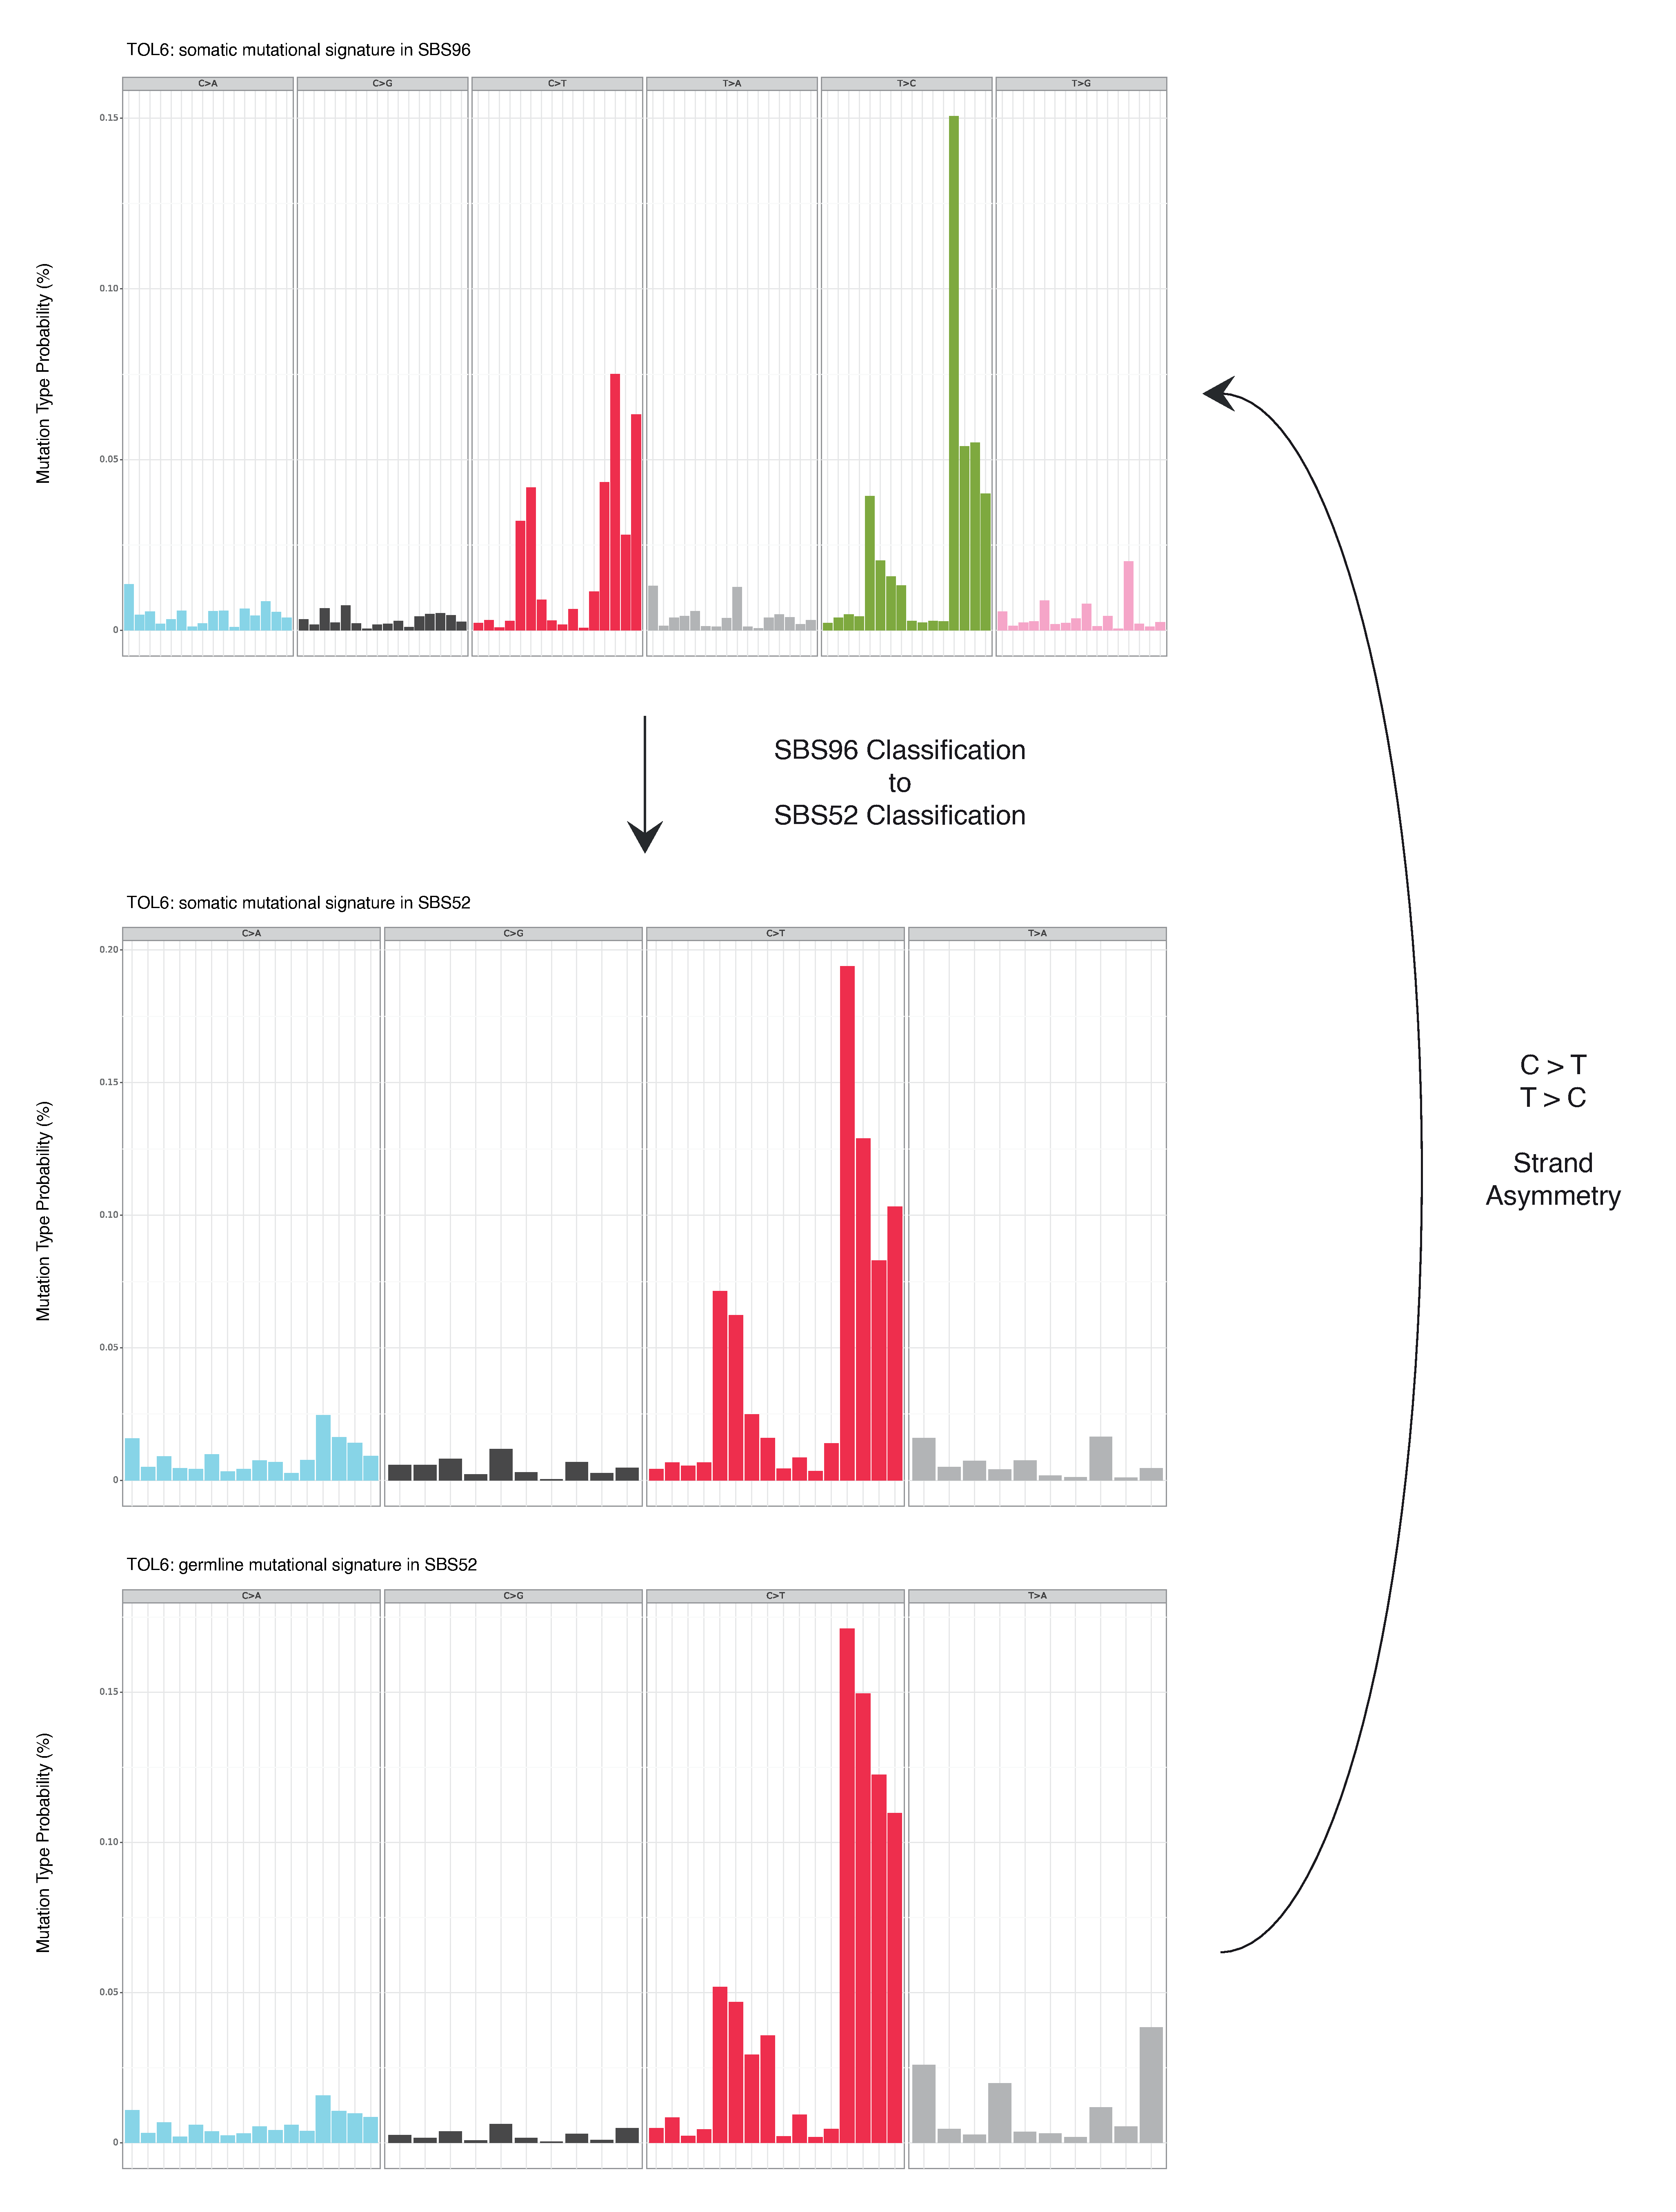
\includegraphics[width=0.9\textwidth]{Vector/TOL5_somatic_germline_signature_SBS96_to_SBS52.pdf}}
\end{centering}
\end{figure}

\begin{figure}[htbp!]
\caption{TOL signature 6 (TOL6)}
\label{figure:TOL6}
\begin{centering}
\makebox[\textwidth][c]{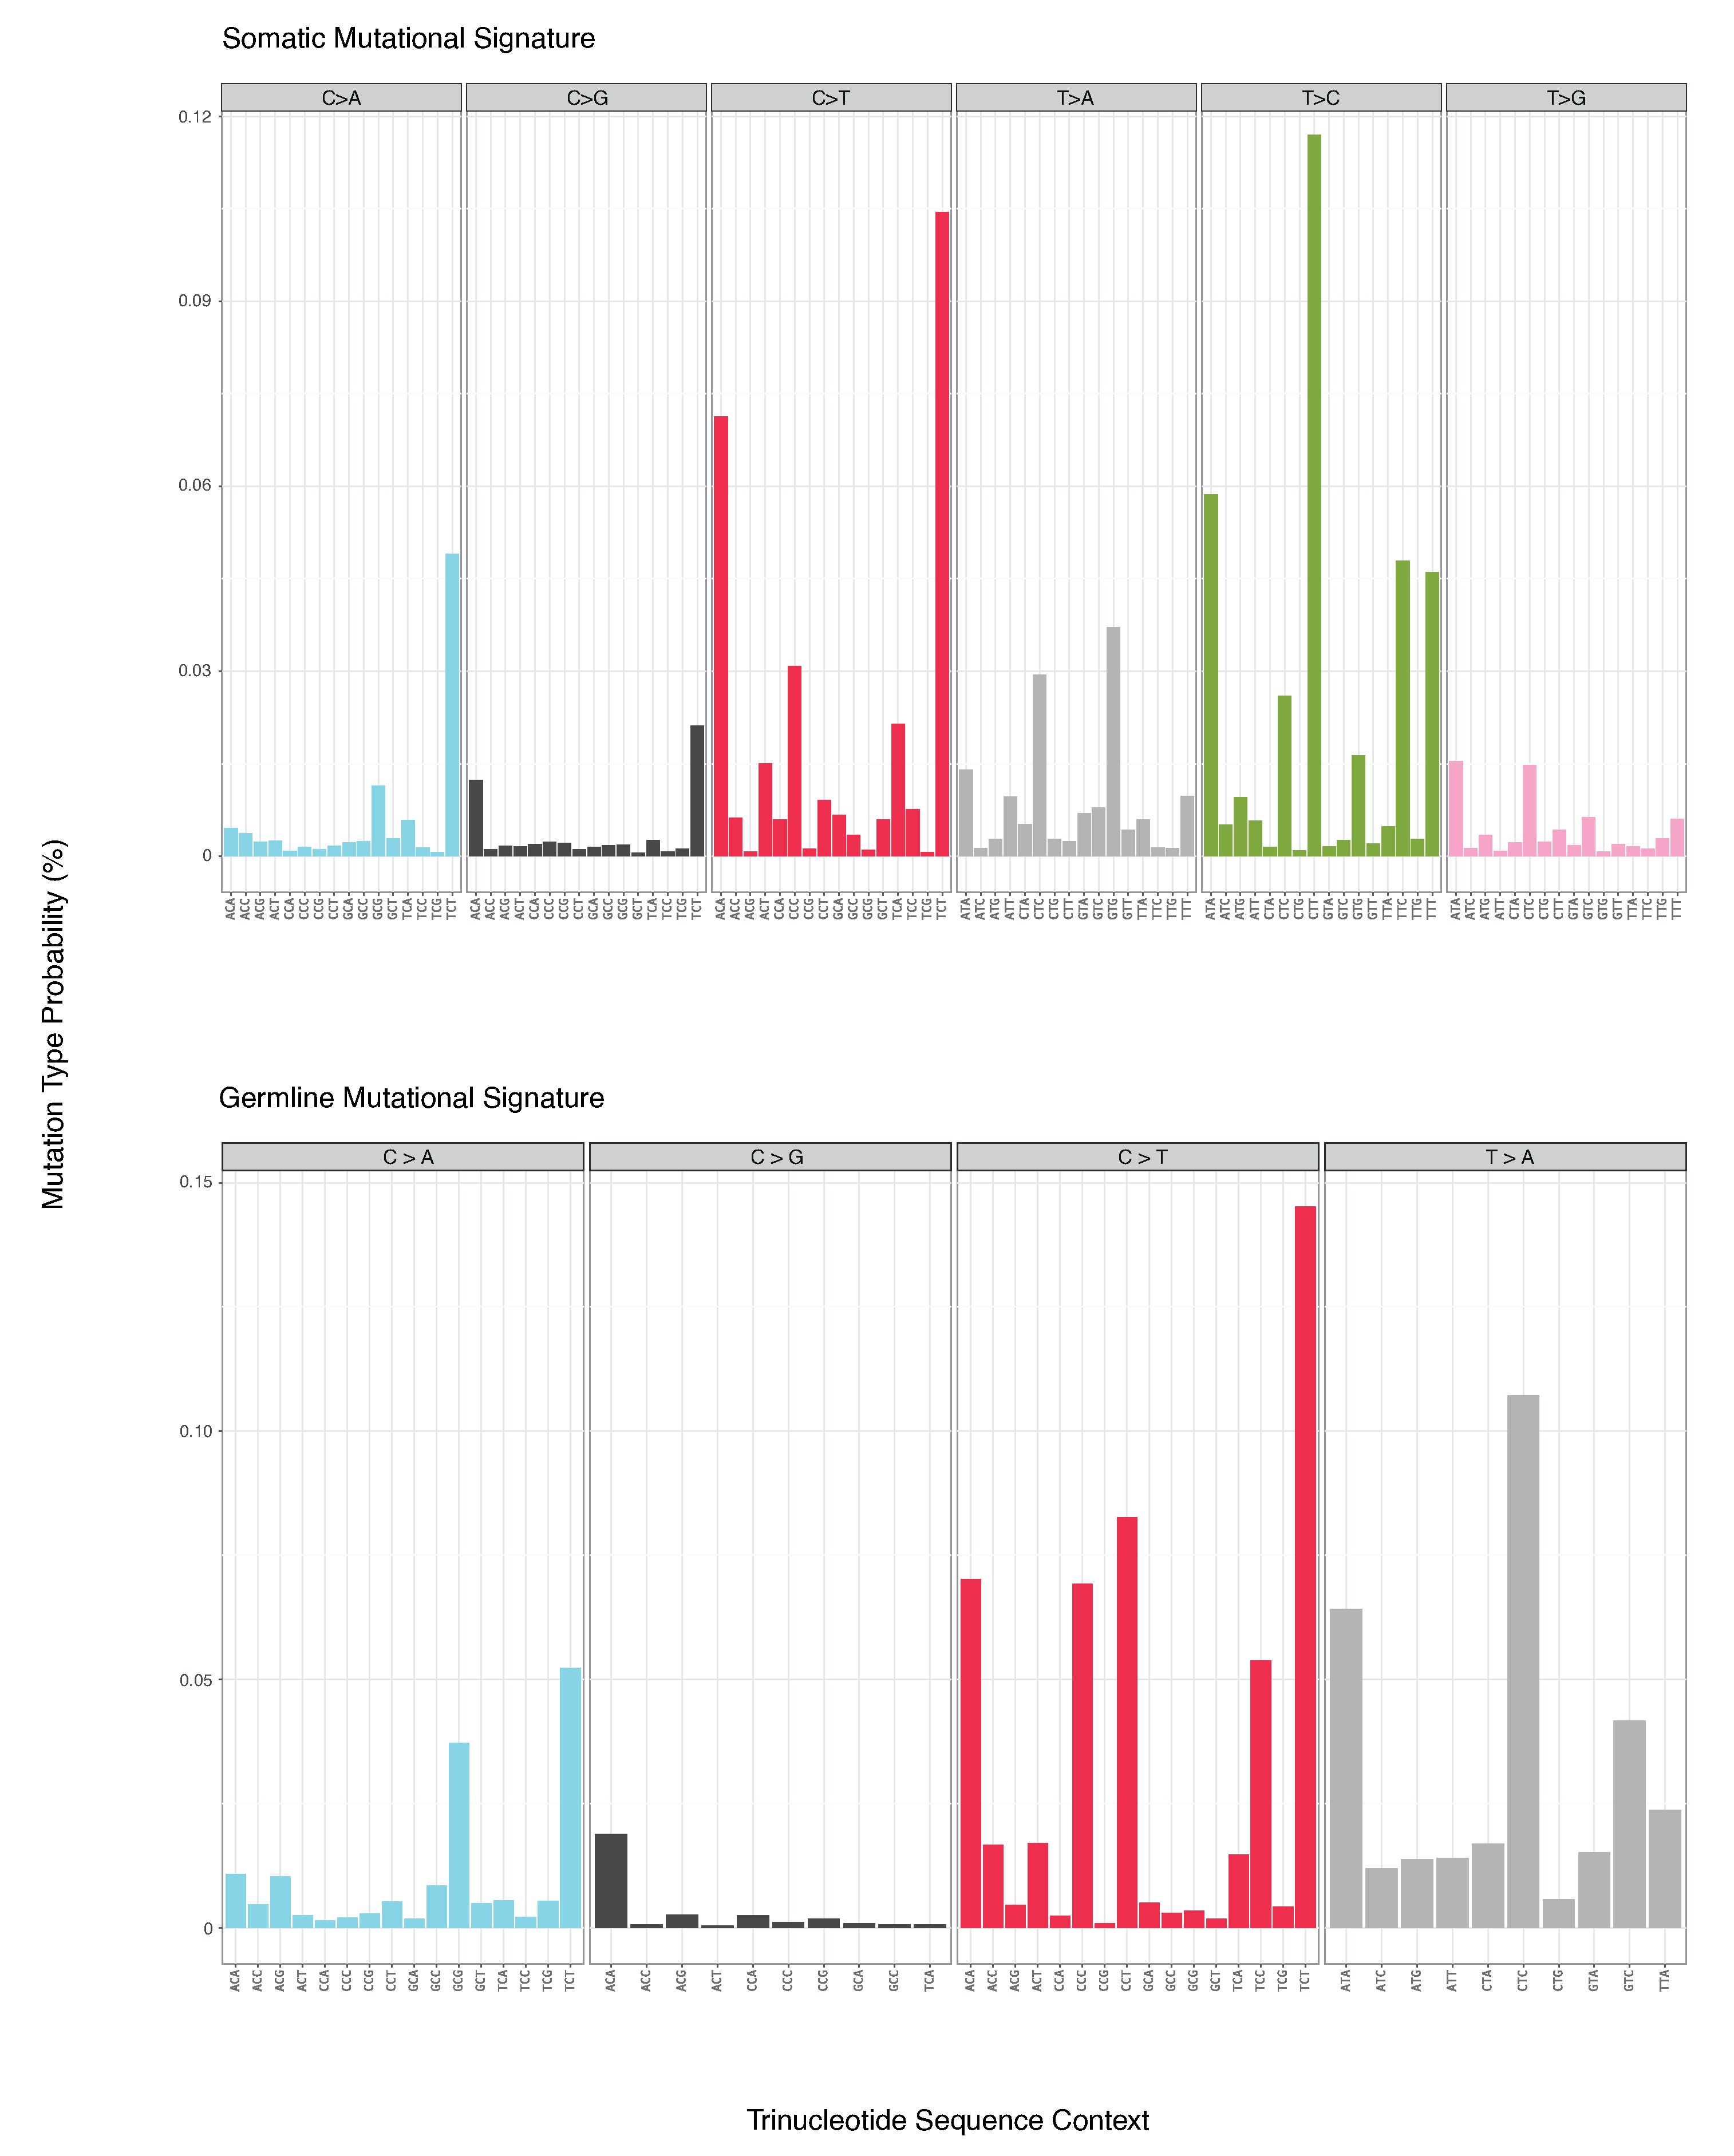
\includegraphics[width=\textwidth]{Vector/TOL6_signature.pdf}}
\end{centering}
\end{figure}

\begin{figure}[htbp!]
\caption{TOL signature 7 (TOL7)}
\label{figure:TOL7}
\begin{centering}
\makebox[\textwidth][c]{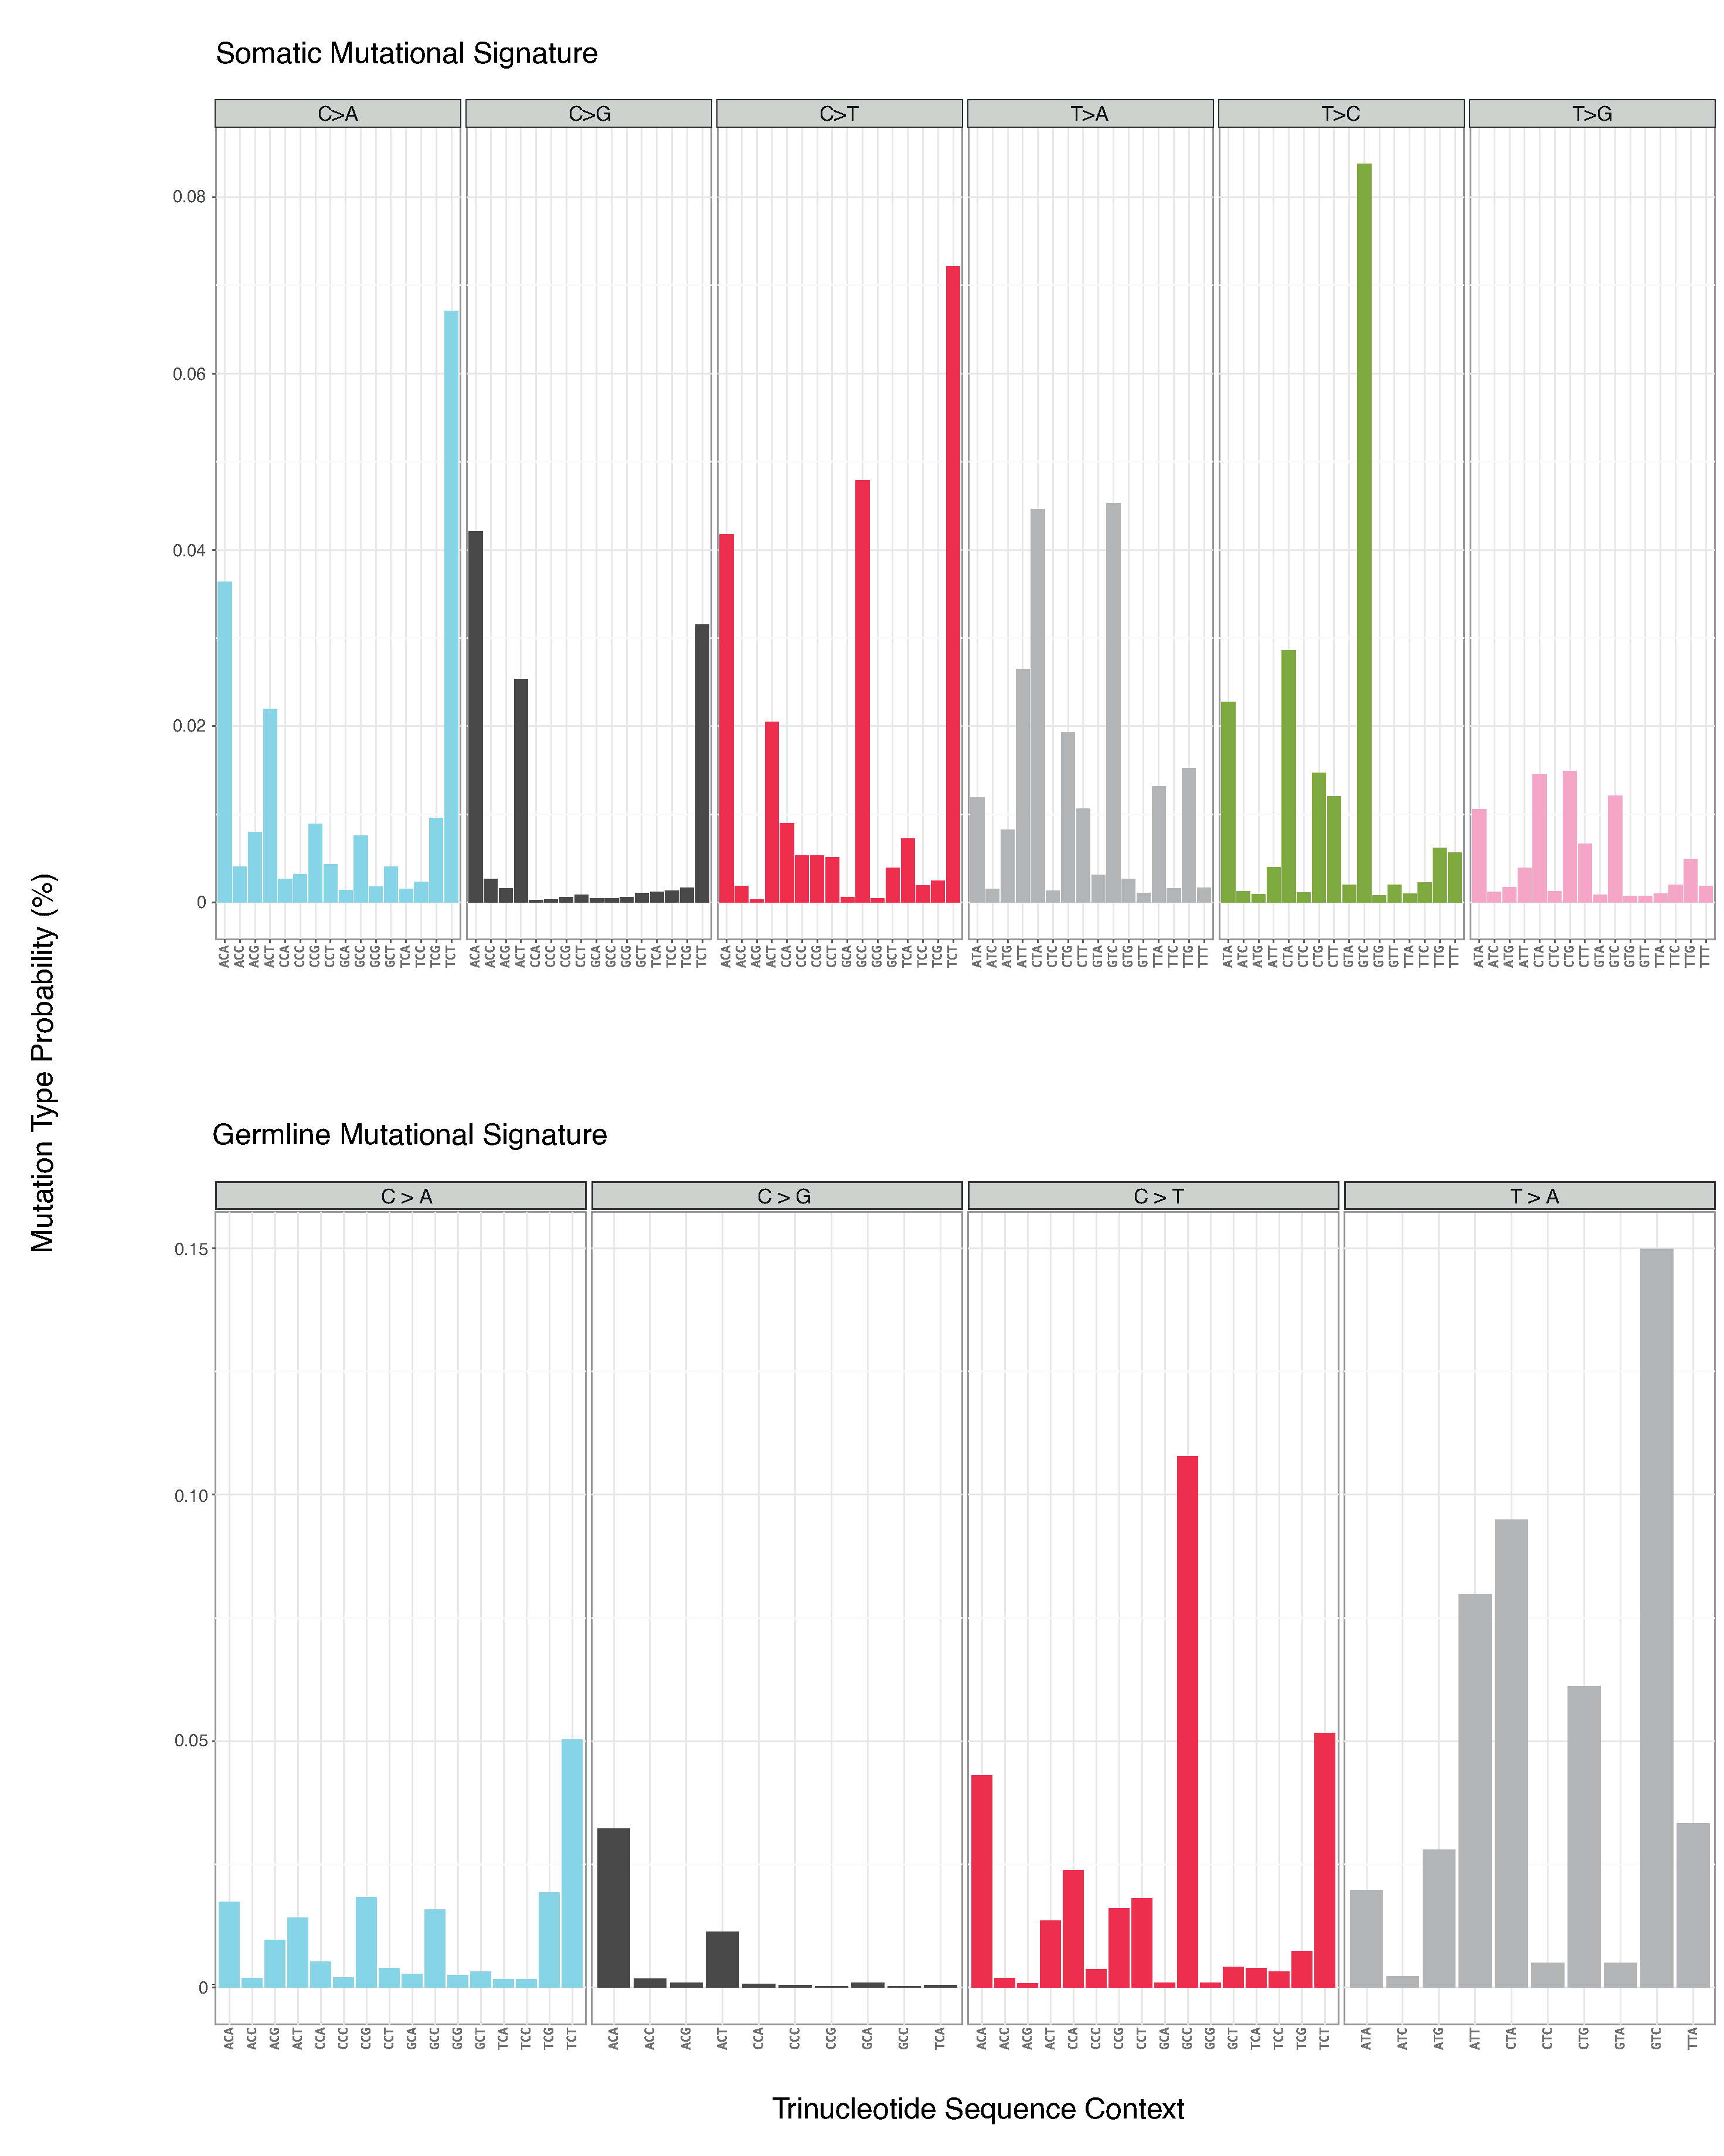
\includegraphics[width=\textwidth]{Vector/TOL7_signature.pdf}}
\end{centering}
\end{figure}

\begin{figure}[htbp!]
\caption{TOL signature 8 (TOL8)}
\label{figure:TOL8}
\begin{centering}
\makebox[\textwidth][c]{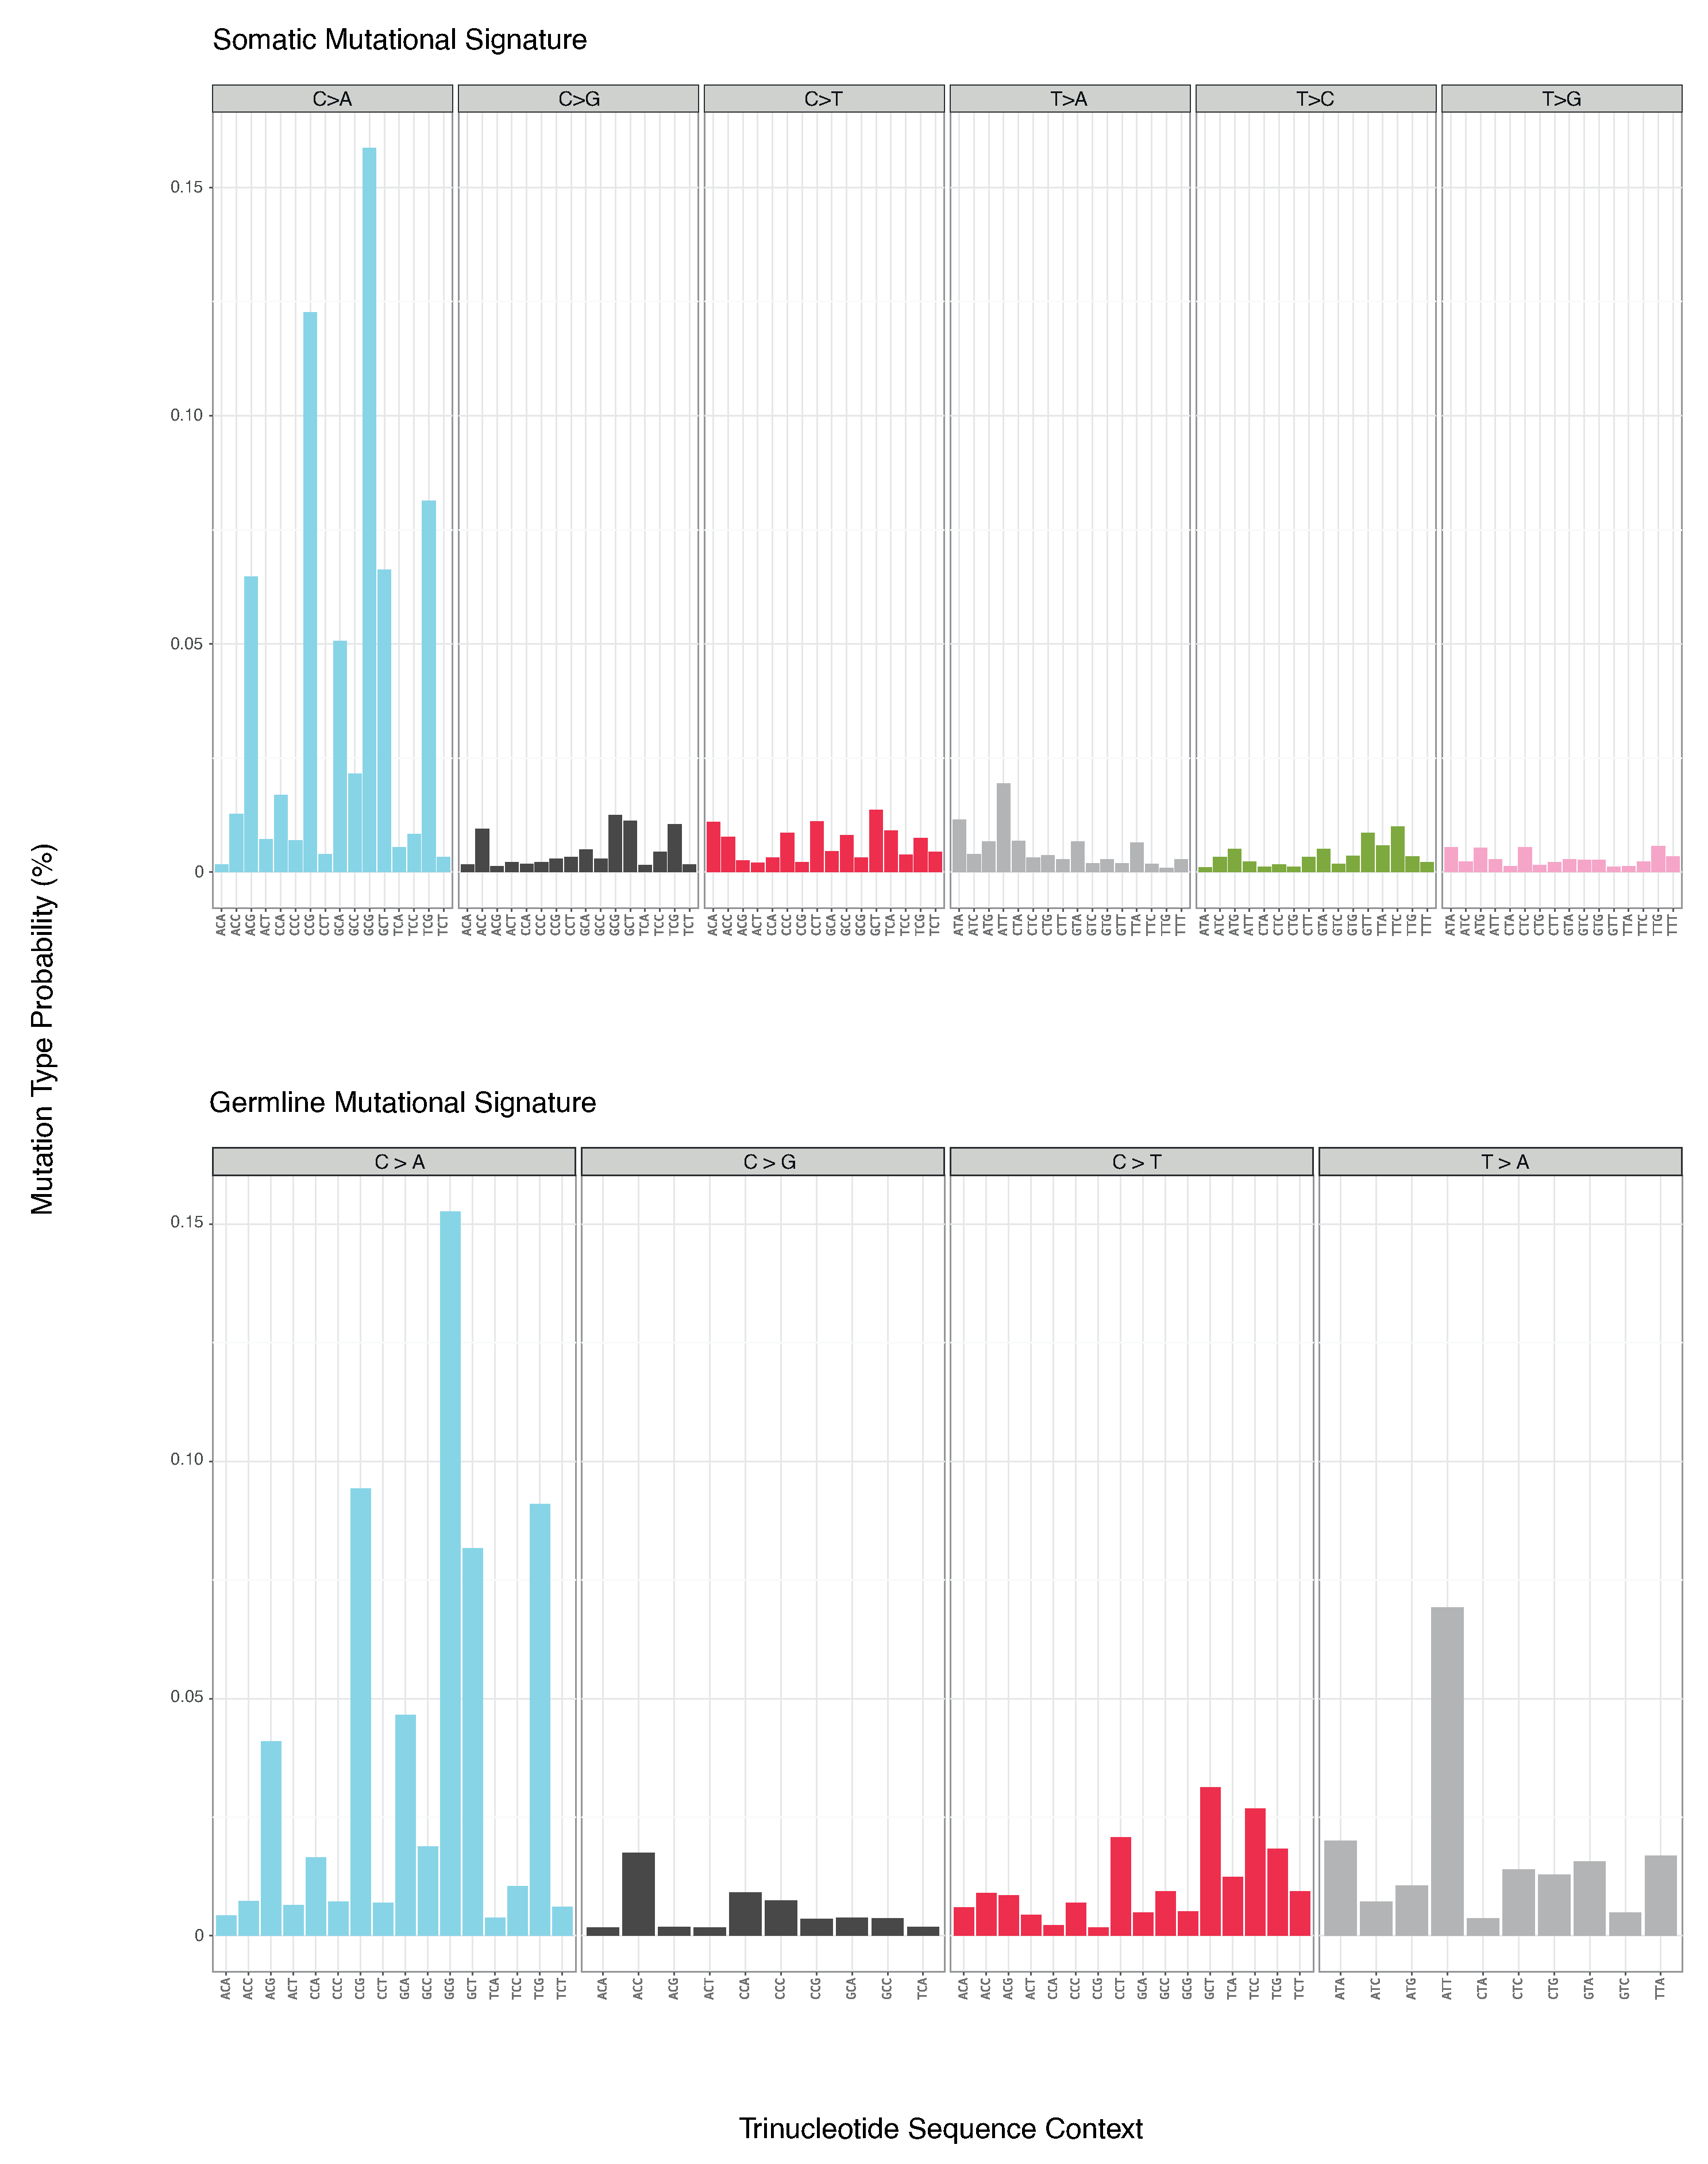
\includegraphics[width=\textwidth]{Vector/TOL8_signature.pdf}}
\end{centering}
\end{figure}

\begin{figure}[htbp!]
\caption{SBS96 and SBS192 somatic mutational spectra in \textit{S. pipiens}}
\label{figure:idSyrPipi1-SBS96-SBS192}
\begin{centering}
\makebox[\textwidth][c]{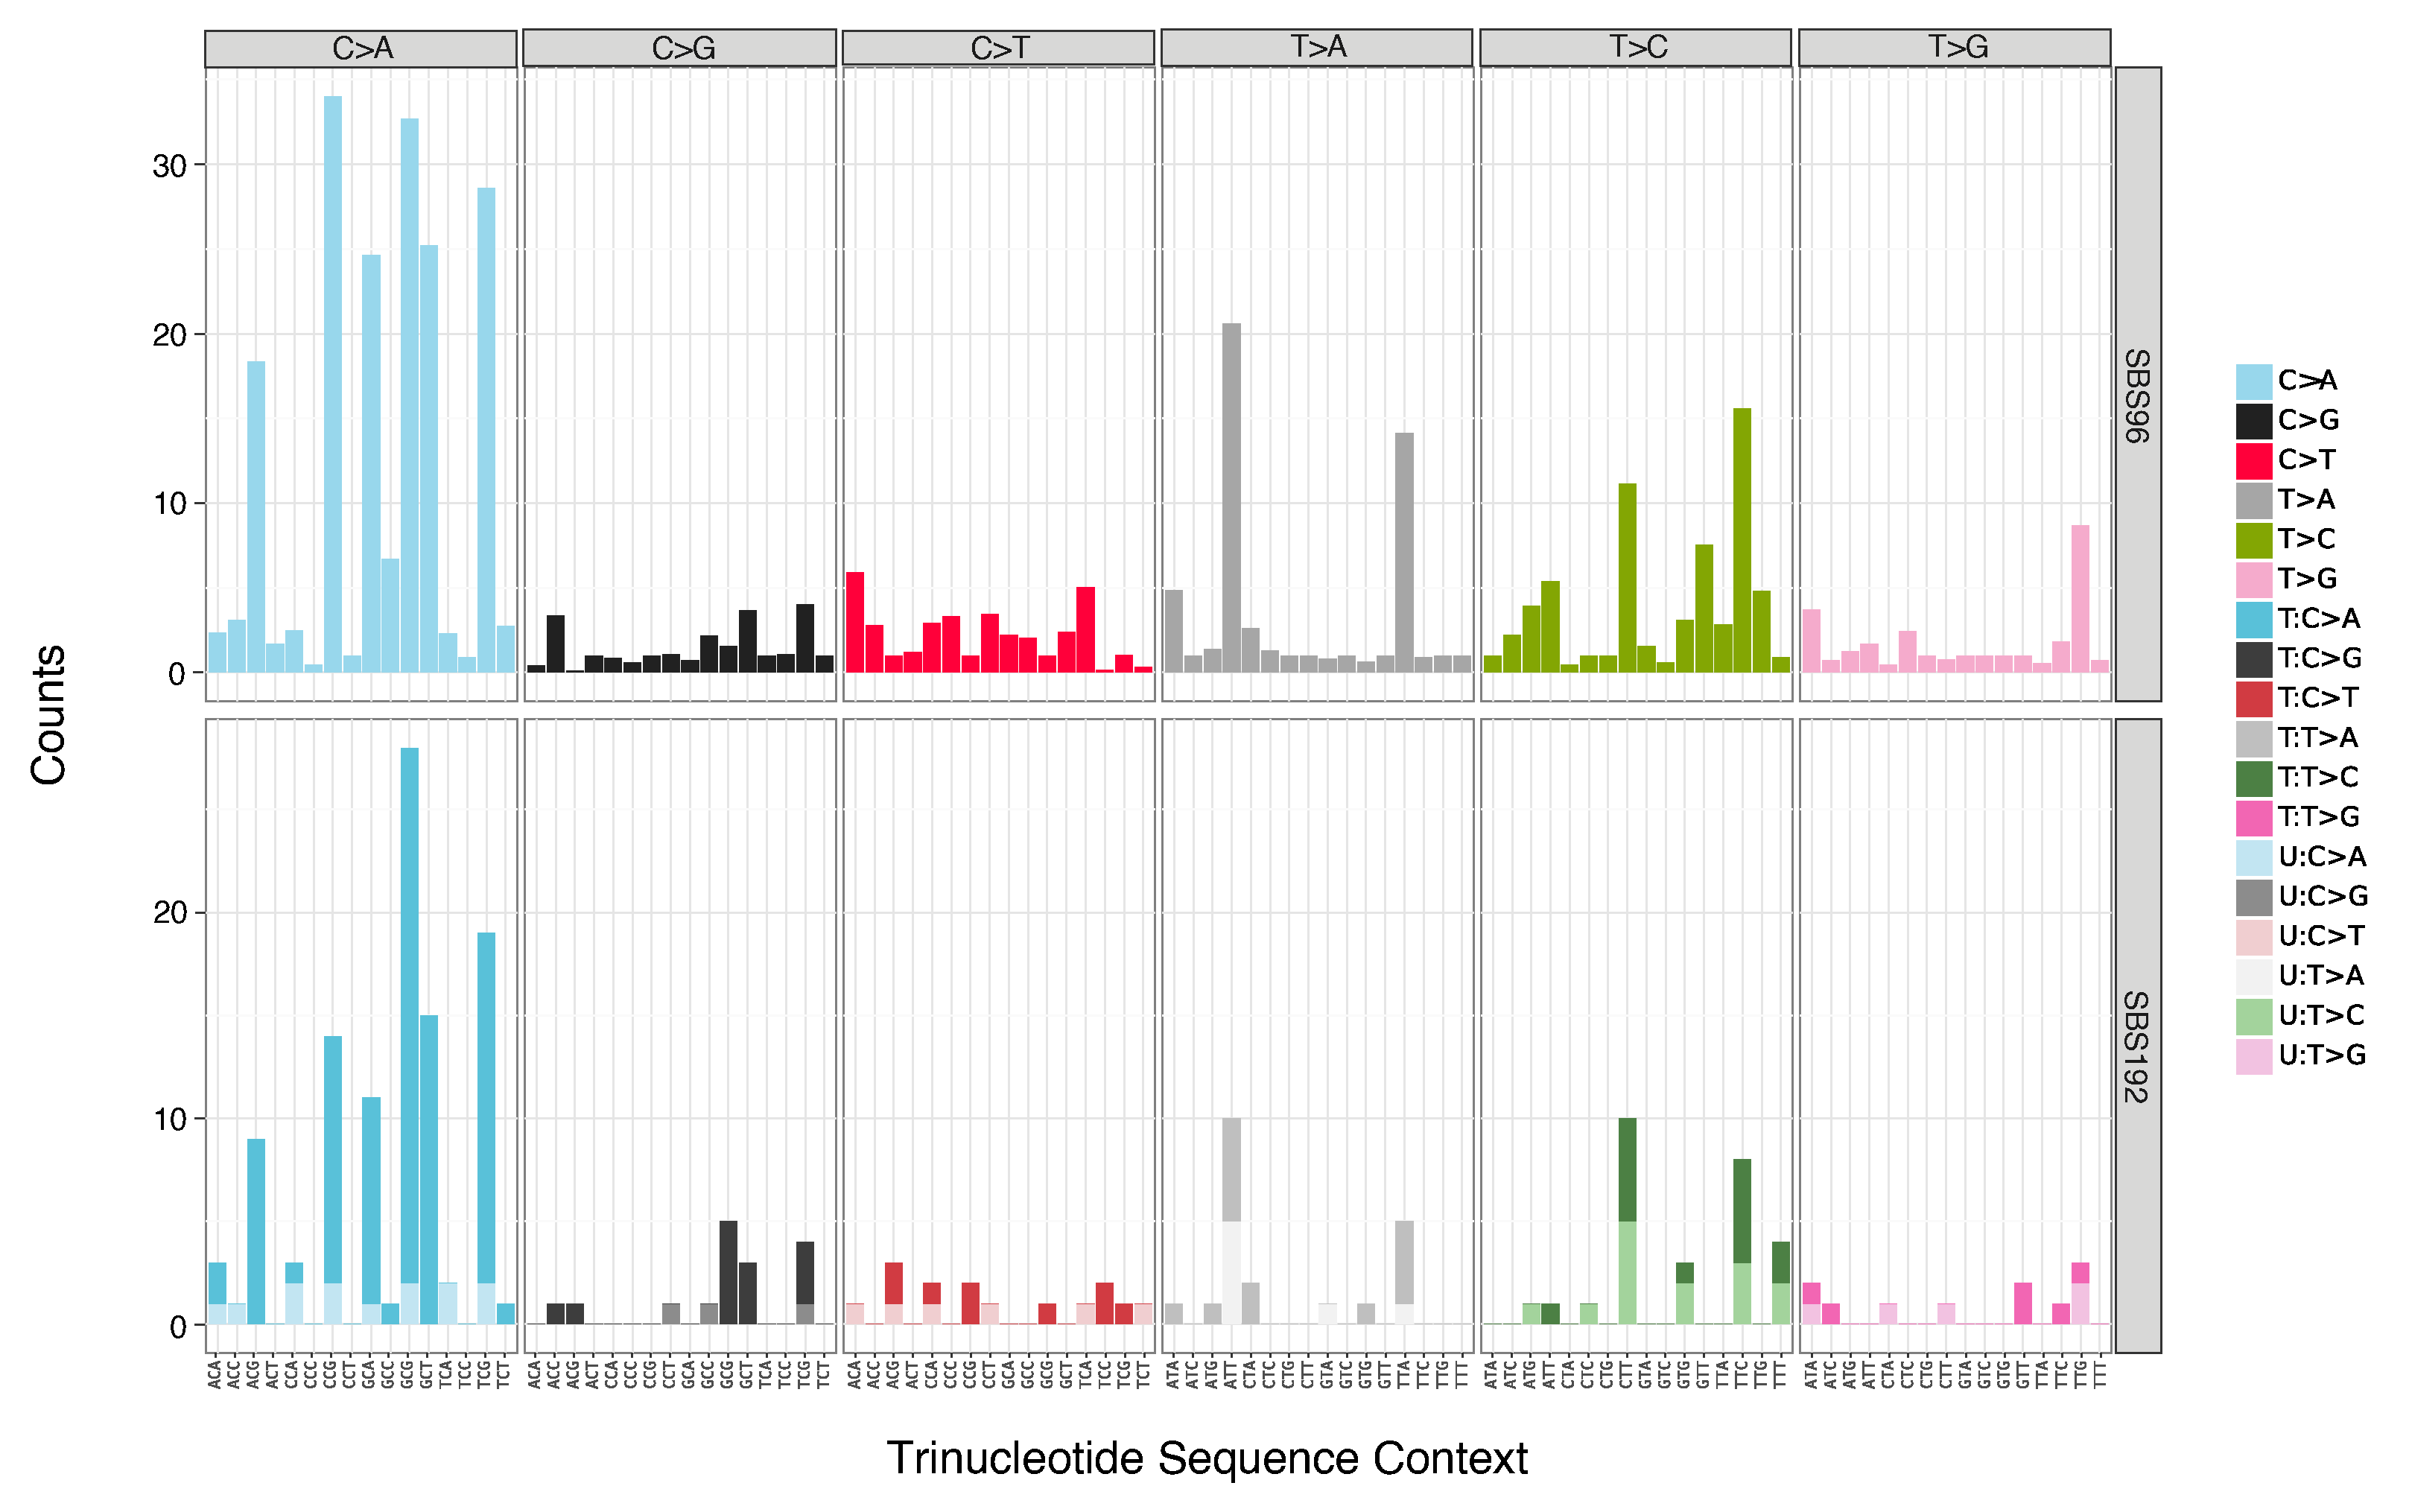
\includegraphics[width=\textwidth]{Vector/idSyrPipi1.somatic_sbs96_sbs192.pdf}}
\end{centering}
\floatfoot{T stands for transcribed and U stands for untranscribed. Inter-genic somatic mutations are excluded from SBS192 somatic mutational spectra.}
\end{figure}

\begin{figure}[htbp!]
\caption{TOL signature 9 (TOL9)}
\label{figure:TOL9}
\begin{centering}
\makebox[\textwidth][c]{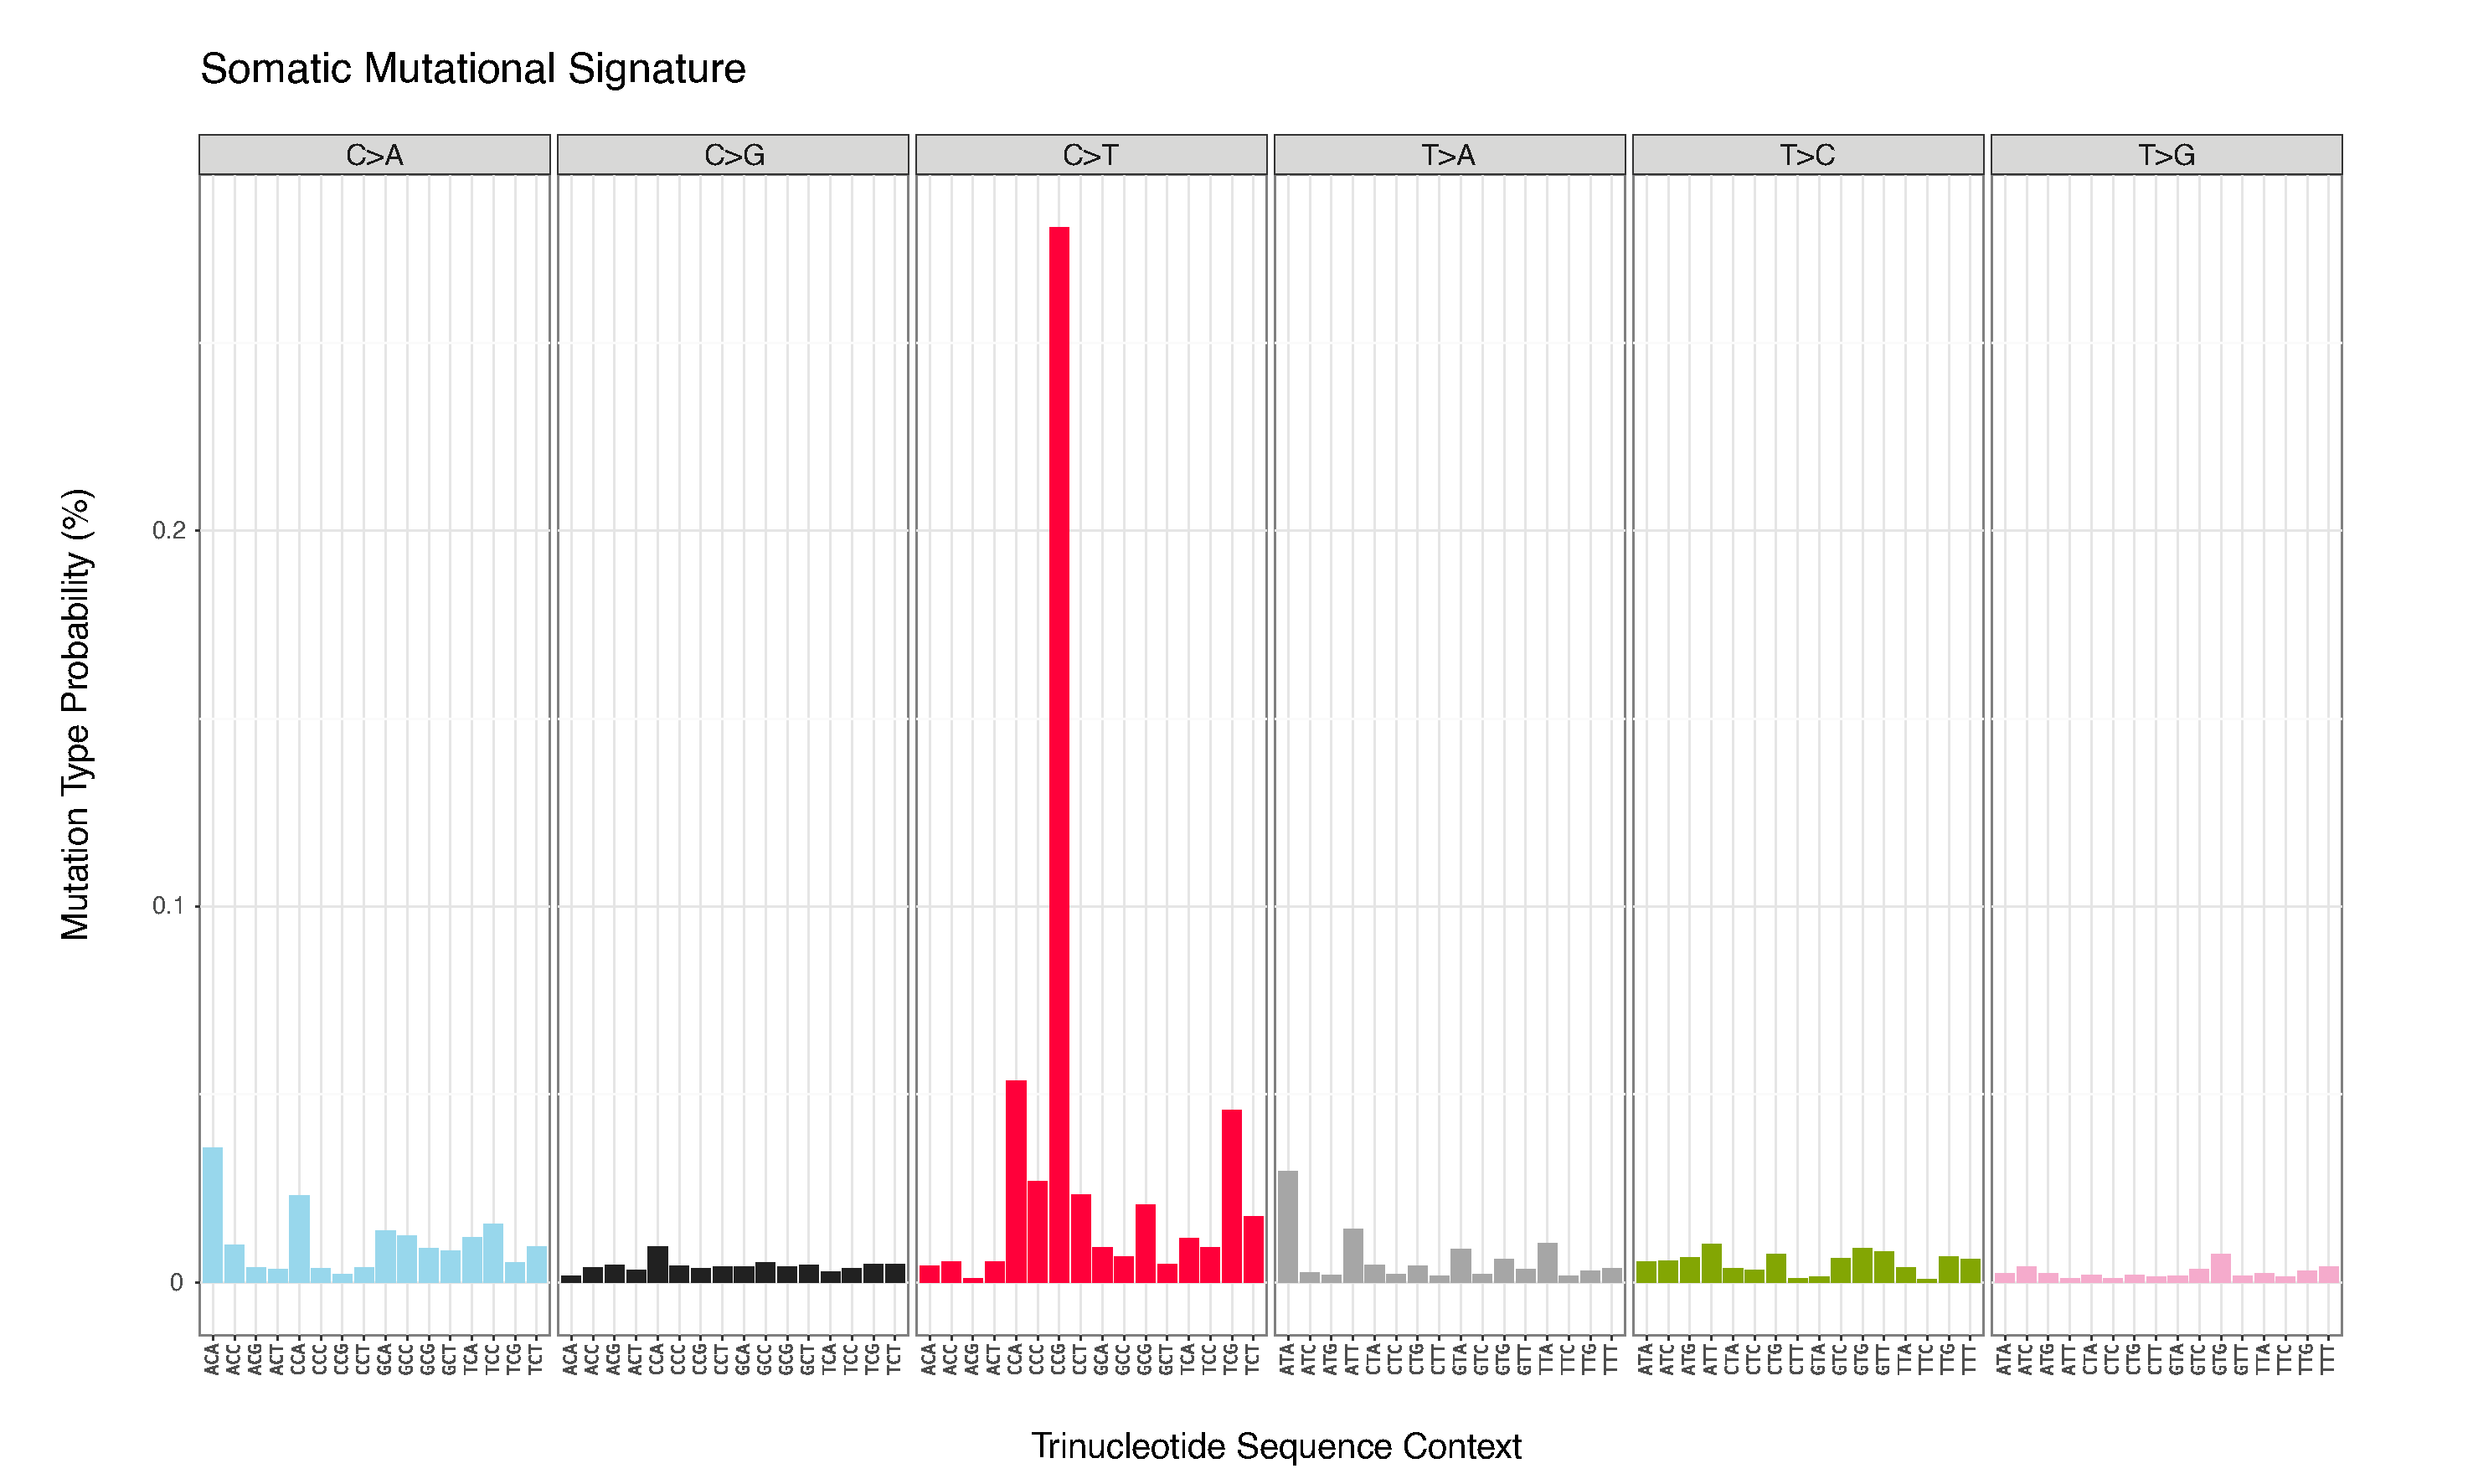
\includegraphics[width=\textwidth]{Vector/TOL9_signature.pdf}}
\end{centering}
\end{figure}

\begin{figure}[htbp!]
\caption{TOL signature 10 (TOL10)}
\label{figure:TOL10}
\begin{centering}
\makebox[\textwidth][c]{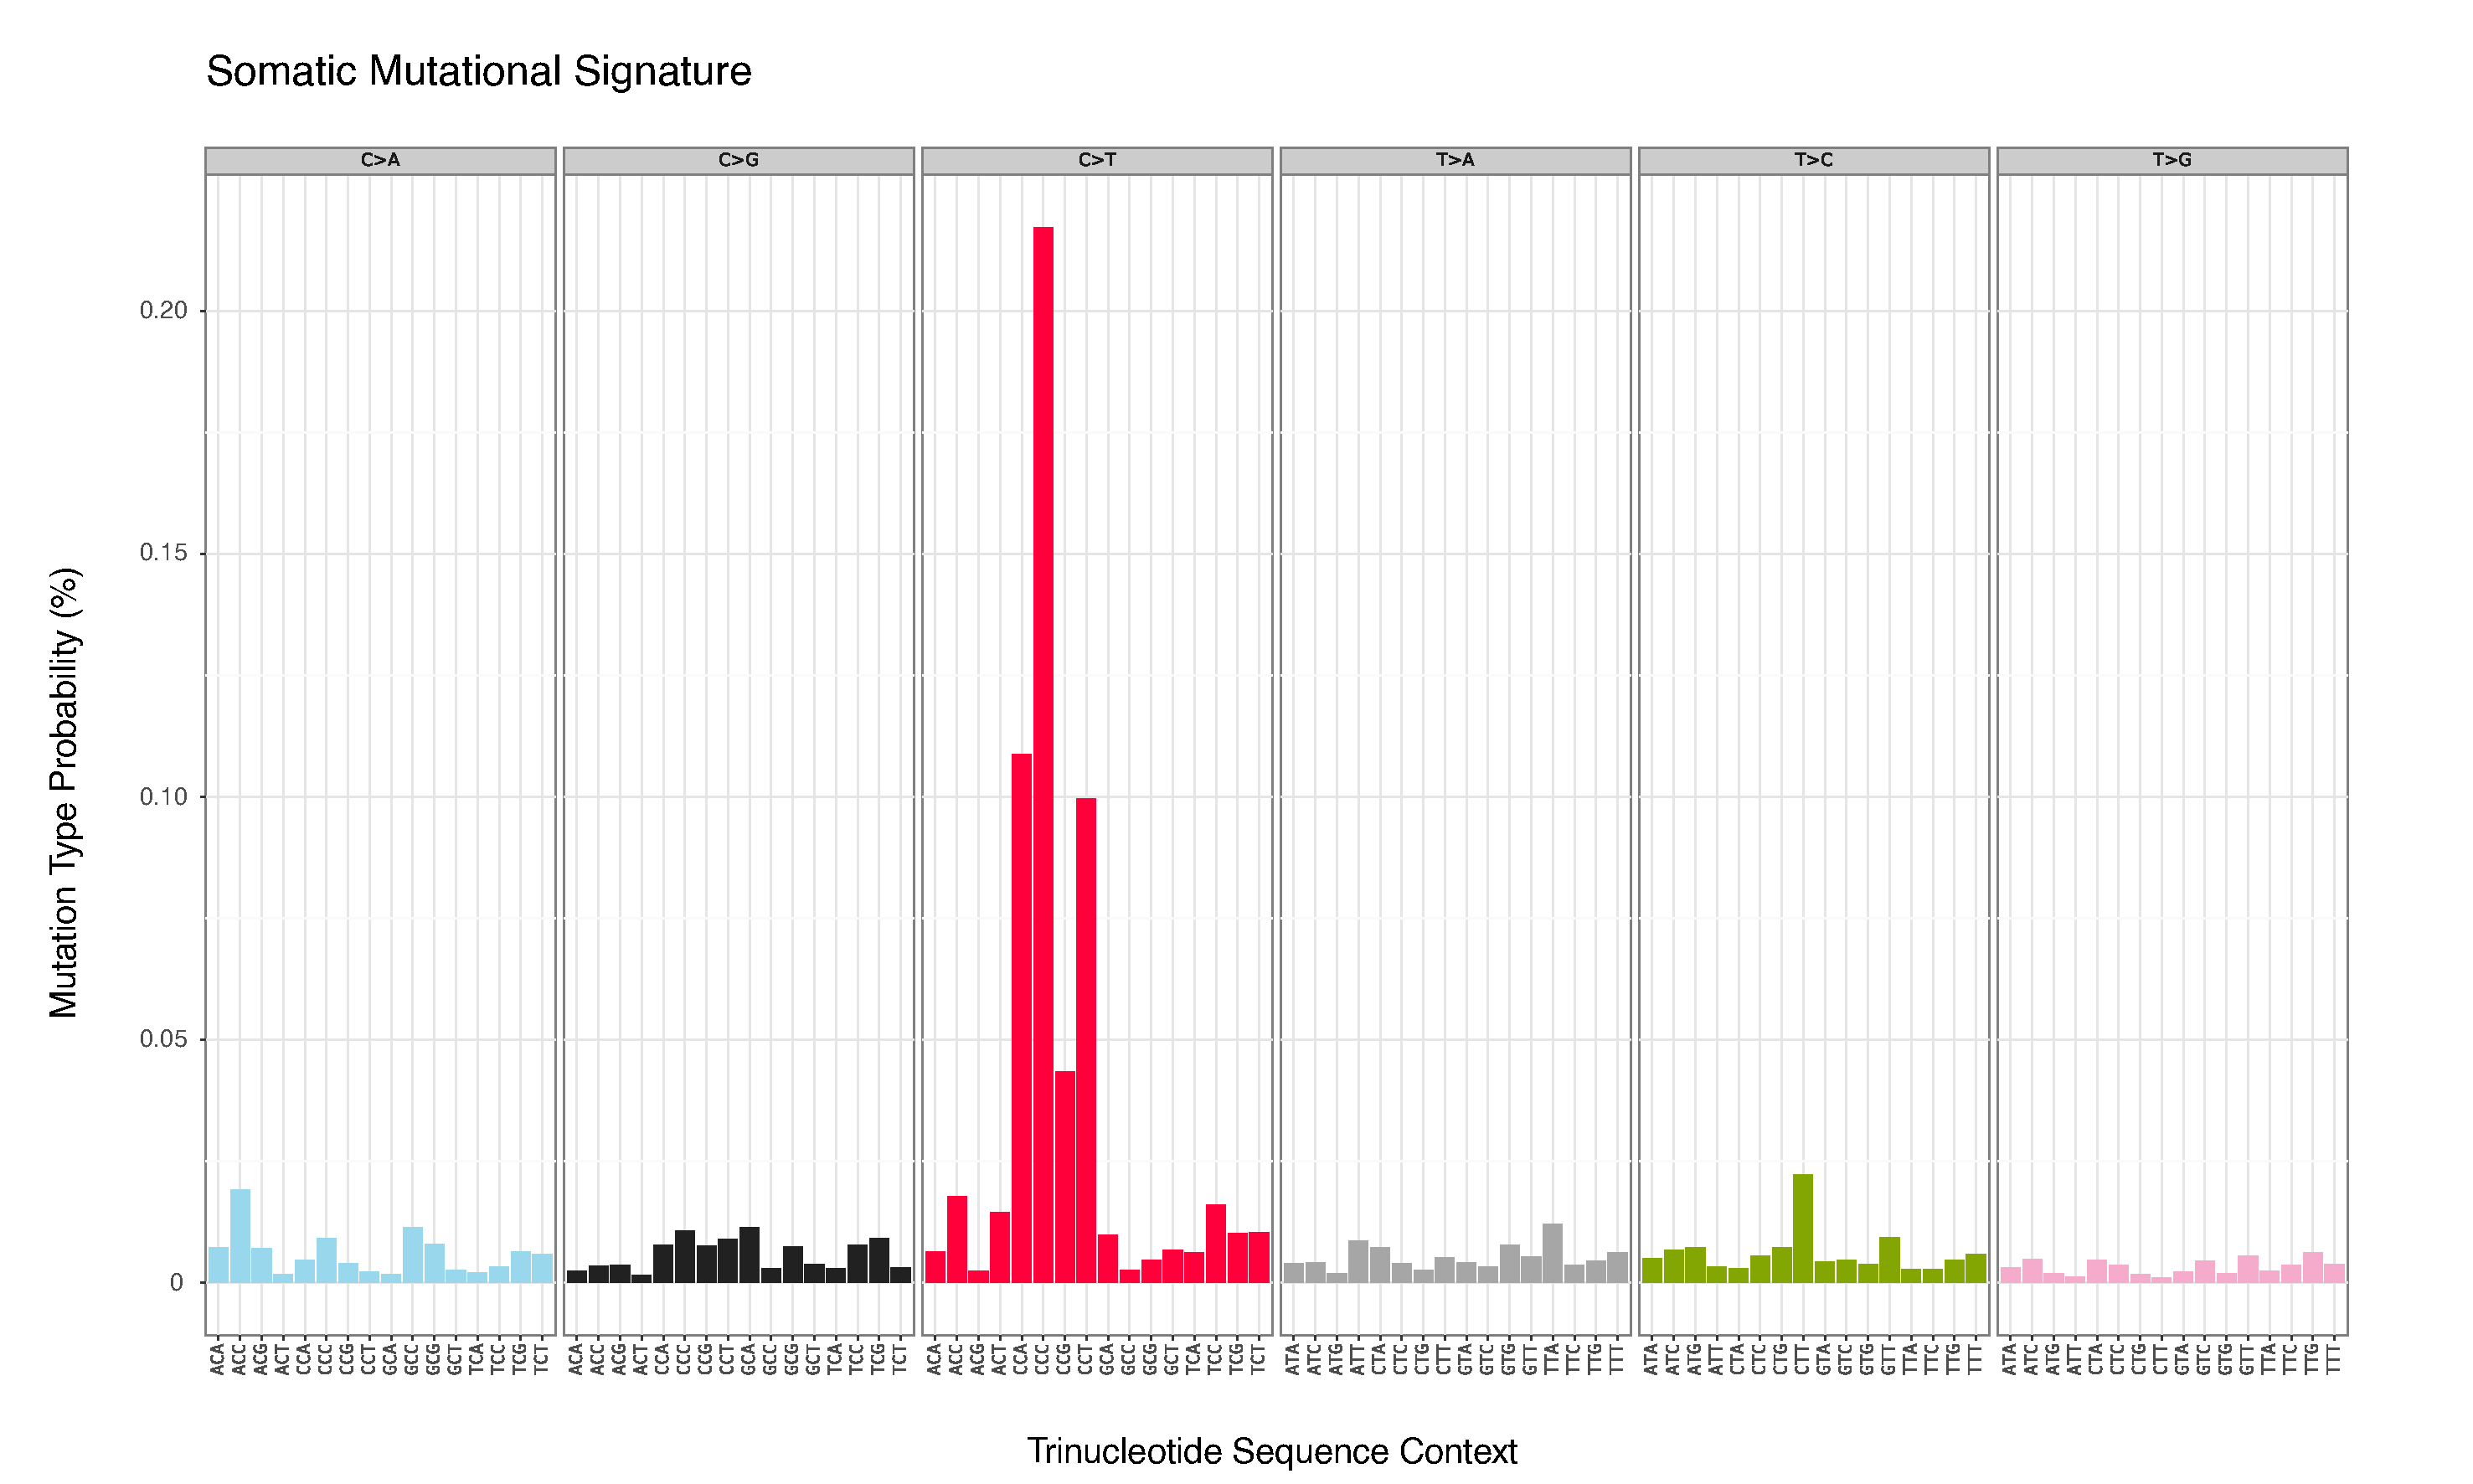
\includegraphics[width=\textwidth]{Vector/TOL10_signature.pdf}}
\end{centering}
\end{figure}

\begin{figure}[htbp!]
\caption{TOL signature 11 (TOL11)}
\label{figure:TOL11}
\begin{centering}
\makebox[\textwidth][c]{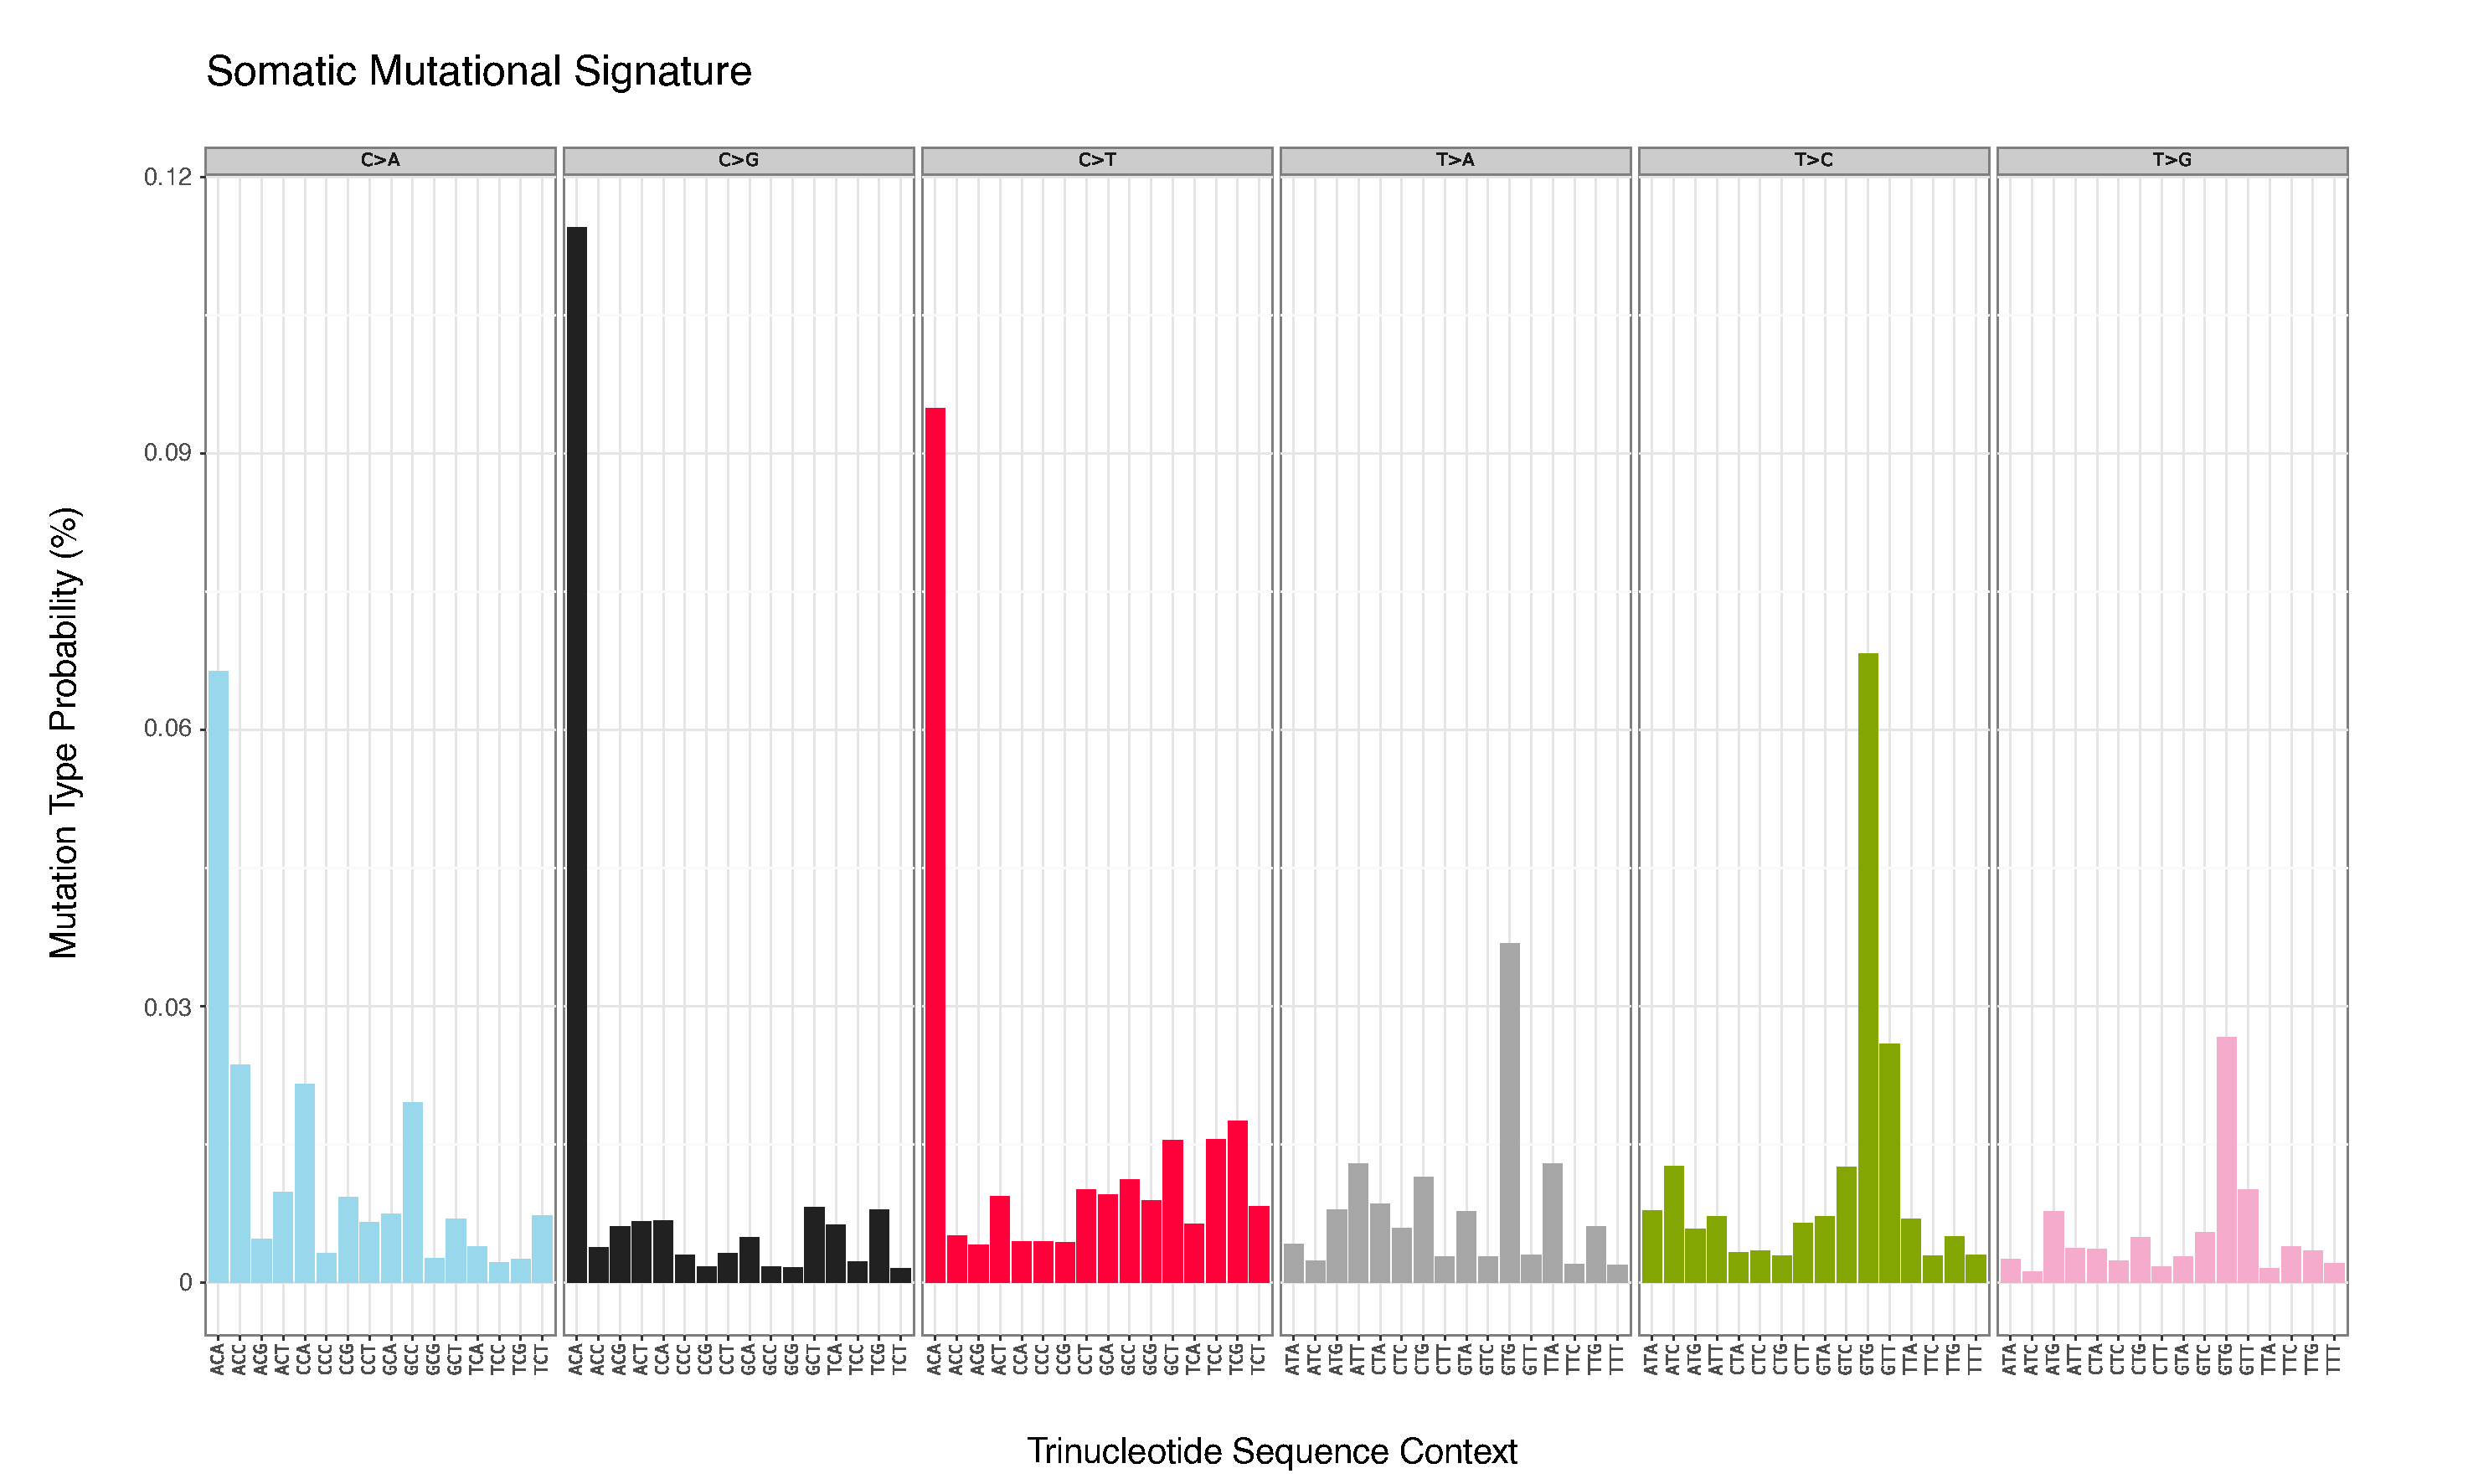
\includegraphics[width=\textwidth]{Vector/TOL11_signature.pdf}}
\end{centering}
\end{figure}

\begin{figure}[htbp!]
\caption{SBS96 and SBS192 somatic mutational spectra in \textit{P. albimanus}}
\label{figure:idPlaAlba1-SBS96-SBS192}
\begin{centering}
\makebox[\textwidth][c]{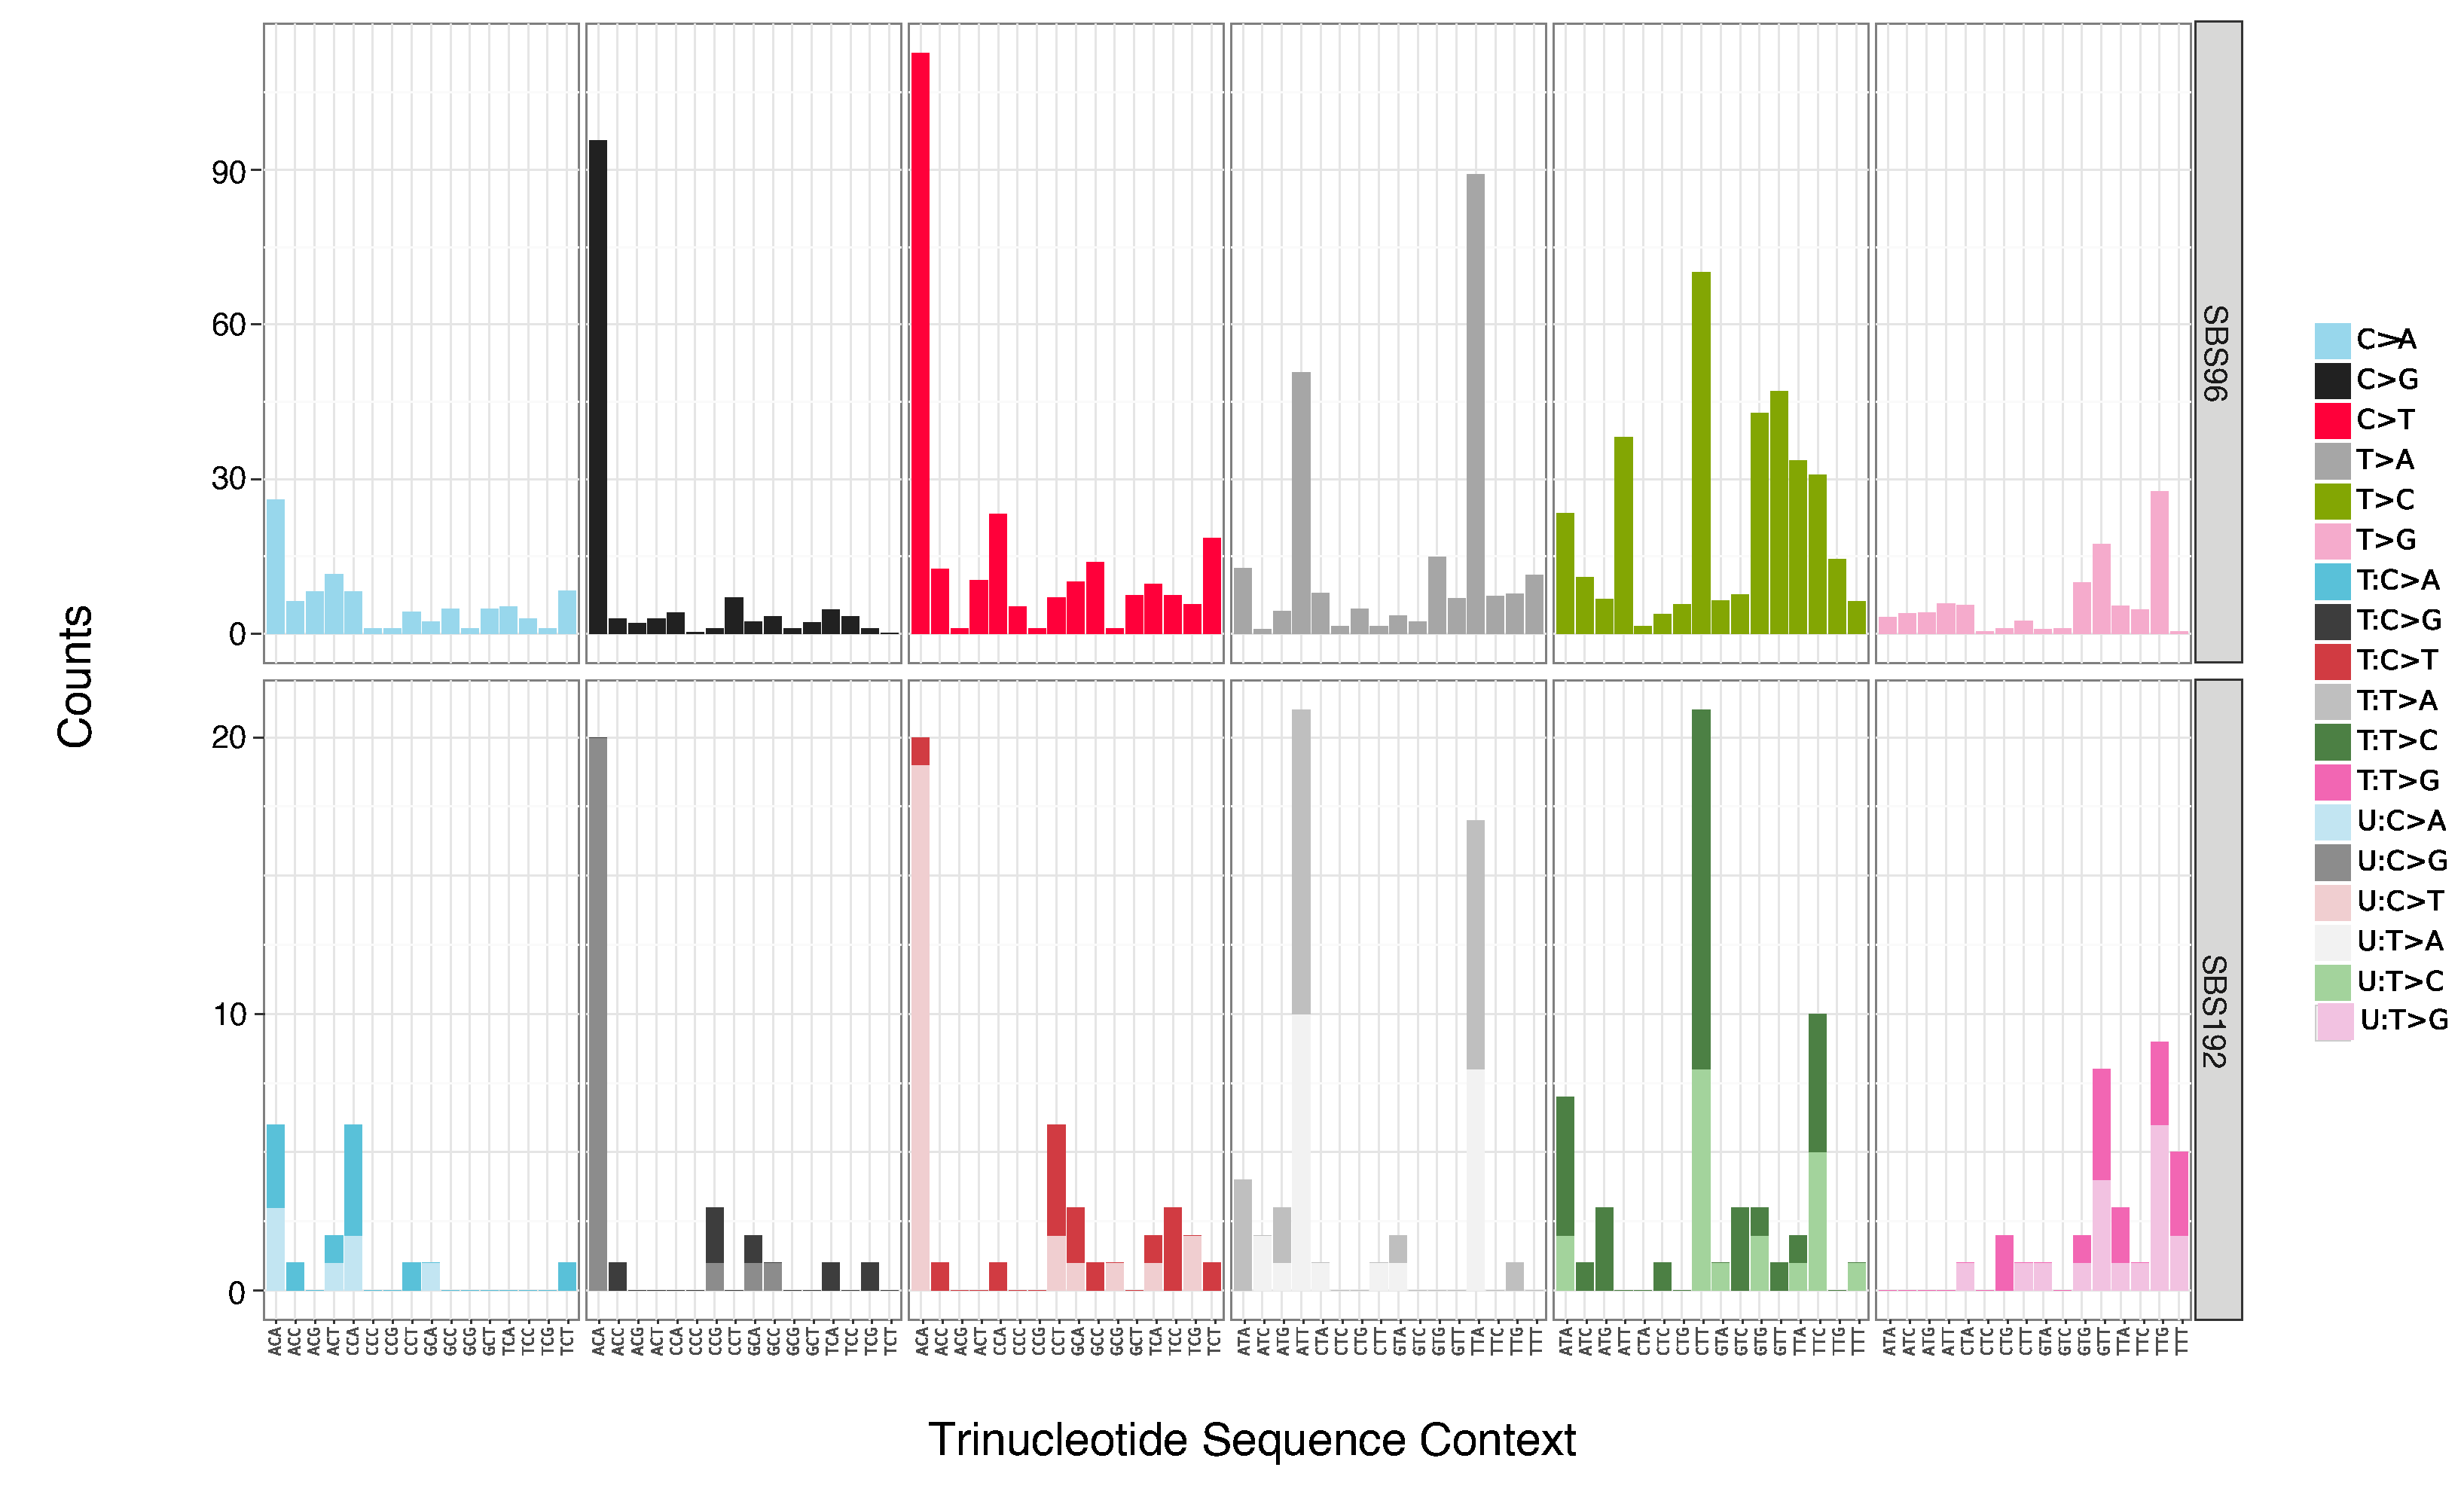
\includegraphics[width=0.9\textwidth]{Vector/idPlaAlba1.somatic_sbs96_sbs192.pdf}}
\end{centering}
\floatfoot{T stands for transcribed and U stands for untranscribed. Inter-genic somatic mutations are excluded from SBS192 somatic mutational spectra.}
\end{figure}

\pagebreak

\section{Conclusion}

In chapter 2, I described the design of himut and demonstrated the use of himut for single-molecule somatic mutation detection from normal bulk human tissue and lymphoma and colorectal cancer cell lines. In this chapter, I show that himut can be used for somatic mutation detection in non-human samples and additionally, that mutational signatures, which represent the probability of a somatic mutational processes introducing a new somatic mutation within a specific sequence context, can be successfully extracted from somatic mutations called in non-human samples. 

Based on the genetic and epigenetic information regarding the sample, as well as the phylogenetic relationship between the samples, I identified 2 error signatures and 11 mutational signatures. Furthermore, I have also determined when this somatic mutational process emerged based on when the most recent common ancestor that possessed these somatic mutational processes appeared in the phylogenetic tree. 


